%%%%%%%%%%%%%%%%%%%%%%%%%%%%%%%%%%%%%%%%%
% Masters/Doctoral Thesis 
% LaTeX Template
% Version 1.43 (17/5/14)
%
% This template has been downloaded from:\documentclass[options]{class}
% http://www.LaTeXTemplates.com
%
% Current author:
% Some items were added and modified by for use in 
% undergraduate Final Year Project (FYP) at
% Multimedia University, Cyberjaya, Malaysia.
% Wan Ruslan Yusoff 
% wruslan@mmu.edu.my
%
% Original authors:
% Steven Gunn 
% http://users.ecs.soton.ac.uk/srg/softwaretools/document/templates/
% and
% Sunil Patel
% http://www.sunilpatel.co.uk/thesis-template/
%
% License:
% CC BY-NC-SA 3.0 (http://creativecommons.org/licenses/by-nc-sa/3.0/)
%
% Note:
% Make sure to edit document variables in the Thesis.cls file
%
%%%%%%%%%%%%%%%%%%%%%%%%%%%%%%%%%%%%%%%%%
%----------------------------------------------------------------------------------------
%	PACKAGES AND OTHER DOCUMENT CONFIGURATIONS
%----------------------------------------------------------------------------------------

\documentclass[12pt, oneside]{Thesis} 
% The default font size and one-sided printing (no margin offsets)

\graphicspath{{Pictures/}} 
% Specifies the directory where pictures are stored
\usepackage{float} 
% To make picture stay at placement
\usepackage{pdfpages}
\usepackage{setspace} 

\usepackage{algorithm}
\usepackage{algpseudocode}

\usepackage{lscape}

% Double spacing
%\doublespacing % Use on each page

\usepackage[square, numbers, comma, sort&compress]{natbib} 
% Use the natbib reference package - read up on this to edit the reference style; if you want text (e.g. Smith et al., 2012) for the in-text references (instead of numbers), remove 'numbers' 
\usepackage{hyperref}
\hypersetup{urlcolor=black, colorlinks=true} 
% Colors hyperlinks in blue - change to black if annoying


\title{\ttitle} 
% Defines the thesis title - don't touch this

% ================================================
% % ADDED BY WRY
\usepackage{caption}
\usepackage{appendix}
\usepackage{tikz}
\usepackage[europeanresistors,americaninductors]{circuitikz}
\usetikzlibrary{chains}

% ================================================
% % ADDED BY CHARLES
\usepackage{tabulary}
\usepackage{graphicx}
\usepackage{pdfpages}
\usepackage{enumitem}

% ==================================================
\begin{document}
% ==================================================


\frontmatter 
% Use roman page numbering style (i, ii, iii, iv...) for the pre-content pages

\setstretch{1.3} 
% Line spacing of 1.3

% Define the page headers using the FancyHdr package and set up for one-sided printing
\fancyhead{}

% Clears all page headers and footers
\rhead{\thepage}

% Sets the right side header to show the page number
\lhead{}
% Clears the left side page header

\pagestyle{fancy} 
% Finally, use the "fancy" page style to implement the FancyHdr headers

\newcommand{\HRule}{\rule{\linewidth}{0.5mm}} 
% New command to make the lines in the title page

% PDF meta-data
\hypersetup{pdftitle={\ttitle}}
\hypersetup{pdfsubject=\subjectname}
\hypersetup{pdfauthor=\authornames}
\hypersetup{pdfkeywords=\keywordnames}

%----------------------------------------------------------------------------------------
%	TITLE PAGE
%----------------------------------------------------------------------------------------

\begin{titlepage}
\begin{center}

{\LARGE \ttitle}\\[0.4cm] 
\vfill
\Large{CHAI YING HUA} 

\vfill
\normalsize{SESSION 2017/2018}
\vfill
\normalsize\FACNAME\\
\normalsize \UNIVNAME\\
{\normalsize SEPTEMBER 2017}\\ 
\vfill
\end{center}

\end{titlepage}
\thispagestyle{empty}
\begin{center}

	{\LARGE \ttitle}\\[0.4cm] % Thesis title
	\vfill
	\footnotesize{BY}
	\vfill
	\Large{CHAI YING HUA} % Author name - remove the \href bracket to remove the link
	\vfill
	\footnotesize{SESSION 2017/2018}
	\vfill
	\footnotesize{THIS PROJECT REPORT IS PREPARED FOR}
	\vfil
	\normalsize\FACNAME\\
	\normalsize \UNIVNAME\\
	\normalsize{IN PARTIAL FULFILLMENT}\\
	\normalsize{FOR}\\
	\vfil
	\normalsize{BACHELOR OF COMPUTER SCIENCE (HONS)}\\
	\normalsize{WITH SPECIALIZATION IN}\\
	\normalsize{SOFTWARE ENGINEERING}\\
	\vfil
	\normalsize\FACNAME\\
	\vfil
	\Large \UNIVNAME\\
	\vfil
	{\normalsize FEBRUARY 2018}\\ % Date
	%\includegraphics{Logo} % University/department logo - uncomment to place it
	\vfill
\end{center}

\newpage
\thispagestyle{empty}

The copyright of this thesis belongs to the author under the terms of the Copyright Act 1987 as qualified by Regulation 4(1) of the Multimedia University Intellectual Property Regulations. Due acknowledgment shall always be made of the use of any material contained in, or derived from, this thesis. 

\vfil
\textit{© Chai Ying Hua, 2018}\\
All rights reserved


%----------------------------------------------------------------------------------------
%	DECLARATION PAGE
%	Your institution may give you a different text to place here
%----------------------------------------------------------------------------------------
\newpage
\Declaration{

\addtocontents{toc}{\vspace{1em}} 
% Add a gap in the Contents, for aesthetics

I hereby declare that the work in this thesis have been done by myself and no portion of the work contained in this thesis has been submitted in support of any application for any other degree or qualification of this or any other university or institute of learning.

\vfill

\rule[1em]{25em}{0.5pt} % This prints a line for the signature
\\Name: \textit{Chai Ying Hua}
\\Student ID: 1141328508
\\Faculty of Computing \& Informatics
\\Multimedia University
\\Date: 7$^{th}$ February 2018

}

\clearpage % Start a new page

%----------------------------------------------------------------------------------------
%	ACKNOWLEDGEMENTS
%----------------------------------------------------------------------------------------

\setstretch{1.3} % Reset the line-spacing to 1.3 for body text (if it has changed)

\acknowledgements{\addtocontents{toc}{\vspace{1em}} % Add a gap in the Contents, for aesthetics
\begin{flushleft}

The success and outcome of this project require tons of guidance and assistance from many people, and I am blessed and appreciate to have got this all along the completion of my project. My project would not be complete smoothly without their helping hands.

First and foremost, I would like to express sincere gratitude to my project supervisor, Mr Wan Ruslan Yusoff of Faculty of Computing Informatics at Multimedia University Cyberjaya for your unfailing support and assistance on my project. The door to Ruslan office and his mailbox was always open whenever I faced any impediment and trouble about my project or writing. He consistently and patiently steered me in the right direction whenever he thought I needed it. Also, he is eager to share his expertise and industrial experience in computing fields and provide encouragement and motivation on my project.

I owe gratitude to my parents for providing chances and opportunity for me to study in Multimedia University. They are caring, and concern about my academic and regularly provide support and attention on cultivating me to get myself prepare for an upcoming challenge.

Last but not least, I place on record, my sense of gratitude to my friend and classmate, who directly and indirectly unceasing encouragement and provide guidance till the completion of my project.
  

\end{flushleft}
}
\clearpage % Start a new page

%----------------------------------------------------------------------------------------
%	ABBREVIATIONS AND ACRONYMS 
%----------------------------------------------------------------------------------------
%% ADDED BY WRY

\pagestyle{fancy} % The page style headers have been "empty" all this time, now use the "fancy" headers as defined before to bring them back
%
\pagebreak
\addtotoc{Abbreviations and Acronyms} 
\lhead{\normalfont\huge{Abbreviations and Acronyms}}
%
%
%% TABLE HEADER
\begin{table}[ht]
	\begin{tabular}{p{2.5cm}p{11.0cm}}
		%% ========================================
		
		\textbf{IBM} & International Business Machines\\
		\textbf{GCP} & Google Cloud Platform\\
		\textbf{AWS} & Amazon Web Services\\
		\textbf{ICT} & Information and Communication Technology\\
		\textbf{AMD} & Advanced Micro Devices\\
		\textbf{GCC} & GNU Compiler Collection\\
		\textbf{GCCGO} & Golang GNU Compiler Collection\\
		\textbf{LEO} & Longitudinal Education Outcomes \\
		\textbf{NSPL} & National Statistic Postcode Lookup\\
		\textbf{OORDBMS} & Object-Oriented Relational Database Management System\\
		\textbf{MMU} & Multimedia University\\
		\textbf{FYP} & Final Year Project\\
		\textbf{IDE} & Integrated Development Environment\\
		\textbf{UK} & United Kingdom\\
		\textbf{CTF} & Capture The Flag\\ 
		\textbf{MVCC} & Multi-Version Concurrency Control\\
		\textbf{TCP} & Transmission Control Protocol\\
		\textbf{HTTP} & Hypertext Transfer Protocol\\
		\textbf{OO} & Object-Oriented\\
		\textbf{POC} & Proof Of Concept\\
		\textbf{OS} & Operating System\\
		\textbf{CSV} & Comma Separate Values\\
		\textbf{GDB} & GNU Project Debugger\\
		\textbf{GNU} & GNU's Not Unix!\\
		\textbf{UNIX} & Uniplexed Information and Computing Services\\
		\textbf{SQL} & Structured Query Language\\
		\textbf{WIP} & Work In Progress\\
		
		
		%% ======================================
	\end{tabular}
\end{table}

%----------------------------------------------------------------------------------------
%	LIST OF CONTENTS/FIGURES/TABLES PAGES
%----------------------------------------------------------------------------------------

\tableofcontents % Write out the Table of Contents

\lhead{\emph{List of Tables}} % Set the left side page header to "List of Tables"
\listoftables % Write out the List of Tables
%
\lhead{\emph{List of Figures}} % Set the left side page header to "List of Figures"
\listoffigures % Write out the List of Figures

% ADDED BY WRY
% AUTOMATIC LIST OF LISTINGS
% \phantomsection

\lhead{\emph{Listing}}	
\lstlistoflistings

%% ======================================
%%	ABSTRACT PAGE 
%% ADDED BY WRY
\pagebreak
\addtotoc{Management Summary} 
\lhead{\normalfont\huge{Management Summary}}

The project focuses on a utilized concurrent programming language concepts and their expressive power on data processing with concurrent computing.

The research draws attention on implementation and utilization of Go and Rust programming language on data processing cycle with PostgreSQL database as data storage. These languages’ paradigm, characteristic and focus are used in data preparation, data processing and data storage. 

Big datasets are obtained from secondary sources with data collection and verify with data validation to inspect the quality and logical weakness in data contents. The raw datasets in CSV format will be backup and import into PostgreSQL database with data transformation. The defects discovered such as inconsistency, incorrect and duplication in large datasets are eliminated with data encoding and data cleaning. Ultimately, the unnormalized and unorganized data will be migrated into normalized table in new storage to establish excellent relational database management system freed from anomalies. 

Several concurrent programming language based programs are developed to support data processing activities such as data transformation, data cleaning and data migration. The processing execution's performance of program developed from different concurrent programming language and programming style will be compared and discussed in detail. 

PL/pgSQL scripts will be developed to create database entity's data structure, objects, schemas and perform data migration within PostgreSQL database. The lightweight scripts will execute multiple written query simultaneously to perform database creation, manipulation and control efficiently.

The project successfully prove concurrent programming has better performance and throughput on data processing compare to sequential programming. Data duplication, data inconsistencies and data incompleteness had successfully eliminated to establish high data quality. The capabilities and limitation of concurrent programming features on data processing are demonstrated and further discussed.


\clearpage % Start a new page
\pagebreak
%----------------------------------------------------------------------------------------
%	THESIS CONTENT - CHAPTERS
%----------------------------------------------------------------------------------------

\mainmatter 
% Begin numeric (1,2,3...) page numbering

\pagestyle{fancy} 
% Return the page headers back to the "fancy" style

\raggedright


\chapter{Introduction} 
% Main chapter title

\label{Chapter1} 
%Call reference to this chapter use \ref{ChapterX}

\lhead{Chapter 1. \emph{Introduction}} 
% Change X to a consecutive number; this is for the header on each page - perhaps a shortened title

\doublespacing
% LINE FORMATTING

%\clearpage
%\pagebreak

% MAIN SECTION ==============================
\section{Introduction}

In a globalization and modernization era, the volume and variety of big data continue to increase at an exponential rate. Cloud computing environment such as IBM, Microsoft Azure, GCP and Amazon AWS possess great shifts in modern ICT and robust architecture to perform large-scale and complex computing service for enterprise applications.\cite{rise-of-bigdata} Chip makers AMD, IBM, Intel, and Sun rapidly building chips with energy-efficient multiple processing cores that improve overall performance by handling more work in parallel for server, desktops and laptops.  \cite{rise-of-multicore} The performance and availability of system required to increase dramatically with the inclusion of multi-threading and multi-processing.

Software development activities are consistently working on improving efforts in development and deployment activities by solving issues, challenges and problem regarding concurrent and distributed computing. With the advent of client/server focus; massive cluster and networking technologies, the advancement of technology reveal problem and constraints on linguistic issues to the developer.\cite{google-tech-talk} Availability of inexpensive hardware allow developer to exploit various possibilities in the construction of distributed system and multi-processors that were previously economically infeasible.  \cite{notation-concurrent-programming}

Software application today is inherently and expanded into concurrent and distributed computing with real-time applications. \cite{principles-concurrent-programming}. However, majority of systems language not designed with concurrent and parallelization in mind and software users and  load of request gradually increase. 

Google created a new concurrent programming language, known as Go to rewrite their large production system to solve compile time and string processing by inventing a language that design for efficiency, simplicity and quick compilation without dependency checking. \cite{why-go} At the same time, Mozilla Research invents a system concurrent programming language, known as Rust that emphasize security, safety and control with performance. 

Go is free and open source programming language created by Google at 2007 and announce on 2009 \cite{golang-org} with two compiler implementation, GC and GCCGO. \cite{gcc-source} The language were designed for high-speed compilation, support for concurrency and communication, and efficient or latency-free garbage collection. It is C-like and statically typed language that compiles into single binary with go compiler to reduce compile time. Go allow developer to model problems with a random order of events, optimize data operations, and utilize parallel processing of machines and network with concurrency programming. \cite{pure-con-programming}

In this paper, we are going to focus on utilizing concurrent programming concepts of RUST and Go language. We will conduct a head-to-head comparison of RUST and Go in every individual perspective including performance in data processing. This paper attempts to expose important concepts of these languages and conduct a comparison for the use of self-study material and propose an evaluation scheme.
\pagebreak

\subsection{Project Brief Description}
We will use the Go programming language (Go or Golang) and Rust programming language to process a combination of static data to represents a real time, concurrent and distributed processing system. For this application, we will define the entire processing topology, covering the key concepts and elements of data sources (inputs), data processors (program filters/codes), and the data outputs. 

The application process mash-up of two unambiguous, free and informed consent data sources in a stream and produce meaningful information with the concepts, elements and ideas of Go and RUST language features on Ubuntu 16.04 LTS operating system.

The UK Company Profile Data, UK Longitudinal Education Outcomes (LEO) data and UK National Statistics Postcode Lookup (NSPL) data are handled by PostgreSQL, an object-oriented relational database management system. These data are processed by program written with Go language and Rust language to conduct language performance comparison and obtain useful information. Further conclusions and inference can be drawn from output to identify the expressive power and concepts of these language.

\pagebreak
\subsection{Project Objectives}
The objectives of this project are:


\begin{enumerate}[topsep=0pt,itemsep=-1ex,partopsep=1ex,parsep=1.5ex]

	\item To learn and understand about Go and RUST programming language concepts and their concurrent processing features. 
	\item To explore different techniques on data processing, concurrent and distributed programming for big data.  
	\item To conduct performance comparison between Go and Rust language implementation in data processing with concurrent programming.
	\item To conduct a comparison on Go and Rust concurrent programming language concepts in retrieving big data with different techniques. 
	\item To implement the handling of big data with PostgreSQL, an object-oriented relational database management system (OORDBMS).

\end{enumerate}

\pagebreak

\subsection{Project Motivations}

During my involvement and participation of industrial training in JobStreet.com (A SEEK ASIA Company), my colleague often discuss about Golang implementation in worker thread with session on server side scripting to handle concurrent request and reduce web server loads. In Tech Talk Thursday with Grab Singapore organised in MMU Cyberjaya in January, the speaker mentioned the companies use Go language as tool to build their backend on handling request. Indirectly, the discussion and seminar by technical professionals stimulate my curiosity on capabilities and usage of golang.

In my process of exploration, I had attended several Golang meetups and learning sections in Kuala Lumpur. I am impressed the new language helps company saving cost on building servers and running well in small hardware specs. Other than that, I had discovered various notable company and sites start migrated their essential services and critical component from other languages to Go. Within several years, Google’s Go language has gone from being an unfamiliar language to well-known promising tools or significant source for a big technology company to develop fast-moving new projects.

As Go soared to a new height in Tiobe programming language popularity, it has inspired me to gather more information and knowledge regarding the capabilities of the language. After viewing online articles and journals, I had discover this concurrency-friendly programming language may be the future of development, and it stimulates my passion and excitement for learning the language.

Simultaneously, I notice this project was published as FYP title in this semester. Without any hesitation, I am exhilarated to pursuit and register this project in my final academic year in order unveil the capabilities of golang. It will be enjoyable and great to learn this language throughout the project.



%MAIN SECTION ================================
\section{Project Scope}

\subsection{Phase 1 Scope of Work}

\begin{enumerate}[topsep=0pt,itemsep=-1ex,partopsep=1ex,parsep=1.5ex]
	
\item Research project interest and raise question in different categories of data repositories.  
\item Setup boot partition for Ubuntu 16.04 LTS operating system with Window 10.
\item Install Go language compiler and RUST language compiler on PC. 
\item Install Eclipse for Parallel Application IDE.
\item Install Goclipse and RUST GUI into Eclipse IDE. 
\item Install Terminator application into Ubuntu; it is an application that produces multiple terminals in a single window so that developer can perform various task in a single environment.
\item Install Synaptic Package Manager that enable upgrade and remove software package a user-friendly way without dealing with dependencies issues.
\item Set up PostgreSQL into PC for big data handling.

\end{enumerate}

\subsection{Project Deliverables for Phase 1}

\begin{enumerate}[topsep=0pt,itemsep=-1ex,partopsep=1ex,parsep=1.5ex]
\item Acquire free, consent and big UK’s basic company data published by Companies House in data.gov.uk that containing basic company data of live companies on the register for data processing.
\item Acquire institution subject data published by UK Higher Education site and create a mashup in a project which works with two sets of data and process them to provide output. 
\item Acquire postcode data for UK location as the linker of basic company data with institution subject data. 
\item Develop a proof of concepts and understanding on concurrent and program with Go language.
\item Write Go code for sequential and concurrent programs which able to process raw CSV data and PostgreSQL database. 
\item Conduct comparison on sequential and concurrent programming with Go programming language on retrieving 300 rows of data. 

\end{enumerate}

%\subsection{Phase 2 Scope of Work}
%
%\begin{enumerate}[topsep=0pt,itemsep=-1ex,partopsep=1ex,parsep=1.5ex]
%\item Write a C programming language based CNC interpreter program on Linux to parse G-Code language and send command signals to Digilent Nexys 3 FPGA board.
%\item Develop a VHDL programming language CNC interpolation program for Digilent Nexys 3 FPGA to perform 3-Axis interpolation to prototype CNC machine.
%\end{enumerate}
%
%\subsection{Project Deliverables for Phase 2}
%
%\begin{enumerate}[topsep=0pt,itemsep=-1ex,partopsep=1ex,parsep=1.5ex]
%\item A Linux-based CNC Interpreter program capable of parsing G-Code files and send generated commands to Digilent Nexys3 FPGA Board.
%\item A FPGA-based CNC Interpolator driver capable of generating digital pulses as a signal for the CNC machine.
%\item A report based on this project.
%\end{enumerate}

% MAIN SECTION ===============================
%\section{Chapter Summary}
%Your job here
 % INTRODUCTION - PROJECT OBJECTIVES/PROBLEM STATEMENTS
\chapter{Literature Review} 
% Main chapter title

\label{Chapter2} 
%Call reference to this chapter use \ref{ChapterX}

\lhead{Chapter 2. \emph{Literature Review}} 
% Change X to a consecutive number; this is for the header on each page - perhaps a shortened title

\doublespacing
% LINE FORMATTING


\section{Sequencial Programming vs Concurrent Programming}

Sequential programming involves process execution one after another \cite{control-structures} and have no linguistic design construct for concurrent computations. \cite{sequential-vs-concurrent} The processes will only run after other is successful and executed chronologically in predetermined manner. \cite{sequential-programming} However, it’s difficult to implement complex interaction and handle problems in parallel and concurrent environments with single-threaded. \cite{concurrency-revolution-in-sd} 

Concurrency had cause major turning point force in software development for developing concurrent software in order to exploit greater efficiency and performance optimization by fully utilize multiple core. To leverage the full power of hardware resource in software industry, concurrency and clouds will be the things every developer requires to deal with future software development and it is essential for both concurrent and distributed system.  \cite{concurrent-distributed-programming-in-future} Future generation computing system likely being developed by concurrent programming on multiprocessors. \cite{oop-concurrent} 

\section{Concurrent Programming}

Concurrent programming is form of computing where two or more threads cooperate to achieve common goals, inter-process communication and synchronization without require multi-processors. \cite{what-is-concurrent-programming} Implementing concurrency into system requires imperative and functional language which allow programmer to take in control of concurrency by specifying step-by-step changes to variables and data structures in manipulation of data. \cite{software-concurrency-revolution} Therefore, concurrent programming language possess the ability to enable express concurrent computation easily by making synchronization requirements achievable and facilitate parallelism. Moreover, concurrent programming language possess programming notation, package and techniques for expressing potential parallelism and solving resulting synchronization and computer system communication problems. \cite{notation-concurrent-programming}

\pagebreak

\section{Distributed Programming}

Concurrency and distributed programming often discuss together on implementing for a wide application of computer platforms from mobile devices to distributed servers. Distribute programming is form of computing where various source of parallelism running program on multiple machines simultaneously. It allow a distributed server make efficient use of network resources to communicate and coordinate in order to provide closer service for clients. \cite{language-learn-2017} Concurrent programming is used to implement distributed process for real-time applications operate by microcomputer networks which possess distributed storage. The concurrent program is implemented into distributed server or storage in order to execute sequential processes simultaneously. Concurrent Pascal is possible to satisfy the efficiency, reliability and consistency of distributed storage. \cite{concurrent-programming-concept} 

\pagebreak

\section{PostgreSQL}

PostgreSQL is general object-oriented relational database management system that first possesses MVCC feature before Oracle. It is an open source object oriented relational database management system (OORDBMS) created by University of California \cite{what-is-psql} and currently maintained by the PostgreSQL Global Development Group with companies and contributors. PostgreSQL supports various concurrent programming language such as C, C++ and Java, etc and guarantees data consistency while performing concurrency transaction. \cite{postgre-tutorial} Other than that, PostgreSQL store multiple version of records in the database by keeping the latest version of tuple and garbage collects old records no longer required. \cite{mvcc-survey} 

The database is implemented with TelegraphCQ data flow system for processing continuous queries in data streaming environment. Research has found the open source database system possess extensibility feature and reusable component to improve adaptivity and concurrent read-write. \cite{telegraphCQ-processing} Ultimately, PostgreSQL is used to optimize pipeline on handle runtime update request for conventional data warehouse to process data analysis concurrent queries efficiently. The database system offers a modern feature to support adaptive query processing and maximize work sharing during execution. \cite{postgre-performance}

The advantage of PostgreSQL are listed as follow:

\begin{enumerate}[topsep=0pt,itemsep=-1ex,partopsep=1ex,parsep=1.5ex]
	
	\item \textbf{Multi version concurrency control (MVCC).} The database system allows client to perform concurrent request and transaction to data and enforcing data consistency. \cite{psql-concurrency} It provided support for concurrency model and designed for high volume environments with serializable transaction isolation level to prevent dirty reads and better than row-level locking provided by several enterprise database systems such as MySQL. \cite{psql-mvcc}
	\newline
	
	\item \textbf{Process-based.} PostgreSQL server is process-based and not threaded-based which increase robustness and stabilization during querying data compare to other database systems for this project. This can be explained by the difference between multiprocessing and multi-threading. A single thread die kills whole multi threaded environment dies but single process terminate will not affect other process running.
	\newline
	
	\item \textbf{Support Ubuntu OS.} PostgreSQL provides lifetime support for Ubuntu version. The database system repositories such as core database server (postgresql-9.5), client libraries and binaries (postgresql-client-9.5) and other additional modules (postgresql-contrib-9.5) are supported and consistent with various Linux distribution. \cite{psql-linux-dl}
	
	\item \textbf{Security.} PostgreSQL make data processing more safety compare to direct retrieval with CSV because it is not open for modification by normal user. 
	
	
\end{enumerate}

\pagebreak


\section{Go language}

Go’s principle focus on simplicity, orthogonal, succinct and safe to provide its expressiveness to support efficient large scale programming, faster compilation speed and utilized multi-core hardware.  \cite{expressiveness-of-go} In the past, Go had been used to implement high-performance, scalable radio access system to evaluate its suitability and language functionality. \cite{radio-access-system-with-go} 

The language had also utilized to assess text data processing in information system and mentioned Go is promising featuring native support for distributed applications. \cite{text-processing-performance-with-go} Other than that, Go’s concurrency primitives is used to implement an artificial intelligence and graph theory based sliding-puzzle game for Unix terminals. The language concepts and package are supportive to developed real-time notification delivery architecture with its what s. \cite{sliding-puzzle-game-with-go}

\pagebreak
\section{Rust language}

Rust is a new and multi-paradigm programming language developed by Mozilla Research.  \cite{rust} Earlier projects were using the Rust programming language to built several higher level abstractions on GPU kernels. They show how Rust advanced features enable to support both system-level concept and high-level operators on GPU computing. \cite{gpu-programming-with-rust} Small model of RUST called Patina was experimented and study for claiming the language memory is safety without garbage collection by identify whether there are leaks during deallocating memory and ensure data initialized correctly on the runtime memory. \cite{rust-patina}

\section{Comparison of concurrent programming language concepts}

Experimental design and demonstration are often conducted by the previous researcher to compare concurrent programming languages concepts with debugging existing system and writing correct new programs. \cite{comparing-usability-language} Structure embedding concepts in several concurrent programming languages has been examined by demonstrating mapping to a parallel composition to test its expressive power of these languages through results. \cite{embedding-among-languages} 

Moreover, a general method is developed by previous research for comparing concurrent programming languages based on categories of language embeddings to obtain separation results. The programming language's properties affect the concept and performance of concurrent programming language. As an example, even though CSP and Actors possess common characteristic with non-compositional observable equivalence and interference free but CSP contains composition with hiding while Actors don’t.  \cite{separate-languages-with-categories}

In addition, expressive power of concurrent programming languages often compared by previous research to investigate how synchronization and logical control construction affect the efficiency of resulting word from three computational model. \cite{family-of-concurrency-languages} Several conventional techniques and concurrent programming structures were analyze for implementing objects related to critical sections with concurrent programming languages. \cite{methodology-concurrent-object} Furthermore, previous researchers had proposed classification frameworks to study relevant elements of architecture description languages by present definition for comparing language components, connectors and configurations. \cite{framework-classifying-language} 

Surveys is conducted on a preference of design and language features on 13 concurrent languages and found available architectural supports profoundly influence the language's style. The results indicate the concurrent feature of programming language will influence the intended use and application of the language. \cite{concurrent-programming-survey} In addition, previous research is conducted to compare implicit and explicit parallel programming with SISAL and SR to evaluate for programmability and performance. \cite{compare-explicit-implicit-concurrent-language} Detailed performance measurements are presented with the comparison of various parallel architecture and measured with Beowulf-class parallel architecture. \cite{compare-parallel-functional-languages}

\section{Comparison of Go and Rust language}

Go and RUST has start to gain popularity among the trends. \cite{distributed-programming} Rust and Go are also some of the developers most loved programming language. \cite{developer-survey-results} The Rust and Go programming languages are new programming languages for implementing concurrent and distributed based system. \cite{error-handling-in-rust-go} 

Go and RUST are both new concurrent programming language create after the year 2000. Go had become language of the year in Tiobe programming language ranking in 2009 and 2016. \cite{tiobe-go} Simultaneously, Rust won first place in most love programming language in Stack Overflow survey 2016 and 2017. \cite{stackoverflow-rust}

Both concurrency programming languages support functional and imperative procedural paradigms. \cite{go-lang} \cite{rust-lang}. Go is a CSP-based language provide rich support concurrency with goroutines and channel  \cite{intro-to-go} but Rust is an actor model language focus on memory safety over performance. \cite{rust-memory-guarantees} Go and Rust often used to be compared with current software industry in concurrent computing implementation.  \cite{rust-vs-go-news}

Figure 2.5 shows characteristic and paradigm of Go and RUST programming language. All the language characteristic below will be discussed in the following subsection.

\begin{figure}[H]
	\centering
	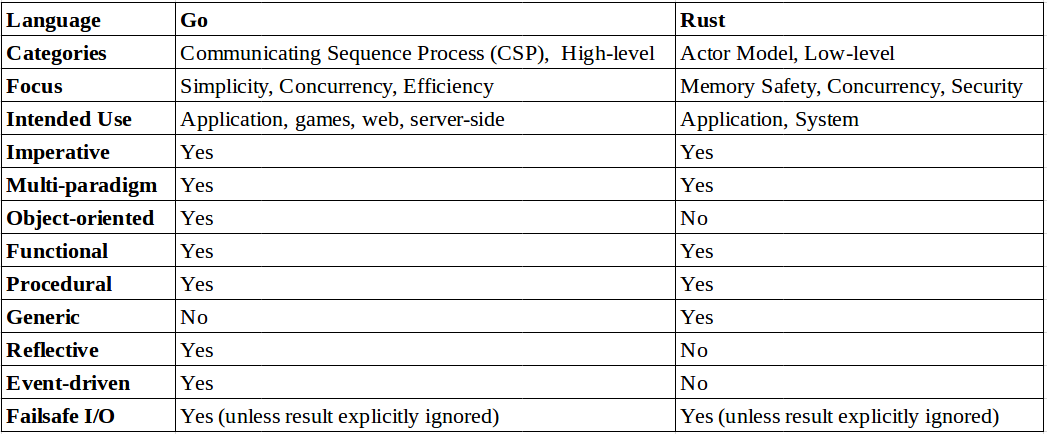
\includegraphics[width=1.0\textwidth]{Figure/go-vs-rust.png}
	\rule{35em}{0.5pt}
	\caption[Comparison of Go and Rust language characteristic]{Comparison of Go and Rust language characteristic}
\end{figure}

\subsection{Comparison of language categories and focus}

Go is a high-level language focus on simplicity, reliability and efficiency. The language is designed with communicating sequential process (CSP) to express concurrency based on message passing channels. The processes and messages communicate via goroutine and gochannel within a shared memory. \cite{go-csp} The language is intended to use for building web application programming interface (API) or networking application such as TCP or HTTP server to handle request.

Go possess simple syntax, garbage collector and runtime which allow developer to increase code readability and implement concurrency easier. However, Go is lack of language extensibility which leads to a limitation on implement manual memory management. \cite{go-problem}

\pagebreak

Rust is a low-level language focus on memory safety, security and fault tolerance. The language designed with actor model concurrent programming language that use “actors” as fundamental agent on message passing. The actor takes input, send output after performing functions. \cite{rust-actor-model} The processes and message communicate point-to-point via actors in a consistent state. The language intended use for system programmings such as building game engines, driver and embedded devices.

Rust doesn’t possess garbage collection and runtime which promote extensibility and deterministic on implement memory management. \cite{why-use-rust} However, Rust has much inherent complexity of syntax and semantics and has a high learning curve for a developer.
\pagebreak

\subsection{Similarities of Go and Rust language}

The similarities of both languages are discussed as follow: 

\begin{enumerate}[topsep=0pt,itemsep=-1ex,partopsep=1ex,parsep=1.5ex]
	
	\item \textbf{Imperative.} Go and Rust are imperative programming paradigm where a value can be assigned into a variable to perform operation on information located in memory. Moreover, these languages allow declaration of a variable to store the results in memory for later use, affect the global state of a variable.
	\item \textbf{Functional.} Go and Rust language can be written with mathematical functions to express control flow by combining function calls. The function avoid changing global state of variable. 
	\item \textbf{Procedural.} Go and Rust language can be written into statement structured and divided into function. The function known as procedure takes input processes it and produces output.
	\item \textbf{Multi-paradigm.} Go and Rust language are support various programming paradigm and provide developer to use suitable programming style to develop a program to achieve project objectives.
	\item \textbf{Failsafe I/O and callbacks.} Go and Rust language compiler warn error or throw an exception if the system calls fail. Go language throw errors if developer doesn’t use the declare function or variable and Rust language does not compile if found any dangling pointers.
	
\end{enumerate}
\pagebreak

\subsection{Difference between Go and Rust language}

The difference between both languages are discussed as follow: 

\begin{enumerate}[topsep=0pt,itemsep=-1ex,partopsep=1ex,parsep=1.5ex]
	
	\item \textbf{Object-oriented.} Go language support object-oriented programming with struct and interface. However, Rust is not an object-oriented language result of the idiomatic language and its appearance in an OO language. \cite{rust-not-oop}
	\item \textbf{Generic. } Go language is lack of generic where the compiler doesn’t allow declared a function or variable written in to-be-specified-later types await to be instantiated when needed for a specific purpose. However, Rust is possible to specify generalized function and avoid codes rewriting.
	\item \textbf{Reflective.} Go language possess the ability to observe and modify type, object, function execution on runtime by import “reflect”. However, Rust doesn’t have reflection.
	\item \textbf{Event-Driven. } Go is a high-level language enable write application respond to demand and expectation from mobile devices, multicore architectures and cloud computing environments. However,  Rust is a low-level language prevent the flow of program interrupt by an event from user actions to enforce security and safety. 
	
\end{enumerate}

\pagebreak

\section{Ubuntu 16.04.03 LTS 64-bit OS }

Ubuntu OS is an open source operating system with Linux distribution system and based on Debian architecture which provides long-term support (LTS) on security and fixes. \cite{difference-unix} The advantage of Ubuntu operating system are described below:

\begin{enumerate}[topsep=0pt,itemsep=-1ex,partopsep=1ex,parsep=1.5ex]
	
	\item \textbf{Free and customizable.} The openness of using Ubuntu OS offers a wide range of choices for the programmer to conduct development activities with Linux terminal. The APT packaging system allows developer to manage software and programming languages package efficient compared to Window operating system. The OS provides freedom in customization for a developer to catered different sets of need with source access and root permission to meet project requirements.
	\newline
	
	\item \textbf{Security.} The system files are owned by root in Ubuntu OS and not accessible by casual user, malware and third party software without root privilege. \cite{ubuntu-secure-than-window} As the operating system is maintained and contributed by vast amount of developer and programmer due to its open source and environment, the bugs are fixed efficiently with regular updates and provide less vulnerability for the attacker to exploit the system. \cite{linux-secure-than-window} The key factors underline within Ubuntu security provide sufficient statement to prove Ubuntu is more secure than Window or Mac OS on this project.	
	\newline
	
	\item \textbf{Consistent.} Ubuntu OS provide excellent consistent from front-end (UIUX) to back end. The user interface and user experience of Ubuntu operating system increase usability and efficiency in development, maintenance and deployment activities in the different version.
	\newline
	
	\item \textbf{Stable and Reliable.} UNIX preceded and outshine MS-DOS kernel with hardware abstraction, security model, resource management and various services that ran as background processes. \cite{difference-unix-msdos} Ubuntu promotes multitasking and multi-user which is suitable and ideal for this project to conduct concurrent and distributed processing activities with PostgreSQL. Last but not least, MS-DOS is an image loader system that preload memory addresses without memory or resource management quickly leads to BSOD and data corruption during data processing.
	
	
\end{enumerate}

\section{Debugging tools}

Debugging could be painful for a software engineer to monitor and identify the performance of applications running in concurrent and distributed on sophisticated operating systems like Ubuntu. 

Debugging with printf() for program bring many disadvantages and limitation during concurrency programming. The function could consume much memory in the multi-threaded environment because it’s not lightweight and thread safety. \cite{printf-bad} Moreover, it is not an efficient way to identify problems occurs related to memory allocation or interruption.

Therefore, debugger is used in this project to understand event or consequence happens in a running software system without consuming the enormous amount of memory. Simultaneously, it helps developer to save times on finding coding and logic errors in source codes.  \cite{what-is-tracing} 

\subsection{GDB Debugger}

GDB is a build in GNU debugger for UNIX systems to debug programs to obtain information of root cause that cause the program to fail. \cite{what-is-debugger} GDB allows set breakpoints and watchpoints on certain functions and print values during the program execution with terminal interface. Unfortunately, GDB possess limitation on finding bugs cause by memory leakage and compile errors.

\section{Eclipse for Parallel Application Developers Oxygen Release (4.7.0) IDE.} 

Eclipse is an integrated development environment create and maintain by Eclipse Open Source Project teams. The Eclipse Oxygen release possess better functionality and performance for a developer to manage, build and deploy software system. The advantage of Eclipse IDE are listed as follows: 

\begin{enumerate}[topsep=0pt,itemsep=-1ex,partopsep=1ex,parsep=1.5ex]
	
	\item \textbf{Auto Completion.} The openness of using Ubuntu OS offers a wide range of choices for the programmer to conduct development activities with Linux terminal. The APT packaging system allows developer to manage software and programming languages package efficient compared to Window operating system. The OS provides freedom in customisation for a developer to catered different sets of need with source access and root permission to meet project requirements.
	\newline
	
	\item \textbf{Integrated Environment. } The system files are owned by root in Ubuntu OS and not accessible by casual user, malware and third party software without root privilege. \cite{ubuntu-secure-than-window} As the operating system is maintained and contributed by vast amount of developer and programmer due to its open source and environment, the bugs are fixed efficiently with regular updates and provide less vulnerability for the attacker to exploit the system. \cite{linux-secure-than-window} The key factors underline within Ubuntu security provide sufficient statement to prove Ubuntu is more secure than Window or Mac OS on this project.	
	\newline
	
	\item \textbf{Debugger. } Ubuntu OS provide excellent consistent from front-end (UIUX) to backend. The user interface and user experience of Ubuntu operating system increase usability and efficiency in development, maintenance and deployment activities in the different version.
	\newline
	
	\item \textbf{Plugins.} UNIX preceded and outshine MS-DOS kernel with hardware abstraction, security model, resource management and various services that ran as background processes. \cite{difference-unix-msdos} Ubuntu promotes multitasking and multi-user which is suitable and ideal for this project to conduct concurrent and distributed processing activities with PostgreSQL. Last but not least, MS-DOS is an image loader system that preload memory addresses without memory or resource management quickly leads to BSOD and data corruption during data processing.
	
	
\end{enumerate}

\pagebreak

% MAIN SECTION ==============================
\section{Chapter Summary}

The finding for literature review is concurrent programming language possess specific built-in notation, package and functions to build parallel and distributed application. PostgreSQL is suitable for this project because it possesses MVCC that able handle concurrent request with good adaptivity and accuracy. Golang and Rust are concurrent programming language support multi-paradigm programming with multiprocessing and multithreading. Go language focused on simplicity while Rust language focuses on security. Both programming languages invented with different model and concepts for a different purpose.

Concurrent language is often compared and evaluated with configuration, categories and architecture to obtain performance and expressive power. The language's feature is essential to prove the performance of specific concurrent language. Debugging tools play a main role on observing processes and threads activities during the development and debugging activity to ensure program's execution is observed and error are discovered. 

 % LITERATURE SURVEY
\chapter{Project Design} 
% Main chapter title

\label{Chapter3} 
%Call reference to this2 chapter use \ref{ChapterX}

\lhead{Chapter 3. \emph{Project Design}} 
% Change X to a consecutive number; this is for the header on each page - perhaps a shortened title

\doublespacing
% LINE FORMATTING

%\clearpage
%\pagebreak

% MAIN SECTION =============================

\section{Phase 1}


\subsection{Introduction}
The primary focus of Phase 1 is implement prototype to prove theoretical concepts of the domain to research in this project. Requirements are listed as follow:

\begin{enumerate}[topsep=0pt,itemsep=-1ex,partopsep=1ex,parsep=1.5ex]

\item To acquire free large data set for big data processing.
\item To ensure data set acquired from the website are free, consent and clean with Devil Advocation Test. 
\item A program will be implemented in RUST and Go programming language as a proof-of-concept (POC) that CSV raw data is capable of importing into PostgreSQL database.
\item A program will be implemented with Go programming language as POC that PostgreSQL database transaction can be sequential and concurrent.
\item A program will be implemented with Go programming language as POC that reading CSV files can be sequential and concurrent.
\item To ease the debugging and troubleshooting on concurrent and distributed development environment, LTTng tracing network and Eclipse Trace Compass will be installed to obtain a reading and outputs traces via Common Trace File (CTF) binary format. 

\end{enumerate}

\pagebreak

\subsection{Data Collection}

The project is required to work with large data sets to utilize infrastructure and processing power of GO and RUST concurrent programming language. Data collection is conducted to identify of company recruitment preferences on higher education graduates of different subjects in the UK with basic company and LEO datasets. Data collected is required to be clean and able to solve interesting problem or question. 

The characteristic of free, consent and licensed data sets acquired from UK government website provider (data.gov.uk) are as follow:

\begin{table}[H]
	\resizebox{\textwidth}{!}{%
	\begin{tabulary}{1.0\textwidth}{|L|L|L|L|L|L}
		\hline
		{\bf No} & {\bf Name of Datasets}  						& {\bf Column } & {\bf Rows} & {\bf Size}	\\ \hline
		1.       & Longitudinal Educations Outcomes (LEO)       &  21          & 32706       & 1.8   GB		\\ \hline
		2.       & Basic Company Profile (Company)              &  55          & 3595702     & 667.5 MB		\\ \hline
		3.       & National Statistics Postcode Lookup (NSPL)   &  35          & 1754882     & 4.2	 MB		\\ \hline
	\end{tabulary}}
	\caption{Result of Golang programming on process CSV raw data}
\end{table}

The file format of all large dataset obtained are Comma Separated Values (CSV) format which the information is organized with one record as one line and each field is separated by comma (,). CSV format is used for data processing in this project because it is human readable and simple to be parse. It can be handle using PostgreSQL database and retrievable by programs. 

\pagebreak

\subsubsection{Longitudinal Education Outcomes (LEO) dataset }

The data set focus on employment and earnings outcome of Bachelor’s Degree graduate in Great Britain after five years. It contains information about students include personal characteristics, education or qualification achieved, employment and income earnings.  The data dictionary of longitudinal education outcome is created and placed in Appendix I.1.1.

\subsubsection{Basic Company dataset}

The data set possesses up-to-date basic companies information on UK register. It contains company names, annual returns filing dates, location details, account and basic information about mortgage and business changes. The data dictionary of basic company dataset is created and placed in Appendix I.1.2.

\subsubsection{National Statistics Postcode Lookup (NSPL) dataset}

\begin{figure}[H]
	\centering
	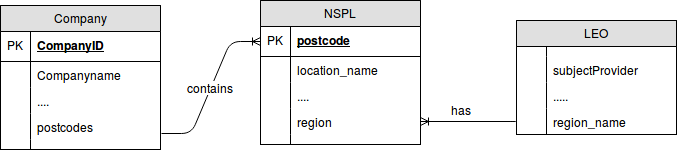
\includegraphics[width=0.9\textwidth]{Figure/erd-data.png}
	\rule{35em}{0.5pt}
	\caption[Entity Relationship Diagram]{Entity Relationship Diagram}
\end{figure}

As postcode data for every location on earth is unique. Company data sets possess \textbf{postcode} field in the business address, but LEO dataset do not have the \textbf{postcode} field which leads to difficulty of defining a relationship between these two datasets. Figure above show NSPL dataset serves as a linker to map \textbf{region} column from LEO data to link with \textbf{postcode} column found in company datasets.

The data set possesses current postcode for the United Kingdom. It contains information relates postcode number, location, country name, parliamentary constitution, electoral and other geographical details. The data dictionary of National Statistics Postcode Lookup (NSPL) dataset is created and placed in Appendix I.1.3.



\subsection{Data Validation}

\begin{figure}[H]
	\centering
	\includegraphics[width=1.0\textwidth]{FYP2/Chapter3/FYP2-data-validation-flowchart.png}
	\rule{35em}{0.7pt}
	\caption[Data Validation Procedure Flowchart]{Data Validation Procedure Flowchart}
\end{figure}

Data validation is conducted to inspect the quality dimension of data sources acquire in Data Collection (Section 3.1.2) to prevent corruption, inconsistency and conflicts during importing, using and processing. It is performed to ensure the data acquired are clean and in excellent quality. 

The important steps taken on validation of data are shown in Figure 3.5. The \textbf{completeness} of datasets will be examine to assures the characteristic of data fulfill Comma Separate Values (CSV) standard and requirement. The common test performed during data completeness check are using aggregate functions such as max, min or counts. \cite{data-completeness-check}

Furthermore, the \textbf{validity} of data types in each columns are measured to prevent incompatible data types during Data Importation, Object Relational Mapping (ORM) and Data Migration. The types of data stored in each columns of obtained datasets shall be identify to describe suitable data type for Database Definition Language (DDL) during database table creation. As an example, the alphanumeric and text field are usually defined as VARCHAR and field contains only number will be declared as INTEGER.  

In addition, the \textbf{uniqueness} of records will be verify to discover wasteful and duplication of data. The data redundancy indicates same piece of data are exist in multiple place. \cite{data-redundancy-definition} This condition will results in waste of space, data inconsistency and violates data integrity. If the duplication of data is discovered, database normalization will be performed to eliminate the duplication of records. 

Last but not least, the \textbf{consistency} of data will be analyze to ensure datasets obtained are conform to specific standards and meet requirements. The data consistency check shall be performed during data preparation to inspect discover missing, corrupted or invalid data in record. The conformity and consistency of data in specific column should be handled in wariness to prevent affect the outcomes and efficiency of data processing. If the data is found inconsistent, Data Cleaning and Data Importation will be conducted to fix the defects discovered in the datasets. 

\subsection{Performance Benchmarking}

To conduct a comparison between Go and RUST language, benchmarking plays an important role to achieve fairness in compare performance and expressive power of language.

The component that are benchmarked are listed below:  

\begin{enumerate}[topsep=0pt,itemsep=-1ex,partopsep=1ex,parsep=1.5ex]
	
	\item \textbf{SQL Queries run on program. } Go and Rust program execute the same amount of database retrieval query to achieve the fairness of comparison.
	\newline
	\item \textbf{Table configurations.} The space of table of this project should be same for Go and Rust program to test the performance. 
	\newline
	\item \textbf{Hardware configurations. } Both Go and Rust program are required to run on same hardware configuration to achieve fairness of comparison on performance.
	\newline
	
\end{enumerate}

\pagebreak

\subsection{Database Retrieval Program}

\subsubsection{Phase 1 System Context Diagram}

\begin{figure}[H]
	\centering
	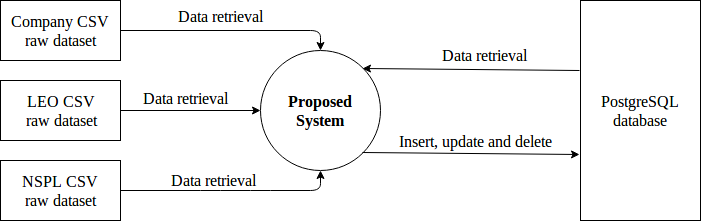
\includegraphics[width=0.9\textwidth]{Figure/fyp-context.png}
	\rule{35em}{0.5pt}
	\caption[Phase 1 System Context Diagram]{Phase 1 System Context Diagram}
\end{figure}

System context diagram provide high level view that defines relationship between proposed system with external entities. The proposed system is written in Go and Rust programming language with sequential and concurrent computing. The system shall process raw dataset stores in different nodes and dataset stores in PostgreSQL database. Moreover, the system should process data from raw CSV dataset and PostgreSQL database in sequential and concurrent manner. 

\subsubsection{Phase 1 Block Diagram}

\begin{figure}[H]
	\centering
	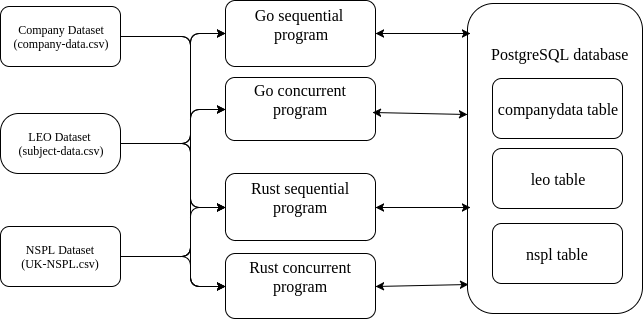
\includegraphics[width=0.9\textwidth]{Figure/block-diagram.png}
	\rule{35em}{0.5pt}
	\caption[Phase 1 Block Diagram]{Phase 1 Block Diagram}
\end{figure}

The block diagram provides a high-level overview of importation CSV into PostgreSQL with Go and Rust program. The large dataset store is store in different nodes with CSV format. Data stores in PostgreSQL database and raw CSV data at different nodes will be processed by Go and Rust program with sequential and concurrent manner. The database table is created with query in the terminal before Go and Rust program is executed.

\subsection{PostgreSQL Database Retrieval with Go and Rust program}

\subsubsection{Phase 1 Sequential Program Flowchart}

\begin{figure}[H]
	\centering
	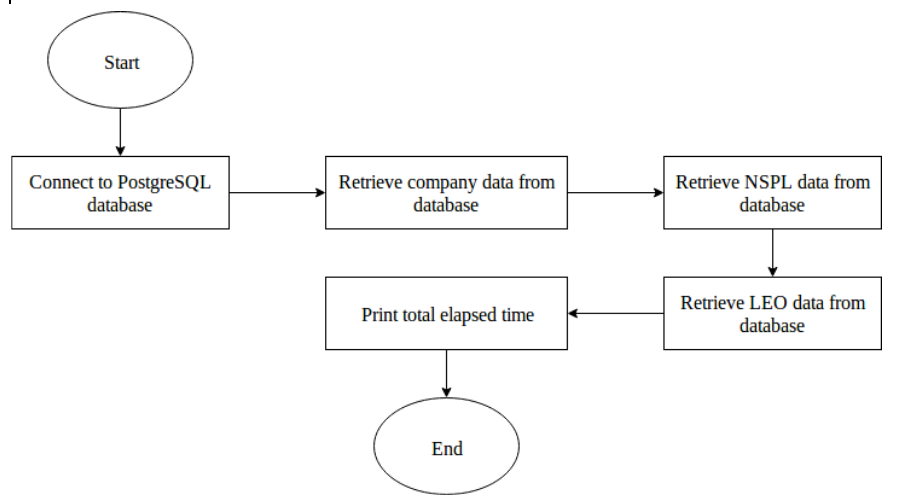
\includegraphics[width=0.9\textwidth]{Figure/postgres-data-sequential.png}
	\rule{35em}{0.5pt}
	\caption[Phase 1 Sequential program flowchart]{Phase 1 Sequential program flowchart}
\end{figure}

The flowchart provides a high-level view of concurrent manner during data retrieval in PostgreSQL with Go and Rust program. The program first establishes connection with PostgreSQL database with a connection string. Afterwards, it will retrieve a different set of data from various database table concurrently. The total elapsed time for entire program execution will be print.

\subsubsection{Phase 1 Concurrent Program Flowchart}

\begin{figure}[H]
	\centering
	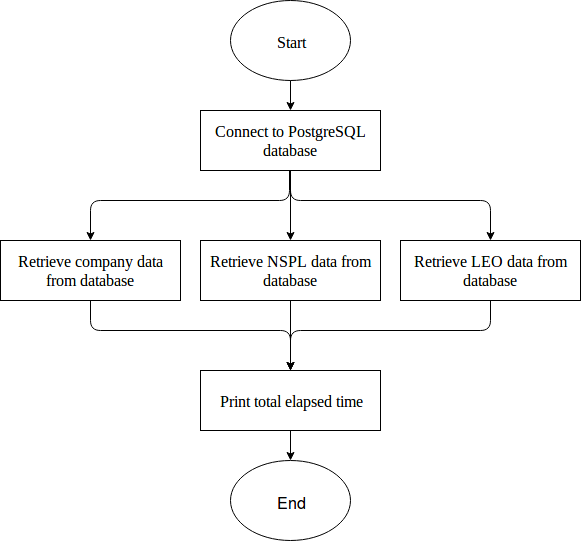
\includegraphics[width=0.9\textwidth]{Figure/postgres-data-concurrent.png}
	\rule{35em}{0.5pt}
	\caption[Phase 1 Concurrent program flowchart]{Phase 1 Concurrent program flowchart}
\end{figure}

The flowchart provides a high-level view on concurrent manner during data retrieval in PostgreSQL with Go and Rust program. The program first establish connection with PostgreSQL database with connection string. Afterwards, it will retrieve different set of data from different database table in concurrent manner. The total elapsed time for entire program execution will be print. 

\subsection{Raw CSV Data Retrieval with Go and Rust program}

\subsubsection{Phase 1 Sequential Program Flowchart}

\begin{figure}[H]
	\centering
	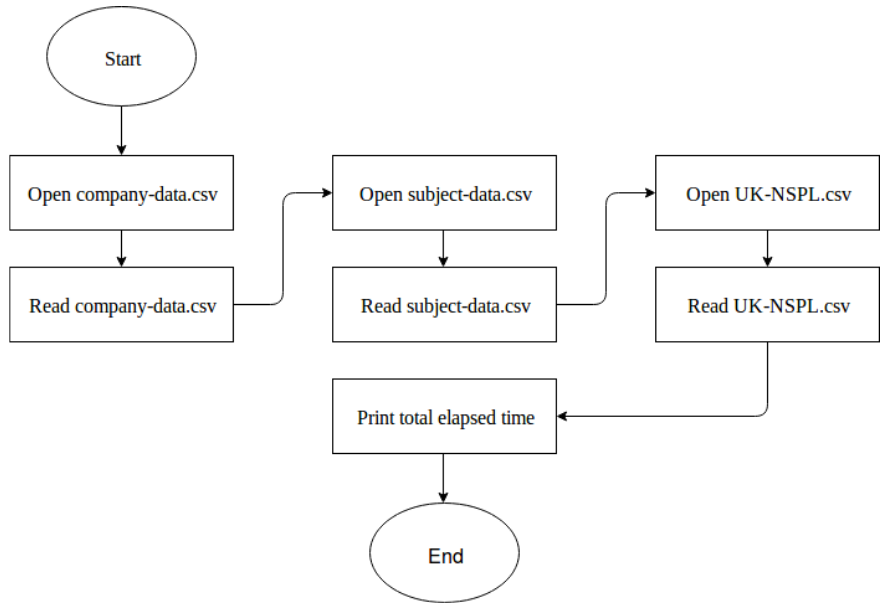
\includegraphics[width=0.9\textwidth]{Figure/seq-read-csv.png}
	\rule{35em}{0.5pt}
	\caption[Phase 1 Sequential program flowchart]{Phase 1 Sequential program flowchart}
\end{figure}

The flowchart provides a high-level view on sequential manner on reading CSV file with Go and Rust program. The program will open csv file and read containing data concurrently. The total elapsed time for entire program execution will be print.

\subsubsection{Phase 1 Concurrent Program Flowchart}

\begin{figure}[H]
	\centering
	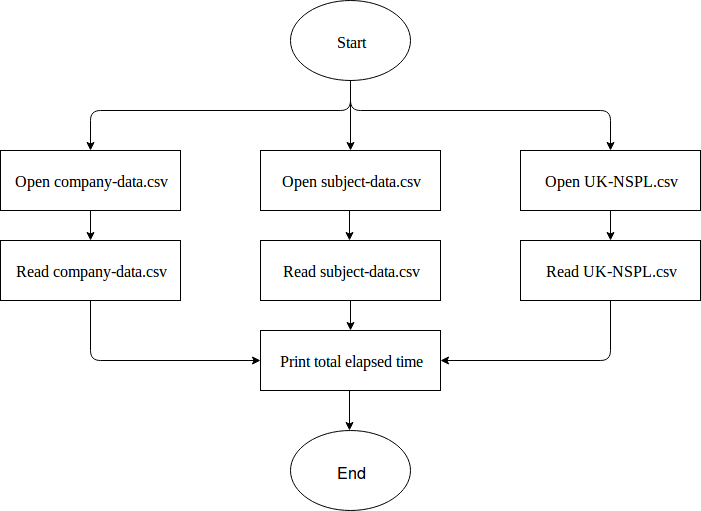
\includegraphics[width=0.9\textwidth]{Figure/concurrent-read-csv.png}
	\rule{35em}{0.5pt}
	\caption[Phase 1 Concurrent program flowchart]{Phase 1 Concurrent program flowchart}
\end{figure}

The flowchart provides a high-level view on concurrent manner on reading CSV file with Go and Rust program. The program will open csv file and read containing data in particular order of sequence. The total elapsed time for entire program execution will be print. 

\subsection{Proof of Concept in Phase 1}

\subsubsection{Phase 1 Deployment Diagram}

\begin{figure}[H]
	\centering
	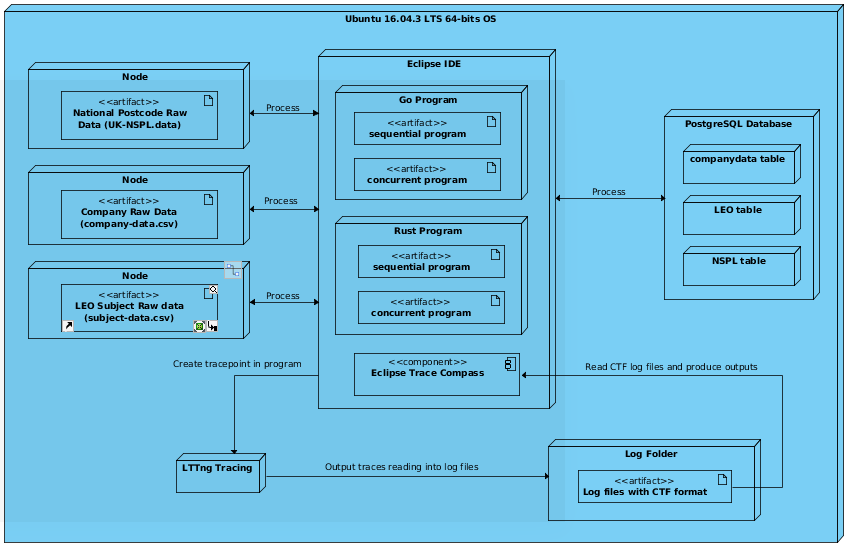
\includegraphics[width=1.0\textwidth]{Figure/dd-poc.png}
	\rule{35em}{0.5pt}
	\caption[Phase 1 Deployment Diagram]{Phase 1 Deployment Diagram}
\end{figure}

The deployment diagram describes the proof of concept of phase 1 in specification level and overall architecture of the project. Three database table is created in PostgreSQL database prepare to be processed. Simultaneously, three large data sets are stored in different nodes await to be process or retrieved. The Go and Rust program are written in sequentially and concurrently to process data from CSV file or PostgreSQL database system.

\section{Phase 2}

\subsection{Introduction}

Figure below shows Data Processing Cycle to provide an overview of activities carried out to process big data with the utilization of concurrent programming language and Structure Query Language (SQL).

\begin{figure}[H]
	\centering
	\includegraphics[width=1.0\textwidth]{FYP2/Chapter3/FYP2-data-process-cycle-flowchart.png}
	\rule{35em}{0.5pt}
	\caption[Data Process Cycle]{Data Process Cycle}
\end{figure} 

In Phase 2, we have established an extensive understanding on concurrent language characteristic by utilized the languages' feature on each activity in data processing cycle. The requirement as listed as follow: 

\begin{enumerate}[topsep=0pt,itemsep=-1ex,partopsep=1ex,parsep=1.5ex]
	
	\item Data encoding will be conducted with stream editor to convert dirty data into consistent format.
	\item Data transformation will be conducted to extracted data from CSV file and import into PostgreSQL database for data handling.
	\item Database normalization will be perform to eliminate data redundancy and improve data integrity.
	\item The structure of database schema and object (user and tables) will be created with scripts written in Data Definition Language (DDL) of PL/pgSQL (Procecural Language/PostgreSQL). 
	\item A \textbf{sequential} and \textbf{concurrent} program will be implemented with Go programming language as an Object Relational Mapping (O/R mapping tool) to convert raw data from CSV data sources into object model, the performance execution will be recorded and compared. 
	\item A \textbf{sequential} and \textbf{concurrent} program will be implemented with Go programming language as ORM tool to convert data retrieve from PostgreSQL database into object model, the performance execution will be recorded and compared.  
	\item A \textbf{sequential} and \textbf{concurrent} program will be implemented with Rust programming language as ORM tool to convert raw data from CSV data sources into object model, the performance execution will be recorded and compared. 
	\item A \textbf{sequential} and \textbf{concurrent} program will be implemented with Rust programming language as ORM tool to convert data retrieve from PostgreSQL database into object model, the performance execution will be recorded and compared.
	\item Data cleaning will be performed on CSV raw data to eliminate missing records and standardize the fields in common format. 
	\item Database tuning will be conducted to configure PostgreSQL database's environment for performance optimization on processing large-scale data and handling workloads. 
	\item A \textbf{sequential} and \textbf{concurrent} program will be implemented with Go programming language as data importation tool to export Company raw data from CSV data sources and import into PostgreSQL database. 
	\item Query tuning will be conducted to increase query execution performance on data processing. 
	\item Several \textbf{concurrent} program will be implemented with Go programming language as data migration tool to transfer company and NSPL data from legacy storage into normalized table within PostgreSQL database. 
	\item Data Manipulation Language (DML) scripts will be written with PL/pgSQL to transfer raw data from legacy storage into normalized table within PostgreSQL database.  
	\item Data verification will be conducted with UNIX command line to check the accuracy and consistency of database records after the data migration is complete. 
	
\end{enumerate}

\section{Data Encoding}

\subsection{Phase 2 Architecture Diagram}

\begin{figure}[H]
	\centering
	\includegraphics[width=1.0\textwidth]{FYP2/Chapter3/FYP2-data-encoding.png}
	\rule{35em}{0.5pt}
	\caption[Data Encoding Architecture Diagram]{Data Encoding Architecture Diagram}
\end{figure} 

Data encoding is a conversion of records or fields into specialized format for efficient transformation, importation and migration. \cite{data-encoding-definition} Figure 3.14 shows an architecture diagram that describe a high-level view of data encoding flow. The sed stream editor provide powerful feature to perform editing operations coming from a file to remove inconsistency data. \cite{sed-usage} 

The stream editor allow developer to make editing decisions by calling the commands on terminal. It consumes the dirty raw data as input file and perform text substitution line-by-line based on the text patterns of regular expressions provided in the commands. Ultimately, the encoded file will be output and store into the same directory. 

\section{Data Transformation}

\subsection{Phase 2 Architectural Diagram}

\begin{figure}[H]
	\centering
	\includegraphics[width=1.0\textwidth]{FYP2/Chapter3/FYP2-data-transformation-arc.png}
	\rule{35em}{0.5pt}
	\caption[Data Transformation Architectural Diagram]{Data Transformation Architectural Diagram}
\end{figure} 


Data transformation is the process of converting one format to another by extracting from source application into data warehouse. \cite{data-transformation-definition} 

Figure 3.15 shows the architectural diagram of data transformation process in this project. After the data inconsistency is eliminated with data encoding (performed in Section 3.3), the data in CSV format is extracted and import into PostgreSQL database with PL/pgSQL commands in terminal environment.

\section{Data Retrieval}

\subsection{Phase 2 Deployment Diagram} 

	\begin{figure}[H]
		\centering
		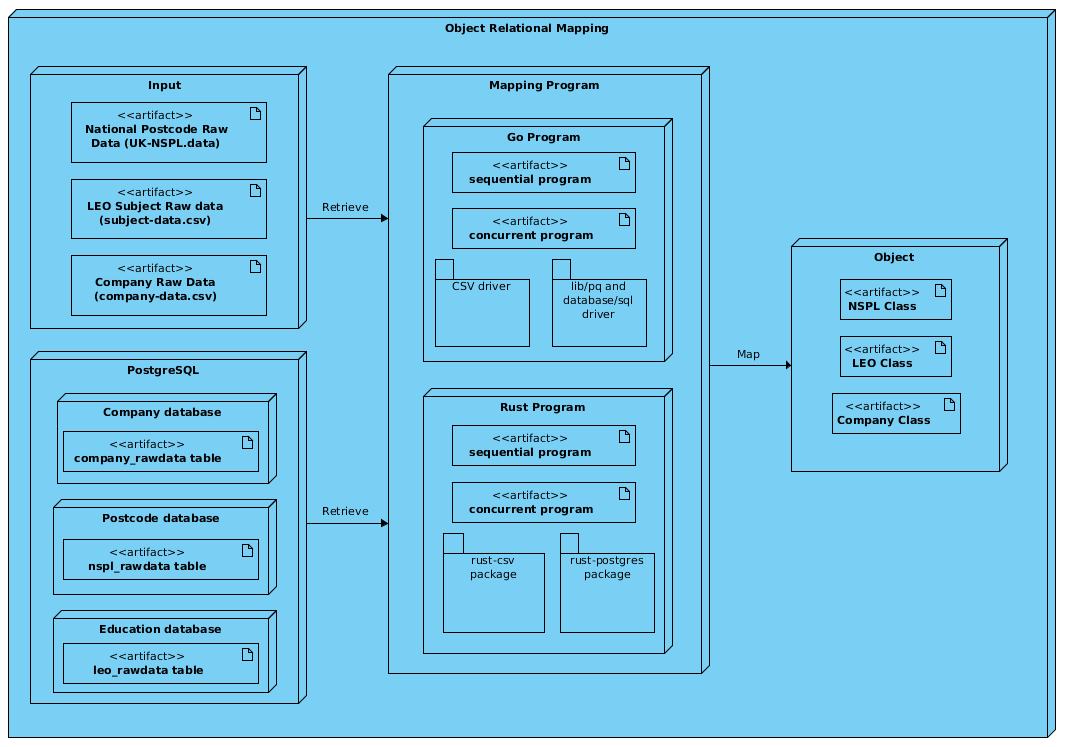
\includegraphics[width=1.0\textwidth]{FYP2/Chapter3/FYP2-ORM-deployment.png}
		\rule{35em}{0.5pt}
	\caption[Data Retrieval with ORM Deployment Diagram]{Data Retrieval with ORM Deployment Diagram}
	\end{figure}


Object-Relational Mapping (ORM) is a technique to manipulate data from database with object-oriented paradigm. The data retrieve from CSV data sources and PostgreSQL database will be convert into object model to ease the manipulation of data in discipline manner. \cite{orm-introduction} The approach increase usability, flexibility and improve data handling for Data Cleaning and Data Migration.

Figure 3.16 shows the ORM deployment diagram that provide graphic representation of mapping between object and data with mapping program written in Go and Rust programming language. In this project, we will construct our own ORM tools tool for data retrieval from CSV file and PostgreSQL database with the assistance of CSV package driver, PostgreSQL driver and built-in SQL library from respective language. 

All the rows of data will be retrieved from PostgreSQL database and CSV file with Go and Rust's ORM to conduct performance comparison between sequential and concurrent execution and concurrent programming languages' expressive power. The results will be recorded and compared. 

\section{Data Cleaning}

\subsection{Introduction}

Data cleaning is the action of detecting and removing missing, incomplete and data redundancy within database. \cite{data-cleaning-definition} The inconsistencies and incorrect records will be detected in the datasets obtained from the secondary sources because we have lack of control over the data quality. 

Data redundancy occurs within a data storage when same piece of data exists in two separate places or two different fields within a single database. Database without normalization will cause updation, deletion and insertion anomalies. The table below is used to understand these the impact of these anomalies on causing data inconsistencies. 

\begin{figure}[H]
	\centering
	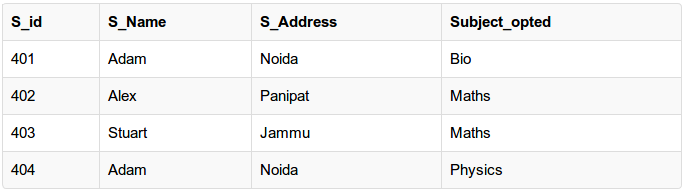
\includegraphics[width=1.0\textwidth]{FYP2/Chapter3/denormalization-example.png}
	\rule{35em}{0.5pt}
	\caption[Student table without normalization]{Student table without normalization}
\end{figure}

\begin{enumerate}[topsep=0pt,itemsep=-1ex,partopsep=1ex,parsep=1.5ex]
	
	\item \textbf{Insertion anomaly.} If student don't enroll any subject and \textbf{subject} is a mandatory field, the records cannot be insert into the database without the presence of other attributes or columns. 
	\item \textbf{Deletion anomaly.} If specific student willing to drop a subject, the entire records are forced to delete. As a result, certain attributes or part of the records are lost due to deletion of specific attributes without awareness which leads to missing data.
	\item \textbf{Updation anomaly.} To update student address in the table, the entire \textbf{address} column are required to be updated. If the duplicate records in the database are partially updated, it will leads to data inconsistency. 
	
\end{enumerate}

Therefore, \textbf{database normalization} and \textbf{data standardization} is conducted to improve the quality and reliability of the datasets.

\subsection{Database Normalization}

\subsubsection{Introduction}

Data normalization is conducted to eliminate data redundancy and improve data integrity. The mentioned method is an approach to remove all the data anomalies and recover the database into consistent state. \cite{normalization-benefits} Normalization is a multi-step approach and require rules to organize data into tabular forms and define relationships among them. The normalization rules and description are listed as follow: 

\begin{enumerate}[topsep=0pt,itemsep=-1ex,partopsep=1ex,parsep=1.5ex]
	
	\item \textbf{First Normal Form (1NF).} The rule required to eliminate repeating groups, identify primary key and discover \textbf{partial dependencies} or \textbf{transitive dependencies} among column by determine the determinant of the records. 
	\item \textbf{Second Normal Form (2NF).} The rule required to create new table with primary key assigned for \textbf{partial dependencies} elimination. 
	\item \textbf{Third Normal Form (3NF).} The rule required to create new table with primary key assigned for transitive dependencies elimination. 
	
\end{enumerate}

Relational database design is conducted to define entities, attributes, relationships and keys to fulfill normalization rules on eliminating data redundancy. The information contains in raw data are divided and separated into specific table and establish relationship among them to form an organized database. Ultimately, naming conventions and standards are used to form table to increase the usability and maintainability of database. 

\subsubsection{Phase 2 Normalized Company Entity Relationship Diagram} 

\begin{figure}[H]
	\centering
	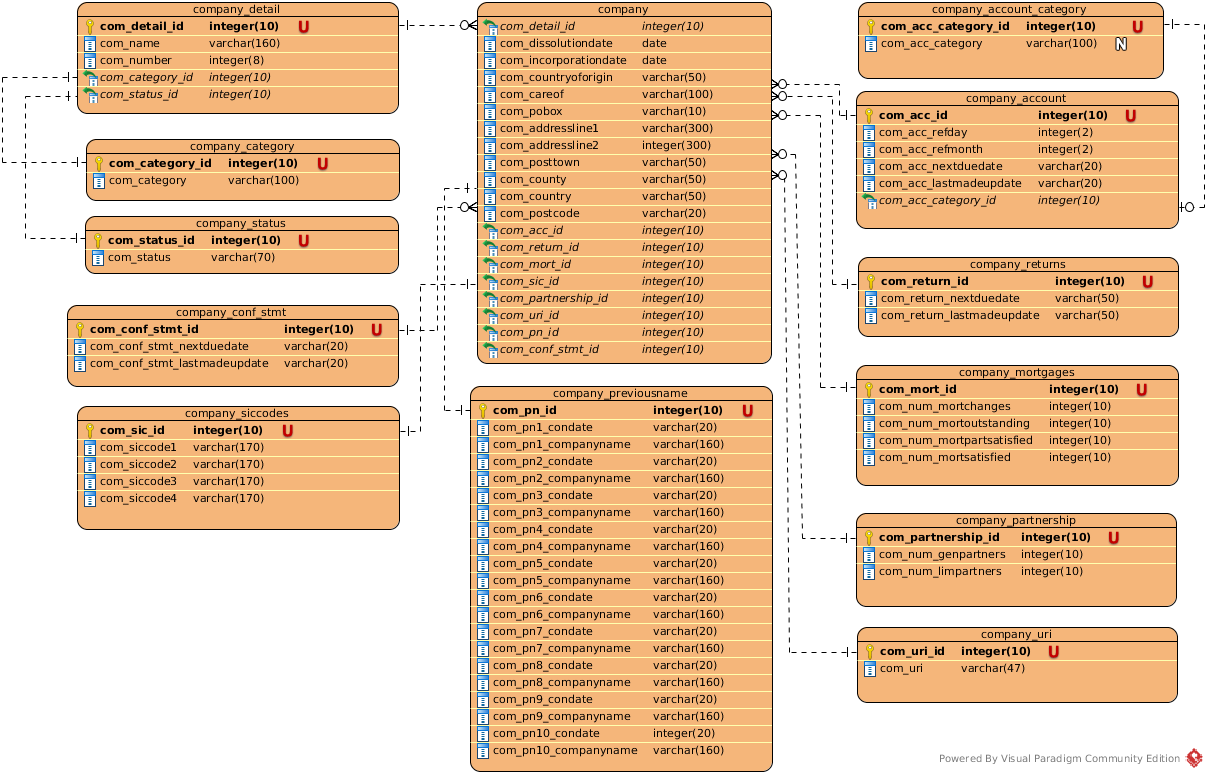
\includegraphics[width=1.1\textwidth]{FYP2/Chapter3/FYP2-Company-Normalized-ERD.png}
	\rule{35em}{0.5pt}
	\caption[Company Normalized Database Design]{Company Normalized Database Design}
\end{figure} 

The figure above shows Company's entity relationship diagram (ERD) to provide a graphical representation of normalized database design that display the relationships of entity stored in a database.

\subsubsection{Phase 2 Normalized Postcode Entity Relationship Diagram}

\begin{figure}[H]
	\centering
	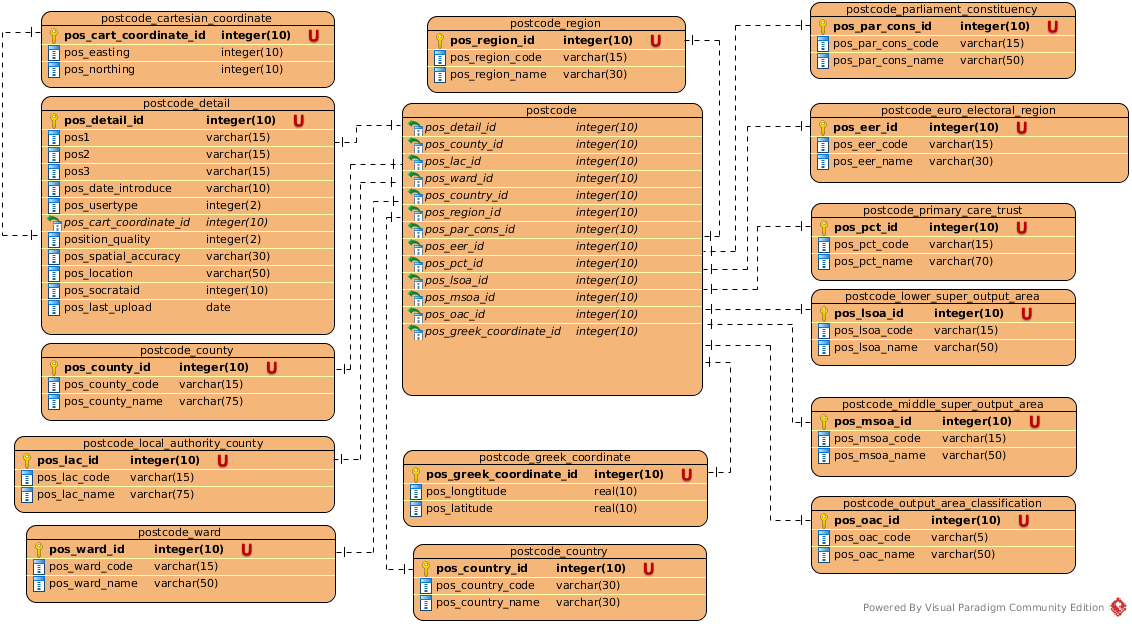
\includegraphics[width=1.1\textwidth]{FYP2/Chapter3/FYP2-Postcode-Normalized-ERD.png}
	\rule{35em}{0.5pt}
	\caption[Postcode Normalized Database Design]{Postcode Normalized Database Design}
\end{figure} 

The figure above shows Postcode's entity relationship diagram (ERD) to provide a graphical representation of normalized database design that display the relationships of entity stored in a database. 

\subsubsection{Phase 2 Normalized Education Entity Relationship Diagram} 

\begin{figure}[H]
	\centering
	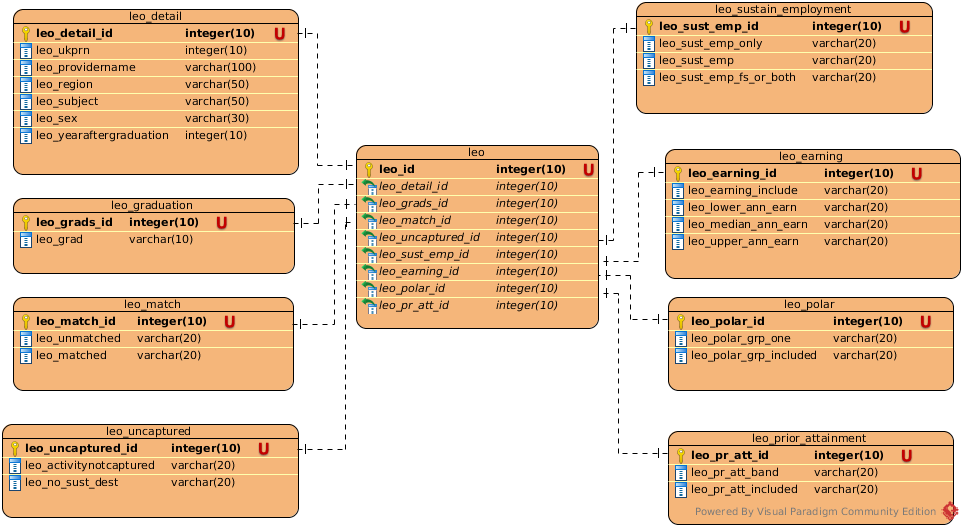
\includegraphics[width=1.1\textwidth]{FYP2/Chapter3/FYP2-Education-Normalized-ERD.png}
	\rule{35em}{0.5pt}
	\caption[Education Normalized Database Design]{Education Normalized Database Design}
\end{figure} 

The figure above shows Education's entity relationship diagram (ERD) to provide a graphical representation of normalized database design that display the relationships of entity stored in a database.

\subsection{Data Cleaning Parser}

\subsubsection{Phase 2 Company Data Cleaning Parser Deployment Diagram}

\begin{figure}[H]
	\centering
	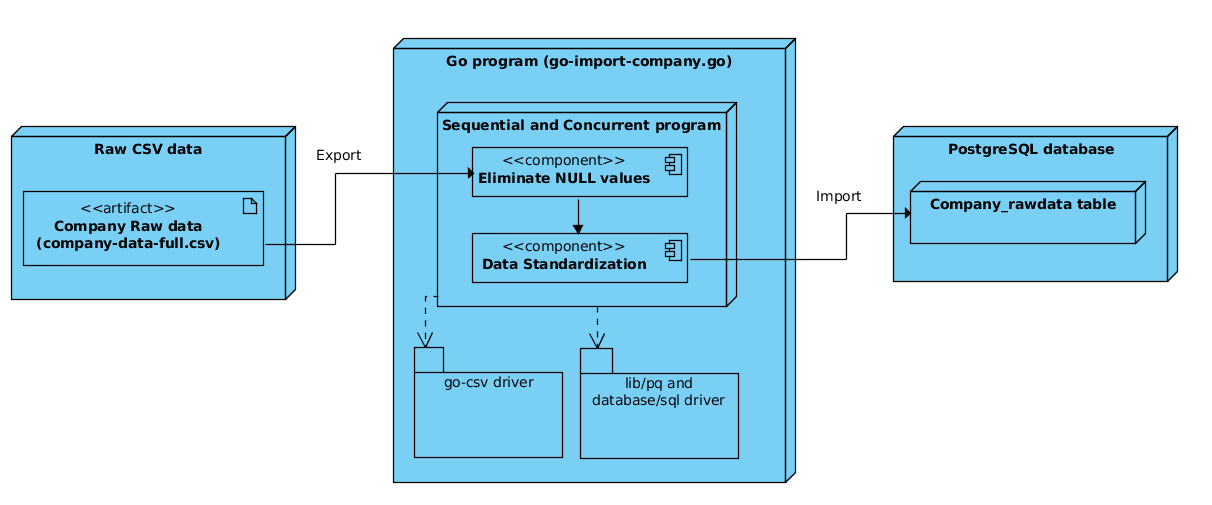
\includegraphics[width=1.0\textwidth]{FYP2/Chapter3/FYP2-data-cleaning-deployment.png}
	\rule{35em}{0.5pt}
	\caption[Company Data Cleaning Parser Deployment Diagram]{Company Data Cleaning Parser Deployment Diagram}
\end{figure} 

The figure 3.18 shows the deployment diagram of company data cleaning parser. 

The cleaning parser is written with Go program language that consume encoded company raw data (performed in Section 3.3) as input and make execution decisions to eliminate NULL values and perform data standardization to repair missing and incorrect data. Afterwards, the cleaned data will be stored into PostgreSQL database await to be processed. The program work similarly as ORM (mentioned in Section 3.5) by utilizing go-csv driver to retrieve data from CSV files and lib/pq or database/sql driver to establish connection and perform transaction with the PostgreSQL database. 

\section{Database Tuning}

\subsection{Phase 2 Database Tuning Flowchart}

\begin{figure}[H]
	\centering
	\includegraphics[width=0.65\textwidth]{FYP2/Chapter3/FYP2-database-tuning-flowchart.png}
	\rule{35em}{0.5pt}
	\caption[Database Tuning Flowchart]{Database Tuning Flowchart}
\end{figure} 

Database tuning is a process of configure PostgreSQL database's environment to optimize performance by increase throughput and decrease response time. The approach required to open PostgreSQL database configuration file with root access in Linux Operating System environment. The configuration made and reason to perform are describe as follow: 

\begin{enumerate}[topsep=0pt,itemsep=-1ex,partopsep=1ex,parsep=1.5ex]
	
	\item \textbf{Max Connection.} The number max connection of PostgreSQL database is modified to allow more \textit{Goroutines} from Go program to establish database connection concurrently and perform parallelize transaction. This modification helps increase performance on Data Cleaning and Data Migration in this project. If the connection pool is not modified, the database system will display FATAL error and terminate the process immediately. 
	\item \textbf{Shared Buffer.} The parameter of shared memory buffer shall be modified as 25 percents of memory in our systems. Increase the amount of memory PostgreSQL database uses for shared memory buffers allow the database to handle extra workloads. 
	\item \textbf{Shared Memory.} The maximum size of shared memory segment shall be modified to allow \textit{Goroutines} or \textit{threads} access to PostgreSQL database simultaneously for better data passing and avoid redundant copies. This configuration parameter determine dedicated memory for PostgreSQL to caching data and increase the space for threads to communicate with the database. The parameter shall be modify with Bytes(B). 
	
\end{enumerate}

Ultimately, restart of PostgreSQL database is required to update the changes and modifications. 

\section{Data Migration} 

Data migration is the process of transferring data within storage system for database migration. \cite{data-migration-definition} Data migration is extremely challenging as we need to take care of performance issues, data integrity, data consistency and prevent data corruption. The data should be protect carefully and prevent missing during the migration process. 

\begin{landscape}
	\subsection{Phase 2 Data Migration Deployment Diagram} 
	\begin{figure}[H]
		\centering
		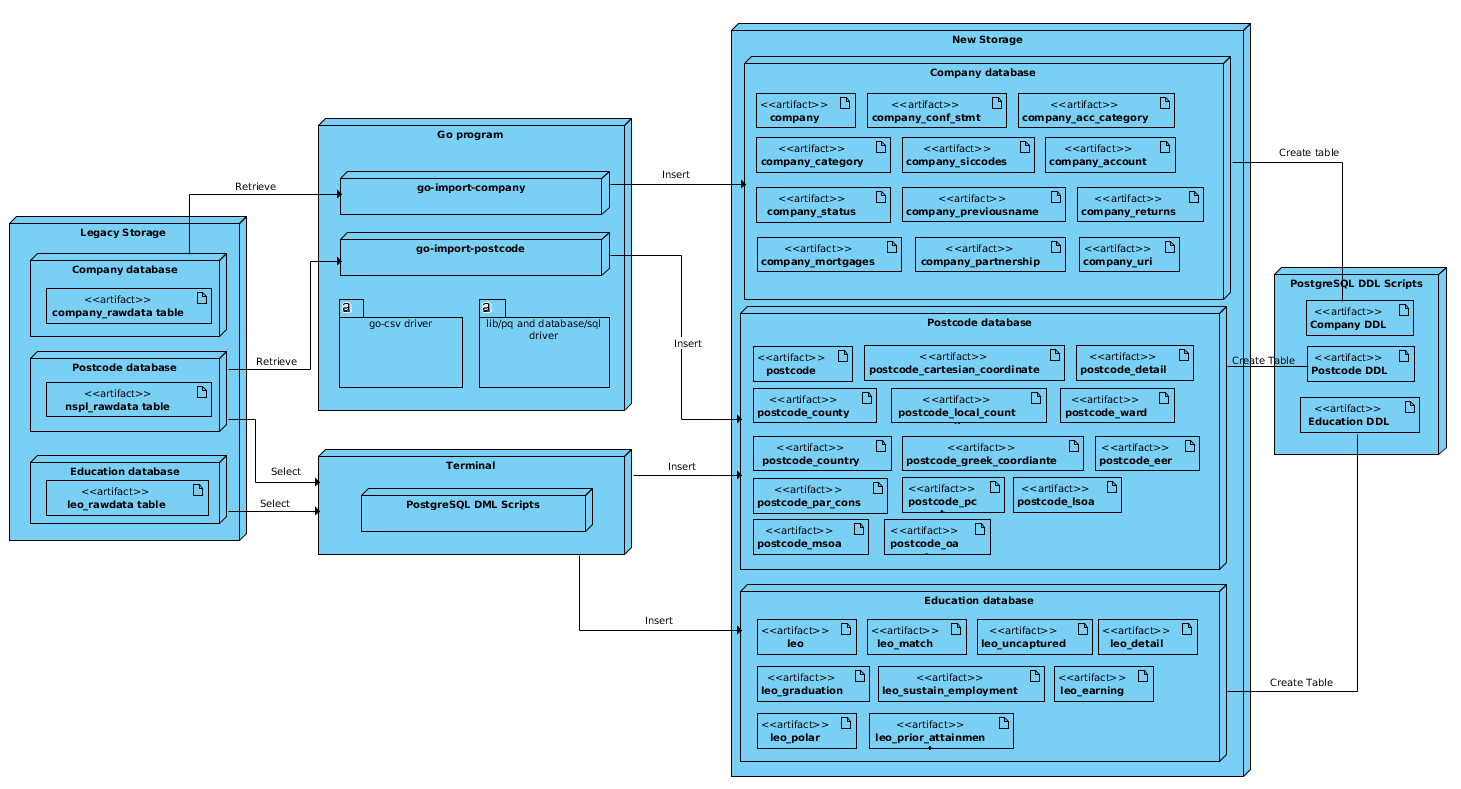
\includegraphics[width=1.4\textwidth]{FYP2/Chapter3/FYP2-data-migration-deployment.png}
		\rule{35em}{0.5pt}
		\caption[Data Migration Deployment Diagram]{Data Migration Deployment Diagram}
	\end{figure}
\end{landscape}

Figure 3.20 shows the deployment diagram of data migration process. 

The normalized table in all database are created with PL/pgSQL DDL scripts. Once the creation of table is successful, the data migration of education database is performed with PL/pgSQL DML script running in terminal environment. The mentioned database is migrated with script because it only contains 30000+ rows and its lightweight to be process with queries. 

Afterwards, the postcode and company database are migrated from legacy storage to new storage with the execution of scripts and Go program as shown in Figure 3.23. Both company and postcode data are migrated with Go program because it contains more than 4 millions rows in total and its difficult to handle with queries. The unique data is extracted from legacy storage and stored into the normalized table in new storage. 

The migration program is written with Go programming language with the inclusion of database/sql driver to establish connection and lib/pq driver to perform transaction with PostgreSQL database. All the migration process does not modify the source data in legacy storage to serve as backup for in case of emergence. In addition, the changes of migration can be easily tracked for verification purposes. Ultimately, the migration duration is recorded and measured.  


% MAIN SECTION ===============================
%\section{Chapter Summary}
%Your job here
 % Added PROJECT DESIGN
\chapter{Implementation Methodology} 
% Main chapter title

\label{Chapter4} 
%Call reference to this chapter use \ref{ChapterX}

\lhead{Chapter 4. \emph{Implementation Methodology}} 
% Change X to a consecutive number; this is for the header on each page - perhaps a shortened title

\doublespacing
% LINE FORMATTING

%\clearpage
%\pagebreak

% MAIN SECTION ==============================
\section{Software Engineering Methodology}

Software engineering life cycle (SDLC) is a well structured and iterative sequence of stages in to deliver quality research which meet or exceed project scope. It involves five major activities in this project which are: :

\begin{itemize}[topsep=0pt,itemsep=-1ex,partopsep=1ex,parsep=1.5ex]
	
    \item \textbf{Communication.} Student initiate the request to supervisor for apply specific project title offered in this semester. Requirement gathering is conducted in order to discuss the expectation of project and understand the critical factors to achieve project scope or objective. The process required mass amount of communication and collaboration between student and supervisor to ensure requirement are fully understood. 
      
    \item \textbf{Planning.} Project management plan is define and prepare with Gantt Chart to manage project execution by considering risk assessment, resources estimation, time and task management. The tools and techniques to be used requires to be understand in detail and comprehensive manner to achieve solid understand on whole project execution. 
           
    \item \textbf{Construction.} The creation of project documentation and program through a combination of verification, coding, writing, debugging and testing. The complexity of project are required to be minimize and reduce with the use of standards. The program is construct based on requirement designed in software design phase to ensure the outcomes meet project objectives. 
    
    \item \textbf{Testing.} The project outcomes and deliveries are required to update for supervisor and hand-in to the institution. Documentation and outcomes are required to conform with requirement specification and meet project requirements to ensure the project is doing right. 
    
\end{itemize}

\pagebreak

\subsection{Prototyping Model Method}

The software prototyping method is build prototypes with limited functionality as preliminary design to represent an approximation of concept. The prototype is implemented as proof of concepts for project objectives and reviewed by supervisor to enhance the prototype. 

Prototyping helps strengthen understanding the requirement of project through communication and negotiation. The characteristic and basic features of program are demonstrate to collect feedback for enhancement and improvement. This method helps improve familiarity and early determination of requirement specification before development process to reduce chances of fail in the project. Time and project resources can be estimated throughout the process to conduct task and time management in order to deliver the final product. 

\pagebreak

\section{Agile Software Methodology}

The process decision framework used by this project is Agile Methodology. The mentioned methodology simplified process decisions around incremental and iterative solution delivery, rapid deliver features and update in order to satisfy requirement for weekly project updates. Agile methodology provide flexibility for the project progress respond to change and modification from FYP weekly meeting.  

Agile software development describes set of principles for product and technology development under which requirements and solutions evolve through the collaborative effort of self-organizing management.  It advocates adaptive planning, evolutionary development, early delivery, and continuous improvement, and it encourages rapid and flexible response to change according to feedback provide by supervisor. The SDLC or paradigm involved in agile methodology in this project is Kanban. 

\pagebreak

\subsection{Kanban}

\begin{figure}[H]
	\centering
	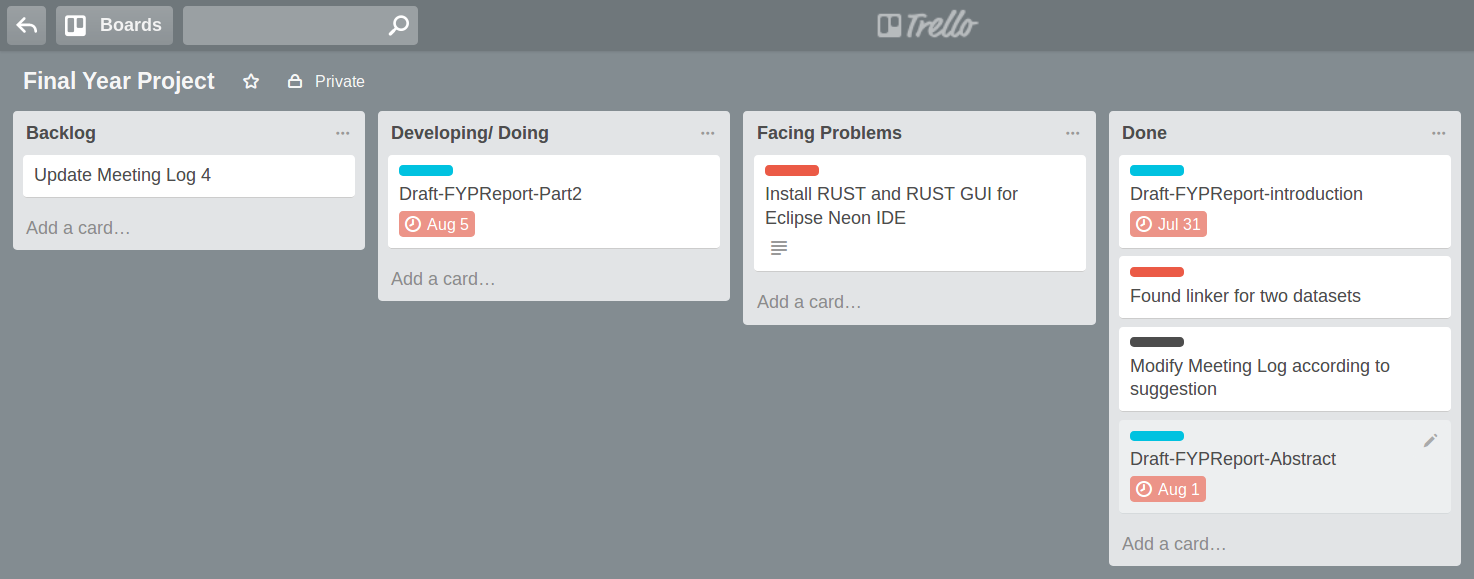
\includegraphics[width=1.0\textwidth]{Figure/kanban.png}
	\rule{35em}{0.5pt}
	\caption[Kanban board]{Kanban board}
\end{figure}

Kanban provide visual information of workflow by using sticky notes on a whiteboard to create a “picture” of our work. The board allow visualize the project development process or work flows within process and it helps ease the communicate status but also give and receive context for the work. Trello is used in this project as online Kanban board to manage the task in this methodology. 

There are an amount of work-in-progress (WIP) on each simple phased process to prevents overproduction and reveals bottlenecks dynamically to aware several roles whether are in bottlenecks. As an example, if the software pipelines are Backlog, Developing, Facing Problems and Done. There are WIP limits on each phased to increase the inspection and create awareness in order to facilitate adaptation based on the work loads. 

When a new requirement or changes requested, the task is insert into the backlog. The priority of the task are influenced by time constraint and importance. Afterwards, the task will be move into “developing” to began construction of documentation or codes. Once the task is encountered difficulty and problem, it will move to “”facing problem”. Alternatively, the task will move to “done” once the task is completed and ready to submit or show to supervisor during meeting. 

The Kanban events required to developed immediately and unknown incident may interrupt the progress depends on project feedback and requirement needs. A new high priority fix or changes may requested and it will break off the current project flow. Kanban allow the project respond to change efficiently and provide continuous update on progress to supervisor in order to submit quality works at end of project phase.  


\subsection{Methodology for this Project}

In this project, we will be developing Go and Rust program for conduct concurrent and distributed programming. To achieve the required tasks, rapid communication and modification is conducted to improve quality of program and satisfy project objectives. Prototyping method and Kanban will be use in this project.  

\pagebreak

%MAIN SECTION ================================
\section{Project Infrastructure}

\subsection{List of Hardware Resources}

\begin{enumerate}[topsep=0pt,itemsep=-1ex,partopsep=1ex,parsep=1.5ex]
\item \textbf{64-bit Personal Computer.} This machine is used for research and development activities of this project. The details are tabulated and shown below: 

\end{enumerate}

\begin{figure}[H]
	\centering
	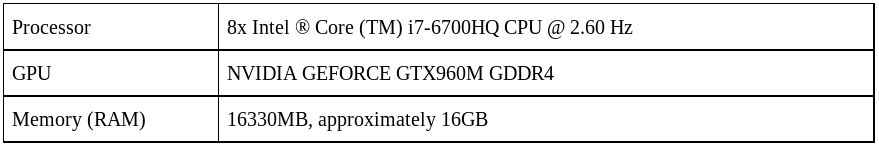
\includegraphics[width=1.0\textwidth]{Figure/computer-specs.png}
	\rule{35em}{0.5pt}
	\caption[Personal Computer Hardware table]{Personal Computer Hardware table}
\end{figure}

\subsection{List of Software Resources}

\begin{enumerate}[topsep=0pt,itemsep=-1ex,partopsep=1ex,parsep=1.5ex]

\item \textbf{Linux Ubuntu 16.04.3 LTS 64-bit.} The community driven and open source operating system is used to conduct concurrent and distributed computing with Go and Rust compiler installed. The details are discussed in Chapter 3.2.1. 

\item \textbf{Golang language compiler 1.8.3.} The linux amd64 gccgo compiler build Go source code into binary executable with “go build” and run the go program with “go run”. It is use to compile and run Go files this project.

\item \textbf{Rust language compiler 1.20.0. } The linux amd64 rustc compiler compile Go source code into executable with “rustc”.  It is use to compile Rust files in this project.

\item \textbf{PostgreSQL database 9.5.8.} The open source database management system is use for data handling and data storage for this project. The details are discussed in Chapter 3.2.3.

\item \textbf{Eclipse for Parallel Application Developers Oxygen Release (4.7.0) IDE.} The open source IDE provide perspective feature and integrated debugger to ease the coding and development activities for this project. The details are discussed in Chapter 3.2.2.

\item \textbf{Goclipse Plugin for Eclipse IDE.} The plugin provide debugging functionality, content assist, auto code indentation, open definition and integrated compiler for Go language on Eclipse IDE. 

\item \textbf{RUSTDT Plugin for Eclipse IDE.} The plugin provide syntax highlighting, error reporting, outline support, auto code indentation, debugging functionality and integrated compiler for Rust language on Eclipse IDE. 

\item \textbf{LTTng Tracing network. } The toolkits creating a tracepoint within Linux kernel, user application, libraries and output the traces into files. The details are discussed in Chapter 3.2.4.1.


\item \textbf{Eclipse Trace Compass.} The application view and analyze traces and produce useful graphical and tabulated information for debugging purposes. The details are discussed in Chapter 3.2.4.3.

\item \textbf{TeXstudio 2.10.8. } The software provide writing environment for create LaTeX document with numerous feature such as syntax-highlighting, reference checking with bibtex and various assistant. It is use for creating documentation for this project.
\pagebreak
\item \textbf{Visual Paradigm 14.1 free edition for non-commercial use.} The software is a free Unified Modelling Language Computer-Aided Software Engineering tool support 13 UML diagram types for software design and modelling. It is use to draw diagrams for this project. 

\end{enumerate}


\subsection{Other Project Resources}
\begin{enumerate}[topsep=0pt,itemsep=-1ex,partopsep=1ex,parsep=1.5ex]
	\item \textbf{Synaptic Package Manager. } The software system is a graphical package management program of APT libraries and provide same features as apt-get command. It provide great assist and help on managing software package dependencies. It is installed with \textit{“sudo apt-get install synaptic”} in terminal. 
	
	\item \textbf{Terminator.} Terminator provide multiple tabs, safe quit, UTF-8 encoding, automatic logging to ease the development activities for developer. The system is required to update source list with \textit{“sudo apt-get update”} and run \textit{“sudo apt-get install terminator”} to install the repository.
		
\end{enumerate}

\pagebreak

\subsection{Infrastructure Setup and Installation}

The required hardware and software resources are listed and discussed in Chapter 3.2, Chapter 4.2.1 and Chapter 4.2.2. 

\subsubsection{Go language compiler installation}

\begin{enumerate}[topsep=0pt,itemsep=-1ex,partopsep=1ex,parsep=1.5ex]
	\item Ensure Golang go1.8.3.linux-amd64.tar.gz is downloaded using wget in terminal. 
	\item Ensure downloaded file is extract, move and rename Golang directory. 
	\item Ensure Golang’s compiler export to system path. 
	\item Ensure Goroot and Gopath is set. 
	\item Ensure path to user profile .bashrc file is append. 
	\item Ensure Go executable and Go version installation is success. 
	\item Ensure Go libraries such as gocode, golint, guru, goimports, gorename and godef into Gopath directory are installed. 
	\item Ensure Godef Gometalinter is downloaded and executed. 
	
\end{enumerate}

The full installation steps for Go language compiler is found in Appendix A.1.
\pagebreak

\subsubsection{RUST language compiler installation}

\begin{enumerate}[topsep=0pt,itemsep=-1ex,partopsep=1ex,parsep=1.5ex]
    \item Install Rust toolchain with command line. 
    \item Export rust executable to system path. 
    \item Install Racer, Rustfmt, Rainicorn.
    \item Ensure all the required Rust executables are installed. 
	
\end{enumerate}

The full installation steps for RUST language compiler is found in Appendix A.2.

\subsubsection{Eclipse IDE installation}

\begin{enumerate}[topsep=0pt,itemsep=-1ex,partopsep=1ex,parsep=1.5ex]
    \item Ensure Java is installed before start download Eclipse.
    \item Run \textit{“sudo apt-get update”} and \textit{“sudo apt-get upgrade”} before start download. 
    \item Make eclipse-workspace folder as default storage for better management. 

\end{enumerate}

The installation details for Eclipse IDE is found in Appendix A.3.

\subsubsection{GoClipse plugin for Eclipse IDE installation}

\begin{enumerate}[topsep=0pt,itemsep=-1ex,partopsep=1ex,parsep=1.5ex]
	\item Install Goclipse plugin with Eclipse marketplace.
	\item Ensure Goclipse preferences and setting are correct.  
\end{enumerate}

The full installation steps for Goclipse plugin on Eclipse IDE is found in Appendix A.4.

\subsubsection{RustDT plugin for Eclipse IDE installation}

\begin{enumerate}[topsep=0pt,itemsep=-1ex,partopsep=1ex,parsep=1.5ex]
	\item Install RustDT plugin with Eclipse marketplace.
	\item Ensure RustDT preferences and setting are correct. 
\end{enumerate}

The full installation steps for RustDT plugin on Eclipse IDE is found in Appendix A.5.

\subsubsection{PostgreSQL database installation and setup}

\begin{enumerate}[topsep=0pt,itemsep=-1ex,partopsep=1ex,parsep=1.5ex]
	\item Install postgreSQL in command line. 
	\item Ensure database for FYP1 is created. 
	\item Create new user for database.
	\item Ensure database connection is established with user access.
\end{enumerate}

The full installation steps for PostgreSQL database is found in Appendix A.6.


% MAIN SECTION ===============================
%\section{Chapter Summary}
%Your job here
 % IMPLEMENTATION METHODOLOGY/PROPOSAL DESIGN
\chapter{Implementation Plan} 
% Main chapter title

\label{Chapter5} 
%Call reference to this chapter use \ref{ChapterX}

\lhead{Chapter 5. \emph{Implementation Plan}} 
% Change X to a consecutive number; this is for the header on each page - perhaps a shortened title

\doublespacing
% LINE FORMATTING

%\clearpage
%\pagebreak

\section{Project Task Identification}

\subsection{Identification of Critical Success Factors}

Critical success factors are a key requirement which is necessary and essential to be identified to achieve the project objectives in this project. The requirement for our design objectives are listed below: 


\begin{enumerate}
\item \textbf{Determine a suitable operating system.} The operating system should be reliable, secure and appropriate for data processing, concurrent and distributed computing activities. If the selected operating system does not meet requirements, a new operating system has to be considered.

\item \textbf{Acquire free public data set for big data processing.} Large data set is required for data processing with concurrent and distributed computing to make use of concurrent programming language’s package and architecture. If the data set obtains not clean and useful, data cleansing and data deduplication have to be conducted.

\item \textbf{Selection of database management system (DBMS). } The database-management system for this project should support for operating system, concurrent programming language and project activities. If the selected DBMS does not compatible and suitable, a new DBMS capability has to be considered. 

\item \textbf{Installation and setup DBMS for big data handling.} The selected database-management system should be installed and running on the operating system for data storing and data handling. The database system allows developer to conduct development activities for manage concurrency control for update and retrieval in this project.

\item \textbf{Selection of Go and RUST concurrent programming language for comparison. } There are many types of concurrent programming language for system development. The selected language for this project is RUST and Go. This programming language architecture, packages and capabilities should be considered to conduct performance comparison.

\item \textbf{Coding of “Import CSV into database” with Go program.} The program is required to write with Go language to read CSV and upload into PostgreSQL database. This task is conduct for data definition and data preparation before data processing is performed. 

\item \textbf{Coding of “Import CSV into database” with RUST program. } The program is required to write with Go language in order to read CSV and upload into PostgreSQL database. This task is conduct for data definition and data preparation before data processing is performed. 

\item \textbf{Conduct minor comparison on sequential and concurrent programming with Go and RUST language on PostgreSQL database transaction.} The sequential and concurrent program is required to write with Go and RUST language in order to conduct a comparison of execution time for database retrieval on PostgreSQL.

\item \textbf{Conduct minor comparison on sequential and concurrent programming with Go and RUST language on reading CSV files. } The sequential and concurrent program is required to write with Go and RUST language to conduct a comparison of execution time on reading CSV files.

\item \textbf{Installation of LTTng tracing network on user application or Linux kernel to produce outcomes into log files. } The open source software tracing toolkits enable the developer to create a tracepoint in Linux kernel or user applications to obtain process reading and create output into log files as Common Trace Format (CTF). This task has to be completed to improve troubleshooting and debugging process.

\item \textbf{Install Eclipse Trace Compass to extract and read Common Trace Format information from log files. } The open source Eclipse IDE plugin read CTF files and produce useful graphical and tabulated information from traces. This task has to be completed to improve debugging process and analyse process behaviour.

\end{enumerate}

\pagebreak

\subsection{Project Tasks for FYP Phase 1}

\begin{enumerate}[topsep=0pt,itemsep=-1ex,partopsep=1ex,parsep=1.5ex]
	
\item Installation of Ubuntu 16.04 LTS 64-bit operating system.
\item Acquire free public data set for big data processing.
\item Installation of  Eclipse Parallel Application IDE Parallel Oxygen version. 
\item Selection of Go and RUST concurrent programming language for comparison.
\item Installation of Go language compiler and Goclipse plugin for Eclipse IDE.
\item Installation of RUST language compiler and RustDT plugin for Eclipse IDE.
\item Selection of PostgreSQL object-oriented relational database management system (OORDBMS).
\item Installation and setup PostgreSQL database system intro PC for data handling.
\item Golang programming for import CSV files into PostgreSQL database.
\item Sequential and concurrent programming with Golang on PostgreSQL database retrieval.
\item Sequential and concurrent programming with Golang on reading CSV files.
\item Big data checking, cleaning and preparation with Devil Advocate. 
\item Installation of LTTng tracing network on user application or linux kernel.
\item Install Eclipse Trace Compass to extract and read Common Trace Format information from log files.

\end{enumerate}

\begin{landscape}
	\subsection{Gantt Chart for Phase 1}
	\begin{figure}[H]
		\centering
		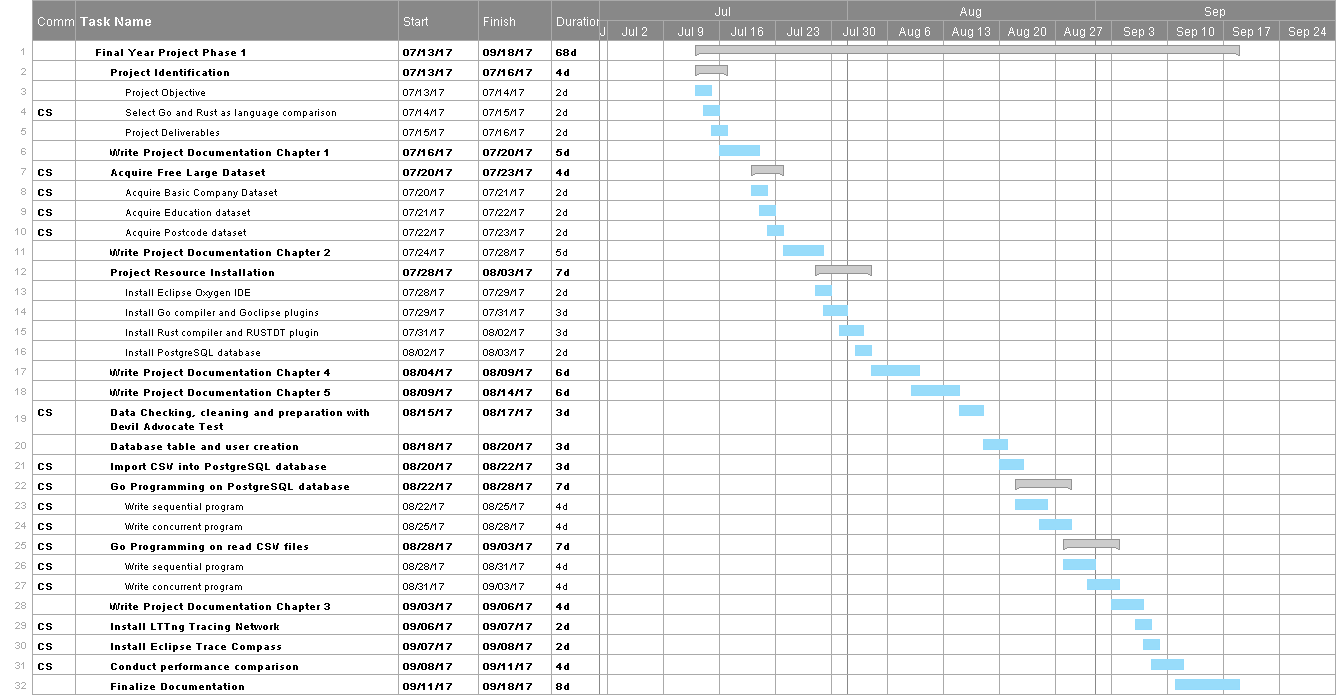
\includegraphics[width=1.5\textwidth]{Figure/Gantt1.png}
		\rule{35em}{0.5pt}
		\caption[Gantt Chart for Phase 1]{Gantt Chart for Phase 1}
	\end{figure}
\end{landscape}

\subsection{Project Tasks for FYP Phase 2}

\begin{enumerate}[topsep=0pt,itemsep=-1ex,partopsep=1ex,parsep=1.5ex]
	\item Data encoding.
	\item Data transformation. 
	\item Data parsing. 
	\item Data cleansing. 
	\item Data normalization.
	\item Database tuning. 
	\item Query tuning. 
	\item Data migration.
	\item Sequential and concurrent programming with Go and RUST on PostgreSQL database retrieval.
	\item Sequential and concurrent programming with Go and RUST on reading CSV files.
	
\end{enumerate}

\begin{landscape}
	\subsection{Gantt Chart for Phase 2}
	\begin{figure}[H]
		\centering
		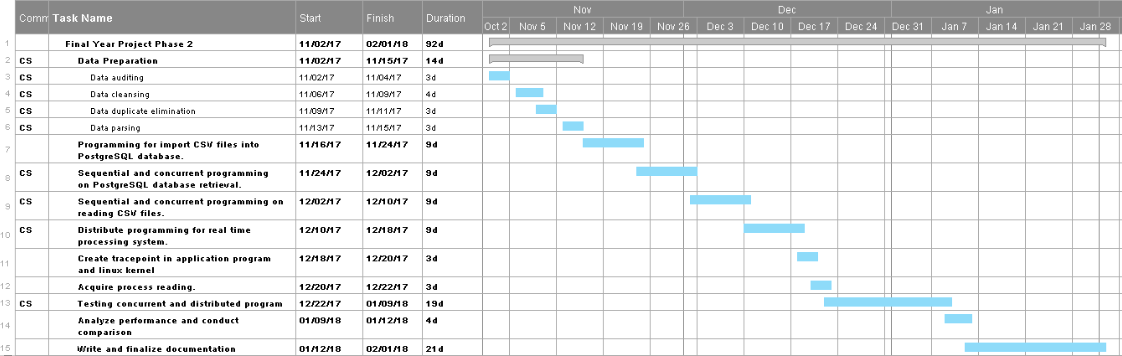
\includegraphics[width=1.5\textwidth]{Figure/Gantt2.png}
		\rule{35em}{0.5pt}
		\caption[Gantt Chart for Phase 2]{Gantt Chart for Phase 2}
	\end{figure}
\end{landscape}


\subsection{Milestone Deliverables}
The milestone deliverables are:

\begin{enumerate}[topsep=0pt,itemsep=-1ex,partopsep=1ex,parsep=1ex]
\item Go program for data parsing, object relational mapping and data migration. 
\item RUST program for data parsing and object relational mapping.
\item PL/pgSQL's DDL, DML and DCL scripts for database creation, manipulation and migration control.
\item A report based of this project. 
\end{enumerate}

%MAIN SECTION ================================
\section{Planned Execution Activities}

\subsection{Phase 1}

\begin{enumerate}[topsep=0pt,itemsep=-1ex,partopsep=1ex,parsep=1.5ex]
	
	\item \textbf{Data Validation.}
	 The Data Validation is conducted to ensure obtained raw CSV data set is clean and useful. The expected result of this test is the number of commas in the record should not exceed the number of columns in a database. In addition, the data content itself should be unique and suitable for storing in the database. More information is provided in Appendix B.1.
		
	\item \textbf{Golang programming for import CSV files into PostgreSQL database.}
	The Golang programming for import CSV raw data into PostgreSQL is to ensure Go language is capable of processing raw CSV data and PostgreSQL database. The expected result for this program should read 100 rows of data from raw CSV file and insert into PostgreSQL database. More information is provided in Appendix C.
	\pagebreak
	
	\item \textbf{Sequential and concurrent programming with Golang on PostgreSQL database retrieval.}
    The Go program should retrieve 300 rows of data from three tables (each table 100 rows) in PostgreSQL database sequentially and concurrently. The expected result for this program is concurrent processing should have better performance than sequential. More information is provided in Appendix D.	
	
	\item \textbf{Sequential and concurrent programming with Golang on reading CSV files.}
	The Go program should retrieve 100 rows of data from raw CSV file sequentially and concurrently. The expected result for this program is concurrent processing should have better performance than sequential. More information is provided in Appendix E.
	 
\end{enumerate}

\subsection{Phase 2}

\begin{enumerate}[topsep=0pt,itemsep=-1ex,partopsep=1ex,parsep=1.5ex]
	
	\item \textbf{Data encoding.}
	This activity is a deliverable of Phase 2 in this project. It is conducted to ensure that the dirty and corrupted datasets are converted into consistent format so that it will be safe to used for Object Relational Mapping, Data Transformation and Data Parsing. 
	
	\item \textbf{Development of PL/pgSQL scripts for data transformation.} 
	This activity is a deliverable of Phase 2 in this project. It is conducted to extract data in CSV format from raw datasets and import into PostgreSQL database. 
	
	\item \textbf{Development of Go and Rust Object Relational Mapping (ORM) program for data retrieval.}
	This activity is a deliverable of Phase 2 in this project. The data from CSV file and PostgreSQL database are retrieved and map into object model. Go and Rust program should retrieve 4 millions row of data from raw CSV file and PostgreSQL database in sequential and concurrent manner. The execution duration of each program are tabulated and recorded for comparison purposes. 
	
	\item \textbf{Development of PL/pgSQL DDL scripts for normalized entity creation.}
	This activity is a deliverable of Phase 2 in this project. It can eliminate redundancy and data anomalies to improve data integrity. Database design is performed to define table and establish relationship between entity to create a relational database schema. Moreover, normalized table will be created correctly with PL/pgSQL's DDL scripts based on the Entity Relationship Diagram shown in Section 3.
	
	\item \textbf{Development of Go data parser program.}
	This activity is a deliverable of Phase 2 in this project. The missing fields will be eliminated and data standardization is conducted to promote conformity and usability of data. 
	
	\item \textbf{Database tuning.}
	This activity is a deliverable of Phase 2 in this project. It is performed to configure PostgreSQL's database environment and setting to increase performance on data processing. 
	
	\item \textbf{Query tuning.}
	This activity is conducted to optimize database transaction performance and avoid poor performance execution on data processing activities. 
	
	\item \textbf{Development of PL/pgSQL's DML, DCL scripts and Go concurrent program for database migration.}
	This activity is a deliverable of Phase 2 in this project. The data that are transformed and cleaned will be import into normalized table. These data are migrated from legacy storage into new storage within PostgreSQL database. 
	
\end{enumerate}

 % IMPLEMENTATION PLAN
\chapter{Results and Findings} 
% Main chapter title

\label{Chapter6} 
%Call reference to this chapter use \ref{ChapterX}

\lhead{Chapter 6. \emph{Results and Findings}} 
% Change X to a consecutive number; this is for the header on each page - perhaps a shortened title

\doublespacing
% LINE FORMATTING

%\clearpage
%\pagebreak

% MAIN SECTION ==============================

\section{Phase 1}

\begin{enumerate}[topsep=0pt,itemsep=-1ex,partopsep=1ex,parsep=1.5ex]
	
	\item \textbf{Data validation.}
	This activity has been successfully achieved. It has been found the method can detect unmatched numbers of commas, unsuitable data types during data importation from CSV to PostgreSQL database and identify the uniqueness of rows and columns in data. Results and detailed information is provided in Appendix B.2 to B.4.
	
	\item \textbf{Golang programming for import CSV files into PostgreSQL database.}
	This activity has been successfully achieved. The program is capable to read 100 rows of data from three datasets and import into PostgreSQL database. Results and detailed information is provided in Appendix H.
	
	\pagebreak
	
	\item \textbf{Sequential and concurrent programming with Golang on PostgreSQL database retrieval.}
	This activity has been successfully achieved. The program is capable to prove concurrent processing is faster than sequential in data retrieval with PostgreSQL database. Results and detailed information is provided in Appendix G.
	
	\item \textbf{Sequential and concurrent programming with Golang on reading CSV files.}
	This activity has been successfully achieved. The program is capable to prove concurrent processing is faster than sequential in reading CSV data. Results and detailed information is provided in Appendix F.
	
\end{enumerate}

\section{Phase 2}

\begin{enumerate}[topsep=0pt,itemsep=-1ex,partopsep=1ex,parsep=1.5ex]
	
	\item \textbf{Data encoding.} This activity has been successfully achieved. The dirty and corrupted CSV raw datasets can be converted into consistent format with stream editor. Result and detailed information is provided in Appendix J.3.
	
	\item \textbf{Development of PL/pgSQL scripts for data transformation.} This activity has been successfully achieved. The developed scripts is capable to extract data from CSV format from raw datasets and import into PostgreSQL database. Result and detailed information is provided in Appendix K.3.
	
	\item \textbf{Development of Go and Rust Object Relational Mapping (ORM) program for data retrieval.} This activity has been successfully achieved. The Go and Rust program developed is capable to retrieved data from CSV file and PostgreSQL database and map into object model in sequential and concurrent manner. The activity proves concurrent processing is faster than sequential in data retrieval with PostgreSQL database and reading CSV data. Moreover, it proves Go programming languages possess faster processing time compared to Rust programming languages. Result and detailed information is provided in Appendix Q.
	
	\item \textbf{Development of PL/pgSQL DDL scripts for normalized entity creation.} This activity has been successfully achieved. The database design is capable to define table and establish relationship between entity. In addition, the PL/pgSQL's DDL scripts developed is able to create database entity based on the database design correctly. Result and detailed information is provided in Appendix M.4.
	
	\item \textbf{Development of Go data parser program.} This activity has been successfully achieved. The developed Go program is capable to eliminate NULL values and standardize the records of specific columns to promote conformity and usability of data. Result and detailed information is provided in Appendix N.2. 
	
	\item \textbf{Database Tuning.} This activity has been successfully achieved. The number of database maximum connections, amount of shared buffer utilized and maximum of shared memory segments are configured to increase performance and transaction efficiency of concurrent program. Result and detailed information is provided in Appendix O. 
	
	\item \textbf{Development of PL/pgSQL's DML scripts and Go concurrent program for database migration.} This activity has been successfully achieved. The PL/pgSQL's DML, DCL scripts is capable to retrieve unique data from legacy storage and insert into normalize table. In addition, the scripts and Go program are capable to migrate more than 4 millions row of data into normalized table without causing missing of records. Result and detailed information is provided in Appendix P.3 and P.4. 
	
\end{enumerate}

 % RESULTS AND FINDINGS
\chapter{Comparison Discussion and Recommendations} 
% Main chapter title

\label{Chapter7} 
%Call reference to this chapter use \ref{ChapterX}

\lhead{Chapter 7. \emph{Comparison Discussion and Recommendations}} 
% Change X to a consecutive number; this is for the header on each page - perhaps a shortened title

\doublespacing
% LINE FORMATTING

%\clearpage
%\pagebreak

% MAIN SECTION ==============================

\section{Problems Encountered \& Overcoming Them}

\subsection{Acquisition of free large datasets for data processing}

The problem encountered during data gathering of this project is difficulty on finding suitable free big data from websites. It is a challenge to find problem and raise question by going into data details. It took huge amount of time to understand the focus of project and gather desired data for problem solving. 

With the help of supervisor, I had successfully obtained suitable datasets for this project. He provides guidance and helping hand to clear my doubts and confusion by suggests several website and introduce various data repositories during the meeting. 

\subsection{Goclipse plugin compile error}

Eclipse IDE could not compile and build my Go files, this is because the IDE couldn’t find GOROOT in usr/local/go. The development activities cannot proceed and face impediment on executing critical success factors. The cause of the problem is Golang compiler executable doesn't possess a copy in usr/local/go, which caused Eclipse fail to compile Go file because couldn't file the compiler. 

The problem is resolved with help of supervisors, he guides me to execute Linux command line to resolve the problem during FYP meeting. Moreover, he helps identify the root cause of problem with Google Hangout in the midnights. 

\subsection{Unclear and doubts on writing documentation}

The problem encountered during writing documentation is unclear about the purpose and objectives of each section which leads to messy and poor content deliveries in writing. A certain standard and requirement should be achieved in writing the FYP document.

The problem is resolved with the help of supervisor as he patiently guide us to arrange the content layout of document and writing citation with references.  

\subsection{Difficulty on understand concurrent programming concepts}

The problem encountered during coding process is to understand concurrent concepts. It took an enormous amount of time to implement the ideas of Goroutine and Go channel into the program to achieve concurrency with Go programming language. This is because I do not possess the experiences and knowledge to build a concurrent program.

The problem is resolved with the help of official documentation and StackOverflow websites which provide clear explanation and enlightenment for me to understand the concepts and semantics of languages. 

\subsection{Difficulty on develop PG/pgSQL scripts on data migration.}

The problem encountered during development process is writing PG/pgSQL scripts to perform data migration. The DML query requires to use \textit{insert with select} query to retrieve primary key from each entity and insert as foreign key into specific table. In addition, the query is shall possess high throughput on data processing while maintaing the data consistency and validity during the migration process. The mentioned difficulty has caused impediment on development progress and stuck for a week. 

The problem is posted on Stackoverflow forum as database question and it was discussed by various database expert with high reputation in the community. Ultimately, the issue is resolved with suggested answer provided and the query with JOIN works on my project.

\subsection{Difficulty on perform database tuning.}

The problem encountered during database tuning are listed as follow: 

\begin{enumerate}[topsep=0pt,itemsep=-1ex,partopsep=1ex,parsep=1.5ex]

	\item \textbf{Understand the risk of modification. } Modified number of maximum concurrent connection, parameter of shared memory buffer and maximum size of shared memory segment utilized by PostgreSQL database could result in database corruption and data loss. The PostgreSQL will running inconsistently and caused freezing or termination of any process if one of these value are not configure correctly. 
	
	\item \textbf{Limitation of knowledge on database system configuration.} Database tuning is an advanced techniques and incredibly difficult task perform by database administrator in mid-sized and large company to configure the database environment for situational usage. The process require deep understanding on hardware memory resources and database concepts to prevent the error on resource management between system and database. 
	
	\item \textbf{Performance bottleneck of programming langugae with database. } Each programming language utilized threads and stack differently. The maximum number of OS stacks and OS threads allow the language to utilized shall be carefully inspected and measure to prevent crash during the runtime. As an example, Go programming language only allow 1 GB of stack utilized on 64-bit system which indicates it only allow 10,000 threads (1,000,000 goroutines )to be assigned in each execution.

\end{enumerate}

The understanding is established and discovered from Go official documentation and PostgreSQL 9.5 documentation to resolve this problem. The information provided in the documentation is clear and easy to be learnt as it helps resolve all the problem mentioned. 

\subsection{Distributed Programming} 

The project objectives had been reduce to concurrent programming on data processing instead of distributed programming. 

It is possible to perform distributed programming on data processing activities in this project. However, the development required extra duration on experimentation, design and testing. Based on my current understanding and knowledge on the subject, it will require extra 3 months to develop distributed programming based program. 

\section{Execution time performance comparisons}

\subsection{Performance comparisons of Golang process PostgreSQL database}

Table G.2 in Appendix G shows the total elapsed time for Go sequential program and Go concurrent program to retrieve 300 rows of data from PostgreSQL. Real refers to actual elapsed time for the program; user and sys refer to CPU time used by process. Fmt.Println() of data retrieval is removed during the execution to obtain accurate results on program performance. It is found that concurrent programming is faster than sequential programming on process data from PostgreSQL database. 

However, the amount of CPU time spent in the kernel within the process (sys) by concurrent program is higher than sequential program. This is probably caused by utilization of hardware resources when goroutine and gochannel are communicating in the process. 

\subsection{Performance comparisons of Golang process raw CSV files}

Table F.1 in Appendix F shows the total elapsed time for Go sequential program and Go concurrent program to retrieve 300 rows from raw CSV data. Real refers to actual elapsed time for the program; user and sys refer to CPU time used by process. Fmt.Println() of data retrieval is removed during the execution to obtain accurate results on program performance. It is found that concurrent programming is faster than sequential programming on process data from raw CSV files. 

The optimization to implementations in textit{encoding/csv} has improved \cite{go1.8-changelog} and fixed slow reading problems in Go version 1.8. The build-in CSV library works blazingly well with bufio.Reader() to split the commas during the read CSV files process. 











 % DISCUSSIONS AND RECOMMENDATIONS
\chapter{Conclusions} 
% Main chapter title

\label{Chapter8} 
%Call reference to this chapter use \ref{ChapterX}

\lhead{Chapter 8. \emph{Conclusions}} 
% Change X to a consecutive number; this is for the header on each page - perhaps a shortened title

\doublespacing
% LINE FORMATTING

%\clearpage
%\pagebreak

% MAIN SECTION ==============================
\section{Conclusions}

In phase 1, we have review many concepts and addressed the details of concurrent programming language concepts.

The project objectives for Phase 1 are:
\begin{enumerate}[topsep=0pt,itemsep=-1ex,partopsep=1ex,parsep=1.5ex]
	
	\item To learn and understand about Go and RUST programming language concepts and their concurrent processing features.  
	\item To conduct a comparison on Go programming language concepts in processing big data with different techniques. 
	\item To implement the handling of big data with PostgreSQL, an object-oriented relational database management system (OORDBMS)
	
\end{enumerate}

\pagebreak

What we have achieved on Phase 1:
\begin{enumerate}[topsep=0pt,itemsep=-1ex,partopsep=1ex,parsep=1.5ex]
	
	\item We reviewed different concepts and characteristics of concurrent programming language.
	\item We established the fundamentals of concurrent programming knowledge and possess confident advance to the next phase of development.
	\item We established a development platform for concurrency programming.
	\item We demonstrated the capability of concurrent programming language, which is provide better performance and throughput on data processing compare to sequential programming with results.
	
\end{enumerate}


The project objectives for Phase 2 are:
\begin{enumerate}[topsep=0pt,itemsep=-1ex,partopsep=1ex,parsep=1.5ex]
	
	\item To learn and understand the importance of data processing activities in data process cycle.
	\item To understand the limitation of concurrent programming language and PostgreSQL database resource utilization. 
	\item To perform text substitution with data encoding on eliminate incompatible data type on data source. 
	\item To implement Go and Rust concurrent programming features on data processing activities. 
	\item To perform database cleansing on eliminate defects and error found in big data. 
	\item To develop Go and Rust program as ORM tool on data retrieval from CSV file and PostgreSQL database and map into object model. 
	\item To conduct database and query tuning to optimize performance on data processing execution. 
	\item To produce PL/pgSQL's DDL, DML and DCL scripts for database entity creation and database migration. 
	\item To develop a Go programming based data migration system to transfer data from legacy storage into new storage within PostgreSQL database. 
	
\end{enumerate}

What we have achieved on Phase 2:
\begin{enumerate}[topsep=0pt,itemsep=-1ex,partopsep=1ex,parsep=1.5ex]
	\item We understand the purpose and benefits of each data processing activities in data process cycle. 
	\item We established understanding of limitation of concurrent programming language and PostgreSQL database resource utilization to prevent crashes in system execution. 
	\item We demonstrated the capabilities of data encoding on text substitution of raw CSV files with regular expression as input command.  
	\item We demonstrated strength and limitation of Go and Rust concurrent programming features on data retrieval through execution times and language structure. 
	\item We have implemented Go program to eliminate NULL values in every single row and perform data standardization to increase usability of data. 
	\item We have conducted database normalization to eliminate data redundancy, resolve anomalies and improve data integrity. 
	\item We have implemented Go and Rust program as ORM tool to retrieve 4 millions of data from CSV file and PostgreSQL database in sequential and concurrent manner. 
	\item We have conducted database and query tuning to optimize data processing performance and allow more threads to establish connection with database concurrently. 
	\item We have developed PL/pgSQL's DDL, DML and DCL scripts to create database table, establish relationship between entity and perform database migration for 30,000 rows of data. 
	\item We have developed a Go program to migrate 4 millions rows of data from legacy storage to new storage within PostgreSQL database without violates data consistency, validity and consistency. 
	\item We have prove concurrent programming has better performance than sequential programming. 
	\item We have prove Go programming language has better performance than Rust programming language on data processing. 
	
\end{enumerate}


\section{Lessons Learned}

\begin{enumerate}[topsep=0pt,itemsep=-1ex,partopsep=1ex,parsep=1.5ex]
	\item \textbf{Data science knowledge.} Data science is being use as competitive weapon and it transform the way how companies operate with information. It is a totally new knowledge and experience for me as Software Engineering student to learn and explore.
	
	\item \textbf{Concurrent programming concepts.} Concurrent concepts is difficult to be understand and never thought in subject syllabus. Learning the art of concurrent programming for building applications in this project provide satisfaction and motivation to fulfill my desire to build a real-time system. 
	
	\item \textbf{Consistent update with FYP Supervisor.} FYP supervisor ensure the project is on track and doing right. It is essential to make available time for consultation and rapidly update the progress for supervisor via email to enhance the work quality. Moreover, FYP supervisor review my work ensure the time and resource is not waste on doing the wrong task. 	 
	
	\item \textbf{Ubuntu Operating System.} The project allow me to learn Linux Bash commands through practice. The Ubuntu operating system is found not difficult to be learned and it is more safety, reliable and consistent to conduct development activities due to its lightweight.
	
	\item \textbf{PostgreSQL database.} The project allow me to learn the basics of PostgreSQL database configuration and developed PL/pgSQL scripts through development activities. It is enjoyable and joyful to learn the world's most advanced open source database and establish deeper understanding on database's feature. Other than that, the feeling of accomplishment emerged in my mind as I possess the flexibility to manipulate database settings and communicate with data source through query. 
	
	\item \textbf{Database normalization. } The project allow me to learn and implement the normalization rules to perform excellent data management with good database designs. My supervisor patiently guides the important procedure to perform database normalization and data migration during FYP meeting and constantly provide example to perform data cleaning. 
	
\end{enumerate}

\pagebreak

\section{Recommendations for Future Work}

\subsection{Phase 1}

\begin{enumerate}[topsep=0pt,itemsep=-1ex,partopsep=1ex,parsep=1.5ex]
	\item \textbf{GORM for CRUD on data processing.} GORM is an Object-relational mapping (ORM) library for Golang that converting data from incompatible files types into struct or interface. For instance, this project does not use GORM to import data and possess poor readability, error handling and maintainability in program. It is recommend to import data with GORM package because it supports auto migration, associations with database and every features are tested. 
	
	\item \textbf{Benchmark on language performance comparison.} Although this project possess well-defined of benchmarking on database table spacing, hardware configuration and amount of query execution on data retrieval to conduct language performance comparison. These benchmarks are insufficient to determine the accurateness of programming language performance. This is because the CPU usage might be running on other processes or program while conducting the performance test. It is recommend to unified number of processes running in background and programming style for performance comparison between different concurrent programming languages.
	
	\item \textbf{Data quality.} Although this project use data validation to identify raw dataset quality. The method is insufficient to ensure data obtained is valid, complete and accurate to be processed. It is recommend to use several scripting language such as Python and Perl to identify internal data consistency and validity.
	
\end{enumerate}

\pagebreak

\subsection{Phase 2}

\begin{enumerate}[topsep=0pt,itemsep=-1ex,partopsep=1ex,parsep=1.5ex]
	
	\item \textbf{Company database normalized design.} Although the company datasets is normalized correctly, there are several transitive functional dependencies found in the table and required to be divide with 3NF (Third Normal Form) rules. The database still possess insert, delete and update anomalies on \textbf{company} tables and require extra efforts on reduce the complexity of tables. 
	
	\item \textbf{Data types for date attributes.} Although the data transformation, data parsing and data migration of company datasets are conducted successfully. The date values are declared as \textit{VARCHAR} in PostgreSQL database and declared as \textit{String} in Go and Rust program to reduce errors on date format conversion. The declaration increase difficulty on sorting and does not comply to unambiguous input format (ISO 8601). It is recommend to use \textit{date} data types to store date values for better data analysis and processing results. 
	
	\item \textbf{Code structure of data cleaning parser.} Although the data cleaning parser is able to eliminate NULL values in every single rows and provide standardization support on each field, the program use more than 40 if-else statement within a loops and it reduces the performance on program execution. It is recommend to use better control flow statement to reduce the effort on data checking and resources utilization for the program. 
	
\end{enumerate}














 % CONCLUSIONS


\clearpage

\singlespacing
% ====================================
%	BIBLIOGRAPHY
\label{Bibliography}

\lhead{\emph{Bibliography}} 
% Change the page header to say "Bibliography"

\bibliographystyle{unsrtnat} 
% Use the "unsrtnat" BibTeX style for formatting the Bibliography

\bibliography{Bibliography} 
% The references (bibliography) information are stored in the file named "Bibliography.bib"

% ====================================
\addtocontents{toc}{\vspace{2em}} 
% Add a gap in the Contents, for aesthetics

\appendix
\appendixpage
\addappheadtotoc

\singlespacing  % USE SINGLE SPACING FOR APPENDICES

\chapter{Infrastructure Setup and Installation} 
% Main appendix title

\label{AppendixA} 
% Change X to a consecutive letter; for referencing this appendix elsewhere, use \ref{AppendixX}

\lhead{Appendix A. \emph{Infrastructure Setup and Installation}} 
% Change X to a consecutive letter; this is for the header on each page - perhaps a shortened title

% Write your Appendix content below here.
% =========================================

\section{Linux command for Go compiler installation}
\lstset{basicstyle=\ttfamily\tiny} 
\begin{lstlisting}[breaklines, frame=single, numbers=left, caption={Linux command for Golang compiler installation}, label=commandline-02]       

===========================================================
(1) DOWNLOAD GOLANG go1.8.3.linux-amd64.tar.gz
AT URL https://golang.org/dl/ USING wget IN TERMINAL
=========================================================== 

yinghua@yinghua-NL8C:~/Downloads/temp$ wget -c https://storage.googleapis.com/golang/go1.8.3.linux-amd64.tar.gz
... 
go1.8.3.linux-amd64 100%[===================>]  85.86M  5.93MB/s    in 14s     
yinghua@yinghua-NL8C:~/Downloads/temp$

==========================================================
(2) EXTRACT DOWNLOADED SOURCE
==========================================================
yinghua@yinghua-NL8C:~/Downloads/temp$ tar -xzvf go1.8.3.linux-amd64.tar.gz 
.... 
yinghua@yinghua-NL8C:~/Downloads/temp$

==========================================================
(3) MOVE AND RENAME GOLANG DIRECTORY
==========================================================
yinghua@yinghua-NL8C:~/Downloads/temp$ mkdir -p ~/Desktop/apps/golang1.8.3
yinghua@yinghua-NL8C:~/Downloads/temp$ mv go ~/apps/golang1.8.3
yinghua@yinghua-NL8C:~/Downloads/temp$

==========================================================
(4) CHECK GOLANG DIRECTORY
==========================================================
yinghua@yinghua-NL8C:~/Downloads/temp$ cd ~/Desktop/apps/ 
yinghua@yinghua-NL8C:~/Desktop/apps$ ls -l
total 24
drwxr-xr-x  8 yinghua yinghua 4096 Sep 11 03:03 eclipse-oxygen
drwxrwxr-x  4 yinghua yinghua 4096 Sep  7 23:19 eclipse-workspace
drwxr-xr-x 11 yinghua yinghua 4096 May 25 02:16 golang1.8.3

==========================================================
(5) GO INTO GOLANG INSTALLED DIRECTORY
==========================================================
yinghua@yinghua-NL8C:~/Desktop/apps$ cd golang1.8.3/
yinghua@yinghua-NL8C:~/Desktop/apps/golang1.8.3$ ls -l
total 160
drwxr-xr-x  2 yinghua yinghua  4096 May 25 02:15 api
-rw-r--r--  1 yinghua yinghua 33243 May 25 02:15 AUTHORS
drwxr-xr-x  2 yinghua yinghua  4096 May 25 02:16 bin
drwxr-xr-x  4 yinghua yinghua  4096 May 25 02:16 blog
-rw-r--r--  1 yinghua yinghua  1366 May 25 02:15 CONTRIBUTING.md
....
yinghua@yinghua-NL8C:~/Desktop/apps/golang1.8.3$

=========================================================
(5.1) CHECK GOLANG EXECUTABLES
=========================================================
yinghua@yinghua-NL8C:~/Desktop/apps/golang1.8.3$ ls -al bin
total 28120
drwxr-xr-x  2 yinghua yinghua     4096 May 25 02:16 .
drwxr-xr-x 11 yinghua yinghua     4096 May 25 02:16 ..
-rwxr-xr-x  1 yinghua yinghua 10073055 May 25 02:16 go
-rwxr-xr-x  1 yinghua yinghua 15226597 May 25 02:16 godoc
-rwxr-xr-x  1 yinghua yinghua  3481554 May 25 02:16 gofmt
yinghua@yinghua-NL8C:~/Desktop/apps/golang1.8.3$


=========================================================
(5.2) CHECK GOLANG LIBRARIES
=========================================================
yinghua@yinghua-NL8C:~/Desktop/apps/golang1.8.3$ ls -al lib
total 12
drwxr-xr-x  3 yinghua yinghua 4096 May 25 02:15 .
drwxr-xr-x 11 yinghua yinghua 4096 May 25 02:16 ..
drwxr-xr-x  2 yinghua yinghua 4096 May 25 02:15 time
yinghua@yinghua-NL8C:~/Desktop/apps/golang1.8.3$

=========================================================
(5.3) CHECK GOLANG PACKAGES
=========================================================
yinghua@yinghua-NL8C:~/Desktop/apps/golang1.8.3$ ls -al pkg
total 28
drwxr-xr-x  7 yinghua yinghua 4096 May 25 02:16 .
drwxr-xr-x 11 yinghua yinghua 4096 May 25 02:16 ..
drwxr-xr-x  2 yinghua yinghua 4096 May 25 02:15 include
drwxr-xr-x 30 yinghua yinghua 4096 May 25 02:16 linux_amd64
yinghua@yinghua-NL8C:~/Desktop/apps/golang1.8.3$
....

==========================================================
(6) SET PATH TO GOLANG BINARY EXECUTABLES AND EXPORT PATH
==========================================================
yinghua@yinghua-NL8C:~/Desktop/apps/golang1.8.3$ cd bin
yinghua@yinghua-NL8C:~/Desktop/apps/golang1.8.3/bin$ pwd
/home/yinghua/Desktop/apps/golang1.8.3/bin
yinghua@yinghua-NL8C:~/Desktop/apps/golang1.8.3/bin$ export PATH=/home/yinghua/Desktop/apps/golang1.8.3/bin:$PATH
yinghua@yinghua-NL8C:~/Desktop/apps/golang1.8.3/bin$

==========================================================
(6.1) CHECK ADDED GOLANG PATH
==========================================================
yinghua@yinghua-NL8C:~/Desktop/apps/golang1.8.3/bin$ echo $PATH
/home/yinghua/Desktop/apps/golang1.8.3/bin: <=== PATH ADDED
/home/yinghua/.cargo/bin:
/home/yinghua/bin:
/home/yinghua/.local/bin:
/usr/local/sbin:
....
yinghua@yinghua-NL8C:~/Desktop/apps/golang1.8.3/bin$


==========================================================
(6.2) SET GOROOT AND GOPATH
==========================================================
yinghua@yinghua-NL8C:~/Desktop/apps/golang1.8.3/bin$ mkdir ~/Desktop/apps/gopath
yinghua@yinghua-NL8C:~/Desktop/apps/golang1.8.3/bin$ ls -al ~/Desktop/apps
total 24
drwxr-xr-x  8 yinghua yinghua 4096 Sep 11 03:03 eclipse-oxygen
drwxrwxr-x  4 yinghua yinghua 4096 Sep  7 23:19 eclipse-workspace
drwxr-xr-x 11 yinghua yinghua 4096 May 25 02:16 golang1.8.3
drwxrwxr-x  5 yinghua yinghua 4096 Sep  7 23:05 gopath

yinghua@yinghua-NL8C:~/Desktop/apps/golang1.8.3/bin$ export GOROOT=/home/yinghua/Desktop/apps/golang1.8.3
yinghua@yinghua-NL8C:~/Desktop/apps/golang1.8.3/bin$ export GOROOT=/home/yinghua/Desktop/apps/gopath
yinghua@yinghua-NL8C:~/Desktop/apps/golang1.8.3/bin$ export PATH=$GOPATH/bin:$PATH

==========================================================
(6.3) CHECK GOROOT AND GOPATH
==========================================================
yinghua@yinghua-NL8C:~/Desktop/apps/golang1.8.3/bin$ echo $GOROOT
/home/yinghua/Desktop/apps/golang1.8.3
yinghua@yinghua-NL8C:~/Desktop/apps/golang1.8.3/bin$ echo $GOPATH
/home/yinghua/Desktop/apps/gopath
yinghua@yinghua-NL8C:~/Desktop/apps/golang1.8.3/bin$ 

==========================================================
(6.4) APPLY SYSTEM UPDATES
==========================================================
yinghua@yinghua-NL8C:~/Desktop/apps/golang1.8.3/bin$ sudo updatedb
[sudo] password for yinghua: 
yinghua@yinghua-NL8C:~/Desktop/apps/golang1.8.3/bin$ sudo ldconfig
yinghua@yinghua-NL8C:~/Desktop/apps/golang1.8.3/bin$ sudo depmod
yinghua@yinghua-NL8C:~/Desktop/apps/golang1.8.3/bin$

===========================================================
(7) APPEND PATH TO USER PROFILE .bashrc FILE
===========================================================
yinghua@yinghua-NL8C:~/Desktop/apps/golang1.8.3/bin$ nano ~/.bashrc

# ======= ADDED BY CYH INTO ~/.bashrc ============
# added by CYH for Golang1.8.3 Compiler
export GOROOT=/home/yinghua/Desktop/apps/golang1.8.3
export GOPATH=/home/yinghua/Desktop/apps/gopath
export PATH=$GOROOT/bin:$GOPATH/bin:$PATH

===========================================================
(8) CHECK GO EXECUTABLE AND GO VERSION
===========================================================
yinghua@yinghua-NL8C:~/Desktop/apps/golang1.8.3/bin$ which go
/home/yinghua/Desktop/apps/golang1.8.3/bin/go
yinghua@yinghua-NL8C:~/Desktop/apps/golang1.8.3/bin$ go version
go version go1.8.3 linux/amd64
yinghua@yinghua-NL8C:~/Desktop/apps/golang1.8.3/bin$ 

==========================================================
(9) TEST GO EXECUTABLE
==========================================================
yinghua@yinghua-NL8C:~/Desktop/apps/golang1.8.3/bin$ go help
Go is a tool for managing Go source code.
.....

==========================================================
(10) GO TO GOPATH DIRECTORY TO INSTALL TOOLS
==========================================================
yinghua@yinghua-NL8C:~/Desktop/apps/golang1.8.3/bin$ cd .. 
yinghua@yinghua-NL8C:~/Desktop/apps/golang1.8.3$  cd ..
yinghua@yinghua-NL8C:~/Desktop/apps$  cd gopath/
yinghua@yinghua-NL8C:~/Desktop/apps/gopath$  ls -l 
total 0
yinghua@yinghua-NL8C:~/Desktop/apps/gopath$ 

==========================================================
(11) DOWNLOAD GO PACKAGE TOOLS (EXECUTABLES)
==========================================================
Use git to download go libraries (gocode, golint, guru, goimports, gorename, godef)  

yinghua@yinghua-NL8C:~/Desktop/apps/gopath$ go get github.com/nsf/gocode
yinghua@yinghua-NL8C:~/Desktop/apps/gopath$ go get github.com/golang/lint/golint
yinghua@yinghua-NL8C:~/Desktop/apps/gopath$ go get golang.org/x/tools/cmd/guru
yinghua@yinghua-NL8C:~/Desktop/apps/gopath$ go get golang.org/x/tools/cmd/goimports
yinghua@yinghua-NL8C:~/Desktop/apps/gopath$ go get golang.org/x/tools/cmd/gorename

===========================================================
(11.1) DOWNLOAD GODEF GOMETALINTER
==========================================================
yinghua@yinghua-NL8C:~/Desktop/apps/gopath$ go get github.com/rogpeppe/godef
yinghua@yinghua-NL8C:~/Desktop/apps/gopath$ go get -u gopkg.in/alecthomas/gometalinter.v1

===========================================================
(11.2) EXECUTE GOMETALINTER
===========================================================
yinghua@yinghua-NL8C:~/Desktop/apps/gopath$ cd bin
yinghua@yinghua-NL8C:~/Desktop/apps/gopath/bin$ gometalinter.v1 --install
.....
gocyclo
goimports
interfacer
safesql
unparam
wruslan@dell-ub1604-64b:~/apps/gopath/bin$ 

===========================================================
(11.3) CHECK INSTALLED PACKAGES (LIBRARIES)
===========================================================
yinghua@yinghua-NL8C:~/Desktop/apps/gopath$ ls -al bin
total 154644
drwxrwxr-x 2 yinghua yinghua     4096 Sep  7 23:09 .
drwxrwxr-x 5 yinghua yinghua     4096 Sep  7 23:05 ..
-rwxrwxr-x 1 yinghua yinghua  7521174 Sep  7 23:09 gas
-rwxrwxr-x 1 yinghua yinghua 10521898 Sep  7 23:05 gocode <=== FOR ECLIPSE IDE
-rwxrwxr-x 1 yinghua yinghua  3015835 Sep  7 23:09 goconst
-rwxrwxr-x 1 yinghua yinghua  2453860 Sep  7 23:09 gocyclo
-rwxrwxr-x 1 yinghua yinghua  5503061 Sep  7 23:06 godef <=== FOR ECLIPSE IDE
-rwxrwxr-x 1 yinghua yinghua  4898036 Sep  7 23:09 goimports
-rwxrwxr-x 1 yinghua yinghua  8309030 Sep  7 23:05 guru   <=== FOR ECLIPSE IDE
-rwxrwxr-x 1 yinghua yinghua  2494881 Sep  7 23:09 ineffassign
.....

===========================================================
END
===========================================================



\end{lstlisting}    

\section{Linux command for Rust compiler installation}

\lstset{basicstyle=\ttfamily\tiny} 
\begin{lstlisting}[breaklines, frame=single, numbers=left, caption={Linux command for Rust compiler installation}, label=commandline-02]  
   
===========================================================
(1) INSTALL COMMANDLINE Rust toolchain
===========================================================
yinghua@yinghua-NL8C:~/Desktop/apps/rust$ curl https://sh.rustup.rs -sSf | sh

Welcome to Rust!

This will download and install the official compiler for the Rust programming
language, and its package manager, Cargo.

It will add the cargo, rustc, rustup and other commands to Cargo's bin
directory, located at:

/home/yinghua/.cargo/bin

This path will then be added to your PATH environment variable by modifying the
profile file located at:

/home/yinghua/.profile

You can uninstall at any time with rustup self uninstall and these changes will
be reverted.

Current installation options:

default host triple: i686-unknown-linux-gnu
default toolchain: stable
modify PATH variable: yes

1) Proceed with installation (default)
2) Customize installation
3) Cancel installation

info: syncing channel updates for 'stable-i686-unknown-linux-gnu'
156.7 KiB / 156.7 KiB (100 %) 126.1 KiB/s ETA:   0 s               
info: downloading component 'rustc'
38.9 MiB /  38.9 MiB (100 %) 505.6 KiB/s ETA:   0 s               
......

stable installed - rustc 1.17.0 (56124baa9 2017-04-24)


Rust is installed now. Great!

To get started you need Cargo's bin directory in your PATH environment
variable. Next time you log in this will be done automatically.

To configure your current shell run source $HOME/.cargo/env
yinghua@yinghua-NL8C:~/Desktop/apps/rust$ 

===========================================================
(2) EXPORT RUST EXECUTABLE TO PATH
===========================================================

yinghua@yinghua-NL8C:~$ cd ~/Desktop/apps/rust/
yinghua@yinghua-NL8C:~/Desktop/apps/rust$ rustc --version
rustc 1.20.0 (f3d6973f4 2017-08-27)
yinghua@yinghua-NL8C:~/Desktop/apps/rust$ sudo updatedb
[sudo] password for yinghua: 
yinghua@yinghua-NL8C:~/Desktop/apps/rust$ locate bin/rustc
/home/yinghua/.cargo/bin/rustc
/home/yinghua/.rustup/toolchains/stable-x86_64-unknown-linux-gnu/bin/rustc
/usr/bin/rustc
yinghua@yinghua-NL8C:~/Desktop/apps/rust$ export PATH=$PATH:$HOME/.cargo/bin
yinghua@yinghua-NL8C:~/Desktop/apps/rust$ rustup component add rust-src
info: downloading component 'rust-src'
30.4 MiB /  30.4 MiB (100 %) 371.2 KiB/s ETA:   0 s               
info: installing component 'rust-src'

===========================================================
(3) INSTALL RACER
===========================================================
yinghua@yinghua-NL8C:~$ cargo install racer
Updating registry `https://github.com/rust-lang/crates.io-index`
.....
Finished release [optimized + debuginfo] target(s) in 928.10 secs
Installing /home/yinghua/.cargo/bin/racer
yinghua@yinghua-NL8C:~$

===========================================================
(4) INSTALL RUSTFMT
===========================================================
yinghua@yinghua-NL8C:~$ cargo install rustfmt
Updating registry `https://github.com/rust-lang/crates.io-index`
....
Finished release [optimized] target(s) in 786.15 secs
Installing /home/yinghua/.cargo/bin/cargo-fmt
Installing /home/yinghua/.cargo/bin/rustfmt
yinghua@yinghua-NL8C:~$

===========================================================
(5) INSTALL RAINICORN
===========================================================
yinghua@yinghua-NL8C:~$ cargo install --git https://github.com/RustDT/Rainicorn --tag version_1.x
The program 'cargo' is currently not installed. You can install it by typing:
sudo apt install cargo
yinghua@yinghua-NL8C:~$ export PATH=$PATH:$HOME/.cargo/bin
yinghua@yinghua-NL8C:~$ which cargo
/home/yinghua/.cargo/bin/cargo

yinghua@yinghua-NL8C:~$ cargo install --git https://github.com/RustDT/Rainicorn --tag version_1.x
Updating git repository `https://github.com/RustDT/Rainicorn`
Installing rainicorn v1.3.0 (https://github.com/RustDT/Rainicorn?tag=version_1.x#365f819b)
Updating registry `https://github.com/rust-lang/crates.io-index`
.....
Finished release [optimized] target(s) in 527.77 secs
Installing /home/yinghua/.cargo/bin/parse_describe
yinghua@yinghua-NL8C:~$

===========================================================
(6) CHECK RUST EXECUTABLES (11 NOS.)
===========================================================
yinghua@yinghua-NL8C:~/Desktop/apps/rust$ which cargo
/home/yinghua/.cargo/bin/cargo
yinghua@yinghua-NL8C:~/Desktop/apps/rust$ rustc --version
rustc 1.20.0 (f3d6973f4 2017-08-27)
yinghua@yinghua-NL8C:~/Desktop/apps/rust$ which rustc
/home/yinghua/.cargo/bin/rustc
yinghua@yinghua-NL8C:~/Desktop/apps/rust$ ls -al /home/yinghua/.cargo/bin/
total 145404
drwxrwxr-x 2 yinghua yinghua     4096 Sep  7 22:39 .
drwxrwxr-x 5 yinghua yinghua     4096 Sep  7 22:36 ..
-rwxr-xr-x 7 yinghua yinghua 12340104 Sep  7 22:19 cargo
-rwxrwxr-x 1 yinghua yinghua  4126864 Sep  7 22:39 cargo-fmt
-rwxrwxr-x 1 yinghua yinghua  3828768 Sep  7 22:38 parse_describe
-rwxrwxr-x 1 yinghua yinghua 46240312 Sep  7 22:34 racer
-rwxr-xr-x 7 yinghua yinghua 12340104 Sep  7 22:19 rls
-rwxr-xr-x 7 yinghua yinghua 12340104 Sep  7 22:19 rustc
-rwxr-xr-x 7 yinghua yinghua 12340104 Sep  7 22:19 rustdoc
-rwxrwxr-x 1 yinghua yinghua  8291104 Sep  7 22:39 rustfmt
-rwxr-xr-x 7 yinghua yinghua 12340104 Sep  7 22:19 rust-gdb
-rwxr-xr-x 7 yinghua yinghua 12340104 Sep  7 22:19 rust-lldb
-rwxr-xr-x 7 yinghua yinghua 12340104 Sep  7 22:19 rustup
yinghua@yinghua-NL8C:~/Desktop/apps/rust$ 

===========================================================
END
===========================================================

\end{lstlisting}  

\pagebreak

\section{Eclipse IDE installation}

\begin{figure}[H]
	\centering
	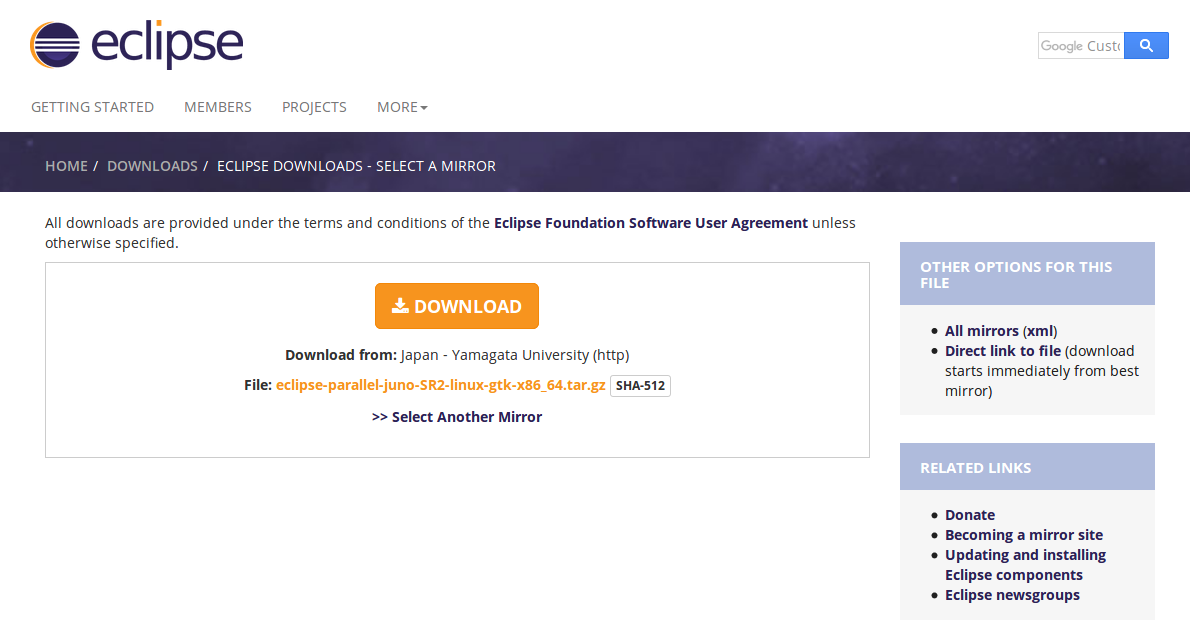
\includegraphics[width=0.8\textwidth]{Figure/AppendixA/eclipse-download-website.png}
	\rule{35em}{0.5pt}
	\caption[Eclipse Oxygen Download Official Website]{Eclipse Oxygen Download Official Website}
\end{figure}

Ensure the Eclipse IDE version selected is compatible with 64-bit Ubuntu Operating System.

\section{GoClipse plugin for Eclipse IDE installation}

\subsection{Eclipse Marketplace}

\begin{figure}[H]
	\centering
	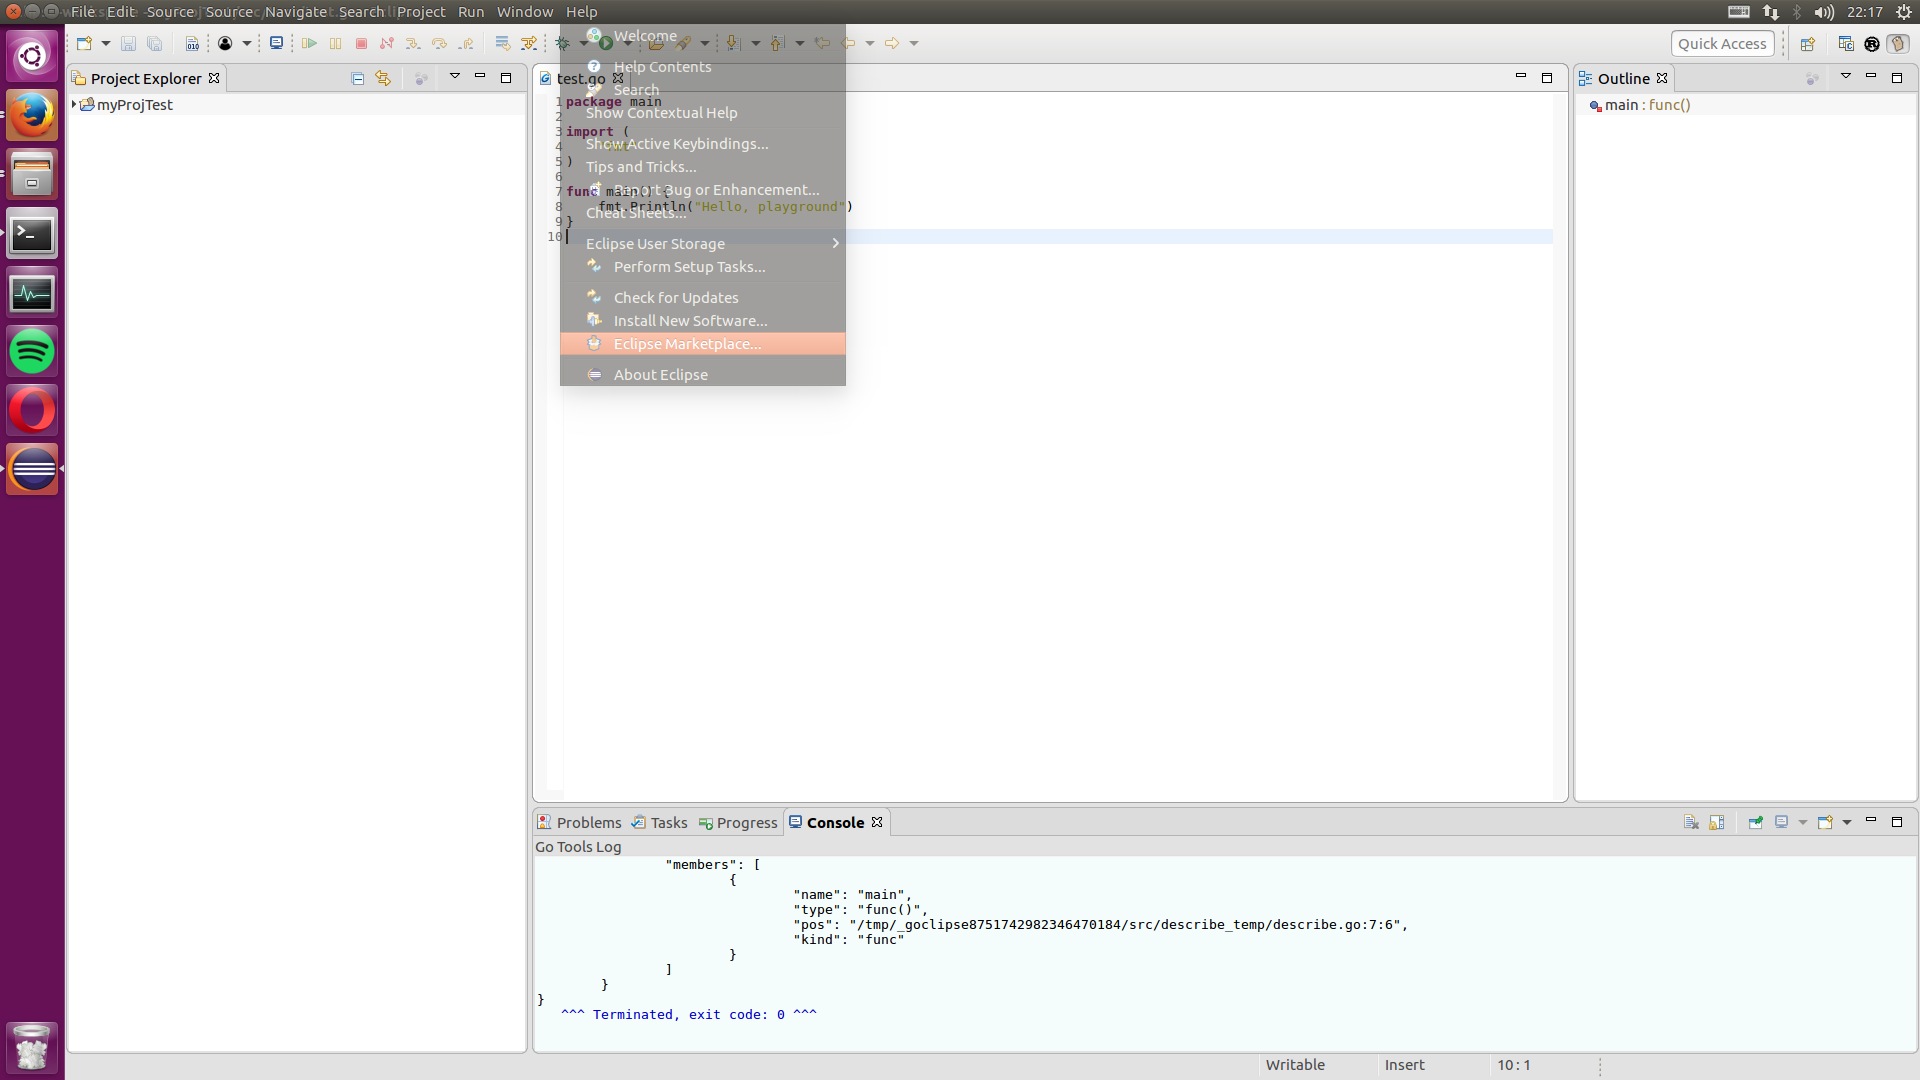
\includegraphics[width=0.8\textwidth]{Figure/AppendixA/goclipse-installation/goclipse-marketplace-1.png}
	\rule{35em}{0.5pt}
	\caption[Eclipse IDE Marketplace]{Eclipse IDE Marketplace}
\end{figure}

Open Eclipse Marketplace from Help and select Eclipse Marketplace to search for GoClipse plugin.

\subsection{Search Marketplace}

\begin{figure}[H]
	\centering
	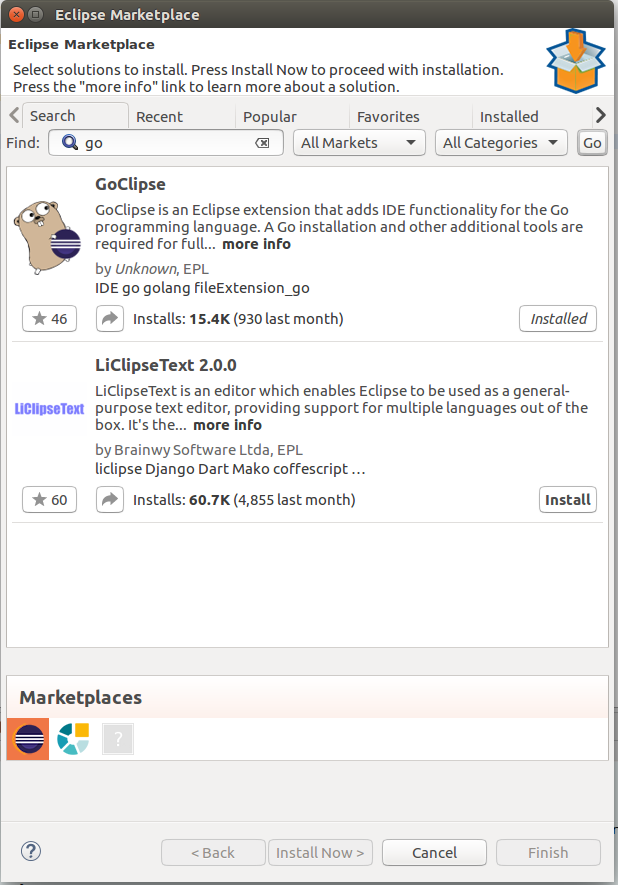
\includegraphics[width=0.3\textwidth]{Figure/AppendixA/goclipse-installation/goclipse-search-marketplace-2.png}
	\rule{35em}{0.5pt}
	\caption[Search Eclipse IDE Marketplace]{Search Eclipse IDE Marketplace}
\end{figure}

Type "Go" in search bar and press Go button to search for available plugin. Press install now to proceed with installation. 

\subsection{Open Perspective}

\begin{figure}[H]
	\centering
	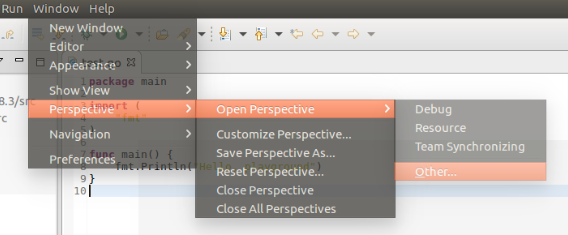
\includegraphics[width=0.5\textwidth]{Figure/AppendixA/goclipse-installation/goclipse-open-perspective-3.png}
	\rule{35em}{0.5pt}
	\caption[Open Perspective]{Open Perspective}
\end{figure}

After the installation is done and success, open Eclipse Perspective by select Window, Perspective, Open Perspective and choose Other.

\subsection{Choose Perspective}

\begin{figure}[H]
	\centering
	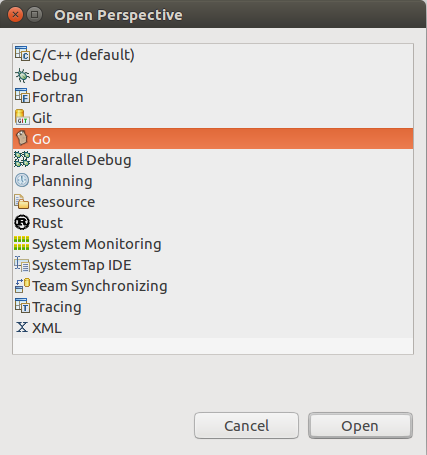
\includegraphics[width=0.8\textwidth]{Figure/AppendixA/goclipse-installation/goclipse-choose-4.png}
	\rule{35em}{0.5pt}
	\caption[Open Perspective]{Choose Go Perspective}
\end{figure}

Choose Go Perspective and press Enter. 

\subsection{Set Go compiler and GOPATH}

\begin{figure}[H]
	\centering
	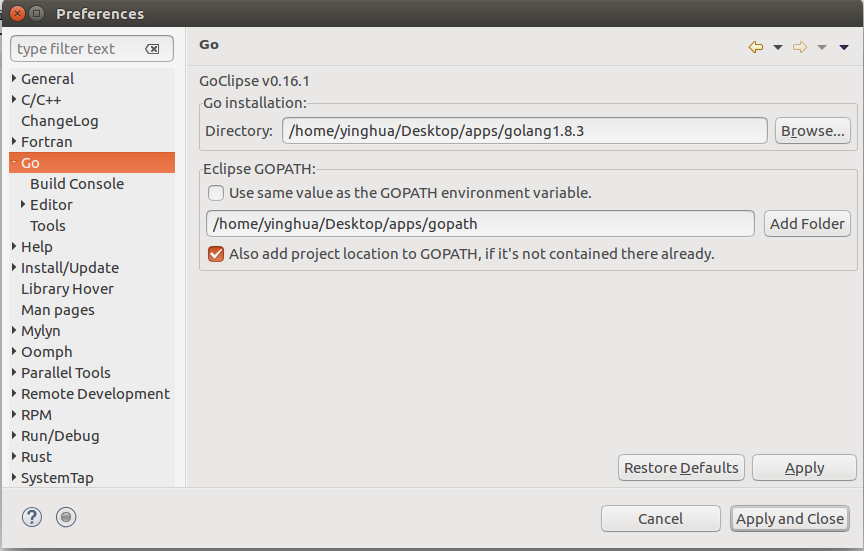
\includegraphics[width=0.8\textwidth]{Figure/AppendixA/goclipse-installation/5- goclipse-setting.png}
	\rule{35em}{0.5pt}
	\caption[Set Go compiler and GOPATH]{Set Go compiler and GOPATH}
\end{figure}

Set Go compiler  and GOPATH into Goclipse plugins. 

\subsection{Set GOCODE, GURU, GODEF and GOFMT path}

\begin{figure}[H]
	\centering
	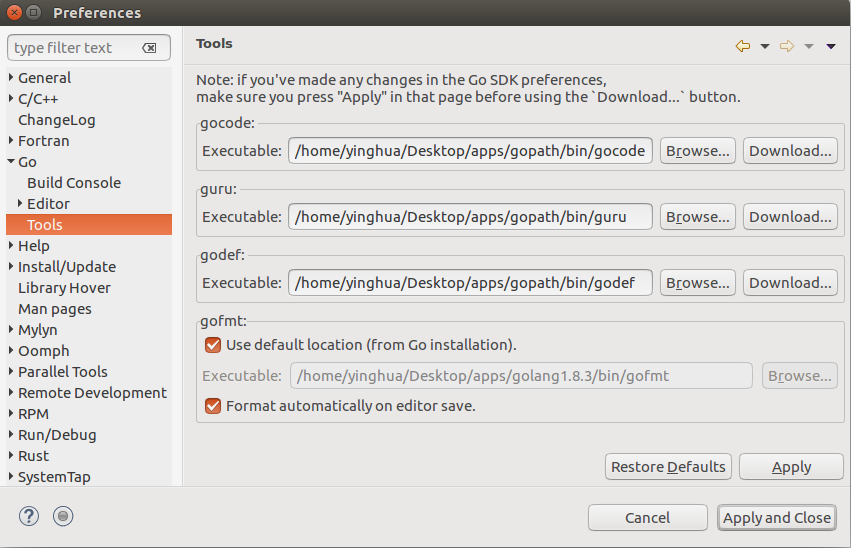
\includegraphics[width=0.8\textwidth]{Figure/AppendixA/goclipse-installation/6-goclipse-setting.png}
	\rule{35em}{0.5pt}
	\caption[Set GOCODE, GURU, GODEF and GOFMT path]{Set GOCODE, GURU, GODEF and GOFMT path}
\end{figure}

Set GOCODE, GURU, GODEF and GOFMT executable path into Goclipse plugins and press "Apply and Close" to complete the setup process. 

\subsection{Test Go compilation in Eclipse IDE}

\begin{figure}[H]
	\centering
	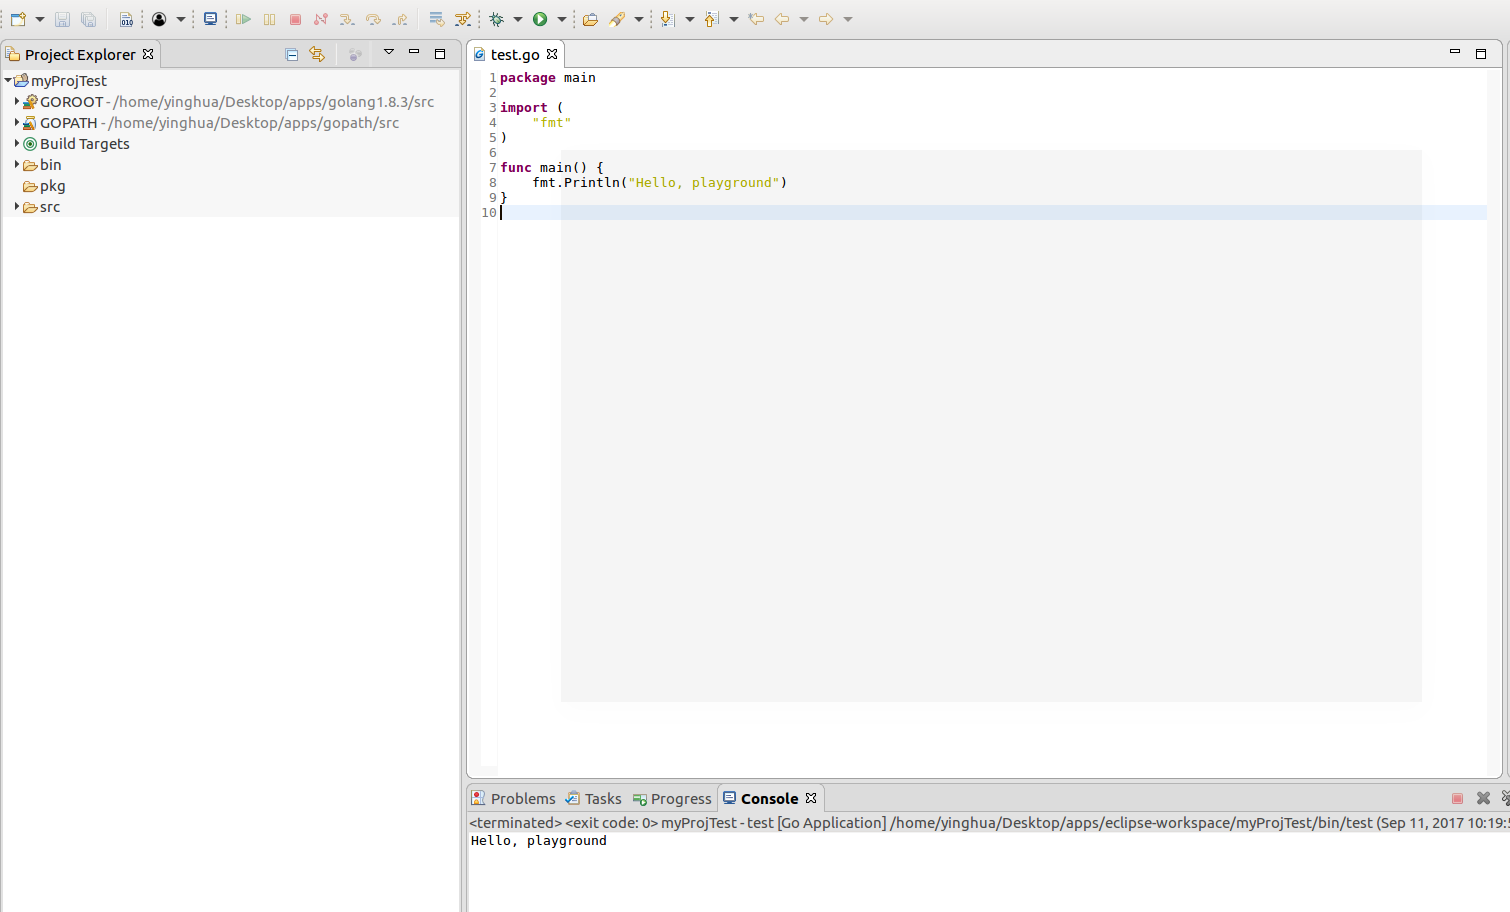
\includegraphics[width=0.8\textwidth]{Figure/AppendixA/goclipse-installation/7-goclipse-success.png}
	\rule{35em}{0.5pt}
	\caption[Test Go compilation in Eclipse IDE]{Test Go compilation in Eclipse IDE}
\end{figure}

Test Go compilation with simple Hello Playground program, the setup process is successful if the Go program is compile and run correctly. 

\section{RustDT plugin for Eclipse IDE installation}

\begin{figure}[H]
	\centering
	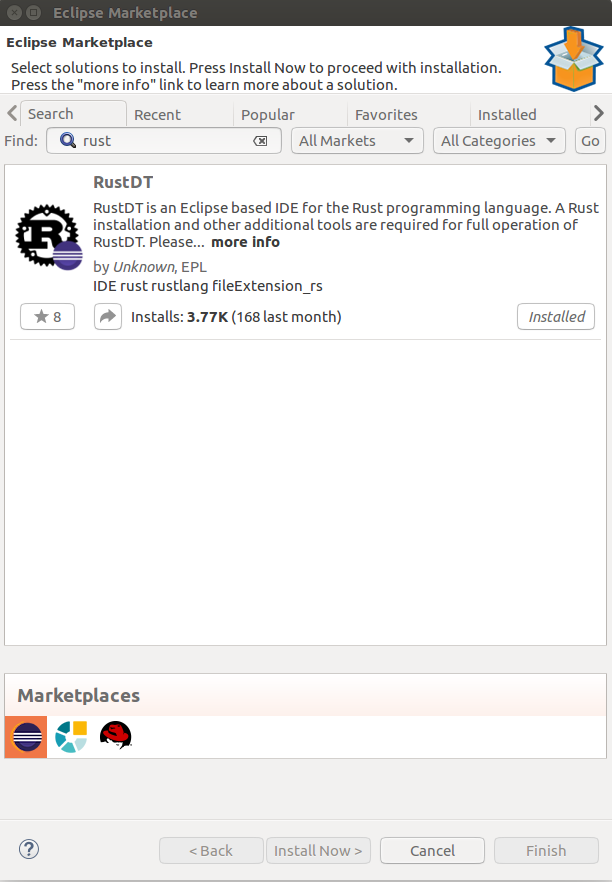
\includegraphics[width=0.6\textwidth]{Figure/AppendixA/rustdt-installation/1-rust-perspective.png}
	\rule{35em}{0.5pt}
	\caption[Test Go compilation in Eclipse IDE]{Test Go compilation in Eclipse IDE}
\end{figure}

Open Eclipse Marketplace similar to step in Appendix A.4.1 to A.4.7. Search the marketplace by type "Rust" in search bar and press Go button to search for tools. Press install now to proceed with installation. The setup process is similar with Goclipse installation process, once the installation and setup is done. The program will compile and run successfully.

\pagebreak  

\section{Linux command for PostgreSQL database installation}

\lstset{basicstyle=\ttfamily\tiny} 
\begin{lstlisting}[breaklines, frame=single, numbers=left, caption={Linux command for PostgreSQL database installation}, label=commandline-02]

===========================================
Step 1 - Install postgreSQL in command line 
===========================================

yinghua@yinghua-NL8C:~$ sudo apt-get update
yinghua@yinghua-NL8C:~$ sudo apt-get install postgresql postgresql-contrib
[sudo] password for yinghua: 

===========================================
Step 2 - Create database for FYP1 
===========================================
postgres=# create database fyp1;
CREATE DATABASE

postgres=# \l
List of databases
Name    |  Owner   | Encoding |   Collate   |    Ctype    |   Access privileges   
-----------+----------+----------+-------------+-------------+-----------------------
fyp1      | postgres | UTF8     | en_US.UTF-8 | en_US.UTF-8 | 
postgres  | postgres | UTF8     | en_US.UTF-8 | en_US.UTF-8 | 
template0 | postgres | UTF8     | en_US.UTF-8 | en_US.UTF-8 | =c/postgres          +
|          |          |             |             | postgres=CTc/postgres
template1 | postgres | UTF8     | en_US.UTF-8 | en_US.UTF-8 | =c/postgres          +
|          |          |             |             | postgres=CTc/postgres
(4 rows)

===========================================
Step 3 - Initial login with postgres user into psql
===========================================
yinghua@yinghua-NL8C:~$ sudo -i -u postgres psql 
psql (9.5.7)
Type "help" for help.

======================================================
Step 4 - Add myself as new user for PostgreSQL with Superuser access
======================================================
yinghua@yinghua-NL8C:~/Documents/FYP/Postcode-data/uk-postcodes-master$ sudo -i -u postgres psql fyp1
[sudo] password for yinghua: 
psql (9.5.7)
Type "help" for help.

postgres@yinghua-NL8C:~$ createuser -P -s -e yinghua
Enter password for new role: 
Enter it again: 
CREATE ROLE yinghua PASSWORD 'md5eec308d944ffa817c37ee6230b0c98eb' SUPERUSER CREATEDB CREATEROLE INHERIT LOGIN;

======================================================
Step 5 - List all the user in PostgreSQL
======================================================
postgres=# \du
List of roles
Role name |                         Attributes                         | Member of 
-----------+------------------------------------------------------------+-----------
postgres  | Superuser, Create role, Create DB, Replication, Bypass RLS | {}
yinghua   | Superuser, Create role, Create DB   


===========================================
Step 6 - Connect FYP1 Database
===========================================
postgres=# \c fyp1
You are now connected to database "fyp1" as user "postgres".

===============================================
Step 7 - Check whether there are tables in FYP1 database
===============================================
fyp1=# \dt
No relations found.

\end{lstlisting}

Install PostgreSQL database with command line using APT package. After the installation is success, create new user for new database in PostgreSQL. 


	
 









\chapter{Data Validation} 
\label{AppendixB} 
\lhead{Appendix B. \emph{Data Validation}} 

% Write your Appendix content below here.
% =========================================

\section{Introduction}
The devil advocation test is conducted to ensure obtained raw CSV data are clean and useful. The test is conduced to ensure:- 

\begin{enumerate}[topsep=0pt,itemsep=-1ex,partopsep=1ex,parsep=1.5ex]
	\item The number of commas in each records should match number of columns in database.
	\item Raw data from CSV should match the column's data type in database for data importation and preparation.
	\item Review and check uniqueness of data in each columns and row.
\end{enumerate}  

\pagebreak

\section{Match number of commas with database columns}

\lstset{basicstyle=\ttfamily\tiny} 
\begin{lstlisting}[breaklines, frame=single, numbers=left, caption={Match number of commas with database columns}, label=commandline-02]

===================
1. connect to database
===================

yinghua@yinghua:~$ psql fyp1;
psql (9.5.8)
Type "help" for help.

==================================
2. create table without one column
==================================

fyp1=# create table subject_test ( ukprn int not null, providername varchar(100) not null, region varchar(100) not null, subject varchar(50) not null, sex varchar(30) not null, yearaftergraduation varchar(30) not null, grads varchar(10) null default null, unmatched varchar(20) null default null, matched varchar(20) null default null, activityNotCaptured varchar(20) default null, nosustdest varchar(20) null default null, sustemponly varchar(20) null default null, sustemp varchar(20) null default null, sustempfsorboth varchar(20) null default null, earningsinclude varchar(20) null default null, lowerannearn varchar(20) null default null, medianannearn varchar(20) null default null, upperannearn varchar(20) null default null, polargrpone varchar(20) null default null, polargrponeincluded varchar(20) null default null, prattband varchar(20) null default null);

========================================================================
3. Terminal return error complains extra data after last expected column
========================================================================

fyp1=# \copy subject_test from 'institution-subject-data.csv' with header csv;

ERROR:  extra data after last expected column

CONTEXT:  COPY subject_test, line 2: "10000291,Anglia Ruskin University,East,Agriculture & related subjects,Female,1,30,x,x,x,x,x,x,x,20,9..."

\end{lstlisting}

In this section, PostgreSQL query is executed on a terminal to check the number of commas match the number of columns possesses in the table. We will purposely remove one column during table creation and try to import all rows of data into PostgreSQL database. 

The terminal will return an error and complains data could not insert into the table because a column is expected during importation process. 
\linebreak

\lstset{basicstyle=\ttfamily\tiny} 
\begin{lstlisting}[breaklines, frame=single, numbers=left, caption={Identify correctness of data types}, label=commandline-02]

========================================================================
4. Add new column into tables and import data successfully
========================================================================

fyp1=# alter table subject_test add column prattincluded varchar(20) null default null;
fyp1=# \copy subject_test from 'institution-subject-data.csv' with header csv;
COPY 32706


\end{lstlisting}

Ultimately, the CSV raw data will import successfully only if the count of commas match the counts of columns in table. 
\pagebreak

\section{Identify correctness and suitability of data types}

\lstset{basicstyle=\ttfamily\tiny} 
\begin{lstlisting}[breaklines, frame=single, numbers=left, caption={Identify correctness of data types}, label=commandline-02]

======================
Step 1. connect to database
======================

yinghua@yinghua:~$ psql fyp1;
psql (9.5.8)
Type "help" for help.

==================================
Step 2. create companydata table
==================================

fyp1=# create table companydata ( CompanyName varchar(160) null default null, CompanyNumber varchar(8) not null primary key, CareOf varchar(100) null, POBOX varchar(10) null, AddressLine1 varchar(300) null, AddressLine2 varchar(300) null, PostTown varchar(50) null, County varchar(50) null, Country varchar(50) null, PostCode varchar(20) null, CompanyCategory varchar(100) not null, CompanyStatus varchar(70) not null, CountryOfOrigin varchar(50) not null, DissolutionDate date null default null, IncorporationDate date null default null, AccountingRefDay int null, AccountingRefMonth int null default 0, Account_NextDueDate date null default null, Account_LastMadeUpdate date null default null, AccountCategory varchar(30) null, Return_NextDueDate date null default null, Return_LastMadeUpDate date null default null, NumMortChanges int null, NumMortOutstanding int null, NumMortPartSatisfied int null, NumMortSatisfied int null, SICCode1 varchar(170) null, SICCode2 varchar(170) null, SICCode3 varchar(170) null, SICCode4 varchar(170) null, NumGenPartners int not null, NumLimPartners int not null, URI varchar(47) not null, pn1_CONDate date null default null, pn1_CompanyName varchar(160) null, pn2_CONDate date null default null, pn2_CompanyName varchar(160) null, pn3_CONDate date null default null, pn3_CompanyName varchar(160) null, pn4_CONDate date null default null, pn4_CompanyName varchar(160) null, pn5_CONDate date null default null, pn5_CompanyName varchar(160) null, pn6_CONDate date null default null, pn6_CompanyName varchar(160) null, pn7_CONDate date null default null, pn7_CompanyName varchar(160) null, pn8_CONDate date null default null, pn8_CompanyName varchar(160) null, pn9_CONDate date null default null, pn9_CompanyName varchar(160) null, pn10_CONDate date null default null, pn10_CompanyName varchar(160) null, ConfStmtNextDueDate date null default null, ConfStmtLastMadeUpDate date null default null);
CREATE TABLE

===========================================
Step 3 - Import data into companydata table
===========================================
fyp1=# \copy companydata from 'Basic-Company-Data-Full.csv' with header csv;

=================================================================================
Step 4 - Terminal return error because double quotes are not allow to insert into date datatypes. 
=================================================================================
ERROR:  invalid input syntax for type date: ""
CONTEXT:  COPY companydata, line 2, column dissolutiondate: ""

\end{lstlisting}

In this section, PostgreSQL query is executed on a terminal to check the suitability and correctness of data types during data importation from CSV files to PostgreSQL database. 

The terminal will return an error and because double quotes are not allow to insert into "date" datatypes. It is caused by the NULL values in company CSV raw data is generated with double quotes and unable to insert them into "date" data types. 

\pagebreak

\lstset{basicstyle=\ttfamily\tiny} 
\begin{lstlisting}[breaklines, frame=single, numbers=left, caption={Remove null values with double quotes in CSV raw data}, label=commandline-02]

=====================================
Step 5 - Remove null value with double quotes for data insertion on DATE DATATYPE
=====================================
yinghua@yinghua-NL8C:~/Documents/FYP/Basic-Company-Data$ sed 's/""//g' Basic-Company-Data-Full.csv > Full.csv

=====================================
Step 6 - Import data into companydata table
=====================================
fyp1=# \copy companydata from 'Full.csv' with header csv;
COPY 4077979

\end{lstlisting}

As the meaning of null values with double quotes and without quotes are the same. To resolve this problem, \textit{seq} command is required produce new files by remove null values with double quotes stores in each columns. The CSV raw data will import successfully if every columns of data match table's column data types. 

\pagebreak

\section{Identify row and column uniqueness in each raw data}

Data redundancy and duplication is an inevitable phenomenon found in million of data obtained from on-line sources. Unintentional duplication of records created from data warehouse are hardly avoided. Therefore, the uniqueness of data has to be check in every row and columns for conduct data de-duplication in Phase 2.
\newline

\subsection{Identify row uniqueness}

\lstset{basicstyle=\ttfamily\tiny} 
\begin{lstlisting}[breaklines, frame=single, numbers=left, caption={Identify row uniqueness}, label=commandline-02]
======================
Step 1. connect to database
======================

yinghua@yinghua:~$ psql fyp1;
psql (9.5.8)
Type "help" for help.

fyp1#Data redundancy and duplication is an inevitable phenomenon found in million of data obtained from on-line sources. Unintentional duplication of records created from the data warehouse 's hard to be avoided. Therefore, the uniqueness of data has to be check in every row and columns for conduct data de-duplication in Phase 2.

======================================================
Step 2 - Verify duplicates row in company data tables
======================================================
fyp1=# select (companydata.*)::text, count(*) from companydata group by companydata.* having count(*) > 1;

 companydata | count 
-------------+-------
(0 rows)

======================================================
Step 3 - Verify duplicates row in subject data tables
======================================================
fyp1=# select (leo.*)::text, count(*) from leo group by leo.* having count(*) > 1; 
  leo    | count 
---------+-------
(0 rows)

======================================================
Step 4 - Verify duplicates row in LEO data tables
======================================================
fyp1=# select (leo.*)::text, count(*) from leo group by leo.* having count(*) > 1; 
  leo    | count 
---------+-------
(0 rows)

======================================================
Step 5: Verify duplicates row in NSPL data table
======================================================
fyp1=# select (nspl.*)::text, count(*) from nspl group by nspl.* having count(*) > 1;
 nspl | count 
------+-------
(0 rows)

\end{lstlisting}

In this section, PostgreSQL query is executed on a terminal to identify duplicates row found in every table. The result shows that there is no row duplication occurs between rows. 

\subsection{Identify column uniqueness}

\lstset{basicstyle=\ttfamily\tiny} 
\begin{lstlisting}[breaklines, frame=single, numbers=left, caption={Identify column uniqueness}, label=commandline-02]
======================
Step 1. connect to database
======================

yinghua@yinghua:~$ psql fyp1;
psql (9.5.8)
Type "help" for help.

===============================
Step 2. List structure of table
===============================

fyp1=# \d+ leo

Table "public.leo"
Column              |          Type          |            Modifiers            | Storage  | 
--------------------+------------------------+---------------------------------+----------+
ukprn               | integer                | not null                        | plain    |
providername        | character varying(100) | not null                        | extended |
region              | character varying(100) | not null                        | extended |
subject             | character varying(50)  | not null                        | extended |
sex                 | character varying(30)  | not null                        | extended |
yearaftergraduation | character varying(30)  | not null                        | extended |
grads               | character varying(10)  | default NULL::character varying | extended |
unmatched           | character varying(20)  | default NULL::character varying | extended |

(more columns are not shown.....)

===============================================================
Step 3. Check duplication of data in selected columns
===============================================================

fyp1=# select ukprn, providername, region, count(*) from leo group by ukprn, providername, region having count(*) > 1;

===============================================================
Step 4. The duplication of columns with rows are return
===============================================================

ukprn   |                    providername                     |          region          | count 
----------+-----------------------------------------------------+--------------------------+-------
10007775 | Queen Mary University of London                     | London                   |   207
10007792 | The University of Exeter                            | South West               |   207
10003324 | The Institute of Cancer Research                    | London                   |   207
10007784 | University College London                           | London                   |   207
10003957 | Liverpool John Moores University                    | North West               |   207
10000886 | The University of Brighton                          | South East               |   207
10007816 | The Royal Central School of Speech and Drama        | London                   |   207
10002681 | Glasgow School of Art                               | Scotland                 |   207
10005545 | Royal Agricultural University                       | South West               |   207
10037449 | University of St Mark and St John                   | South West               |   207
10007144 | The University of East London                       | London                   |   207
10007161 | Teesside University                                 | North East               |   207
10007713 | York St John University                             | Yorkshire and the Humber |   207
10003863 | Leeds Trinity University                            | Yorkshire and the Humber |   207

(more duplication data found in columns are not shown......)


\end{lstlisting}

In this section, PostgreSQL query is executed on a terminal to identify duplicates data found in specific columns. The result shows the count of duplication data found in selected columns and lists out in tabular form. This method is proved to be able to identify data duplication occurs within a column. 





 





\chapter{Golang programming for import CSV into PostgreSQL database} 
\label{AppendixC} 
\lhead{Appendix C. \emph{Golang for import CSV into PostgreSQL database.}} 

% Write your Appendix content below here.
% =========================================

\section{Introduction}

The Go Programming Language possess package csv to reads and write comma-separated values (CSV) files. The package will automatically ignore whitespace, blank lines and delimits commas to read data. In addition, the language also contains a driver to perform CRUD transaction on PostgreSQL database. 

The program below imports 100 rows of company data, LEO data and NSPL data from CSV files to PostgreSQL database. Five columns of data are selected from each file to import into this program as proof of concept in this project. The tables will be created in PostgreSQL database before the program is executed.

\pagebreak

\subsection {LEO table for data importation}

\lstset{basicstyle=\ttfamily\tiny} 
\begin{lstlisting}[breaklines, frame=single, numbers=left, caption={PostgreSQL query for LEO table creation.}, label=commandline-02]

-- File: fyp1-leo.sql
-- Author: Chai Ying Hua 
-- Database: psql (PostgreSQL) 9.5.8

-- ======================================
-- CHANGES IN V1.1(Sun Aug 27. 2017)
-- 	Create leo table for phase 1 to import data
-- ======================================

create table go_subject  ( 
	ukprn int not null, 
	providername varchar(100) not null,
	region varchar(100) not null, 
	subject varchar(50) not null, 
	sex varchar(30) not null
);

\end{lstlisting}

\subsection {NSPL table for data importation}

\lstset{basicstyle=\ttfamily\tiny} 
\begin{lstlisting}[breaklines, frame=single, numbers=left, caption={PostgreSQL query for NSPL table creation.}, label=commandline-02]

-- File: fyp1-nspl.sql
-- Author: Chai Ying Hua 
-- Database: psql (PostgreSQL) 9.5.8

-- ======================================
-- CHANGES IN V1.1(Mon Sep 4. 2017)
-- 	Create nspl table for phase 1 to import data
-- ======================================

create table go_nspl (
	postcode1 varchar(15) not null,
	postcode2 varchar(15) not null primary key,
	date_introduce varchar(10) not null, 
	usertype int not null,
	position_quality int not null
)

\end{lstlisting}

\subsection {LEO table for data importation}

\lstset{basicstyle=\ttfamily\tiny} 
\begin{lstlisting}[breaklines, frame=single, numbers=left, caption={PostgreSQL query for Company table creation.}, label=commandline-02]

-- File: fyp1-company.sql
-- Author: Chai Ying Hua 
-- Database: psql (PostgreSQL) 9.5.8

-- =========================================================================
-- CHANGES IN V1.1(Sun Aug 27. 2017)
-- 	Create companydata table for phase 1 to import data
-- =========================================================================

create table go_company ( 
	CompanyName varchar(160) null default null, 
	CompanyNumber varchar(8) not null primary key,
	CompanyCategory varchar(100) not null,
	CompanyStatus varchar(70) not null
	CountryOfOrigin varchar(50) not null
);

\end{lstlisting}



\subsection{Source code of Go program}

\lstset{basicstyle=\ttfamily\tiny} 
\begin{lstlisting}[breaklines, frame=single, numbers=left, caption={Source code of Go program}, label=commandline-02]

package main

import (
	"bufio"
	"database/sql"
	"encoding/csv"
	"fmt"
	"io"
	"os"
	"strconv"
	
	_ "github.com/lib/pq"
)

const (
	DB_USER                       = "yinghua"
	DB_PASSWORD                   = "123"
	DB_NAME                       = "fyp1"
	COMPANY_FILE_DIRECTORY string = "/home/yinghua/Documents/FYP-data/company-data/company-data-full.csv"
	LEO_FILE_DIRECTORY     string = "/home/yinghua/Documents/FYP-data/subject-data/institution-subject-data.csv"
	NSPL_FILE_DIRECTORY    string = "/home/yinghua/Documents/FYP-data/postcode-data/UK-NSPL.csv"
)

type CompanyData struct {
	name     string
	number   string
	category string
	status   string
	country  string
}

type LEOData struct {
	ukprn   int
	name    string
	region  string
	subject string
	sex     string
}

type NSPLData struct {
	postcode1      string
	postcode2      string
	date_introduce string
	usertype       int
	pos_quality    int
}

var db *sql.DB

//====================================================
//function to check error and print error messages
//====================================================
func checkErr(err error, message string) {
	if err != nil {
		panic(message + " err: " + err.Error())
	}
}

//====================================================
// initialize connection to database
//====================================================
func initDB() {

	dbInfo := fmt.Sprintf("user=%s password=%s dbname=%s sslmode=disable",
	DB_USER, DB_PASSWORD, DB_NAME)
	psqldb, err := sql.Open("postgres", dbInfo)
	checkErr(err, "psql open")
	db = psqldb

}

//====================================================
// Import company data
//====================================================
func importCompanyData() {

	var sStmt string = "insert into go_company values ($1, $2, $3, $4, $5)"
	
	stmt, err := db.Prepare(sStmt)
	checkErr(err, "Prepare Stmt")
	
	// Open CSV files
	csvFile, err := os.Open(COMPANY_FILE_DIRECTORY)
	checkErr(err, "Open CSV")
	
	defer csvFile.Close()
	
	// Create a new reader.
	reader := csv.NewReader(bufio.NewReader(csvFile))
	
	for i := 0; i <= 100; i++ {
		record, err := reader.Read()
		
		// skipped the first line
		if i == 0 {
			continue
		}
		
		// Stop at EOF.
		if err == io.EOF {
			break
		}
		
		company := CompanyData{
			name:     record[0],
			number:   record[1],
			category: record[10],
			status:   record[11],
			country:  record[12],
		}
		
		stmt.Exec(company.name, company.number, company.category, company.status, company.country)
		checkErr(err, "Company Data importation")
	}
}

//====================================================
// Import LEO data
//====================================================
func importSubjectData() {

	var sStmt string = "insert into go_subject values ($1, $2, $3, $4, $5)"
	
	stmt, err := db.Prepare(sStmt)
	checkErr(err, "Prepare Subject Stmt")
	
	csvFile, err := os.Open(LEO_FILE_DIRECTORY)
	checkErr(err, "Open LEO CSV")
	
	defer csvFile.Close()
	
	// Create a new reader.
	reader := csv.NewReader(bufio.NewReader(csvFile))
	
	for i := 0; i <= 100; i++ {
		record, err := reader.Read()
		
		// skipped the first line
		if i == 0 {
			continue
		}
		
		// Stop at EOF.
		if err == io.EOF {
			break
		}
		
		integer, err := strconv.Atoi(record[0])
		checkErr(err, "Convert UKRPN to Integer")
		
		subject := LEOData{
			ukprn:   integer,
			name:    record[1],
			region:  record[2],
			subject: record[3],
			sex:     record[4],
		}
		
			stmt.Exec(subject.ukprn, subject.name, subject.region, subject.subject, subject.sex)
			checkErr(err, "Subject Data importation")
		}
}

//====================================================
// Import NSPL data
//====================================================
func importNSPLData() {

	var sStmt string = "insert into go_nspl values ($1, $2, $3, $4, $5)"
	
	stmt, err := db.Prepare(sStmt)
	checkErr(err, "Prepare Postcode Stmt")
	
	csvFile, err := os.Open(NSPL_FILE_DIRECTORY)
	checkErr(err, "Open Postcode CSV")
	
	defer csvFile.Close()
	
	// Create a new reader.
	reader := csv.NewReader(bufio.NewReader(csvFile))

	for i := 0; i <= 100; i++ {
		record, err := reader.Read()
		
		// skipped the first line
		if i == 0 {
		continue
		}
		
		// Stop at EOF.
		if err == io.EOF {
		break
		}
		
		userInt, err := strconv.Atoi(record[4])
		checkErr(err, "Convert Usertype to Integer")
		
		posInt, err := strconv.Atoi(record[7])
		checkErr(err, "Convert Usertype to Integer")
	
		postcode := NSPLData {
		postcode1:      record[0],
		postcode2:      record[1],
		date_introduce: record[3],
		usertype:       userInt,
		pos_quality:    posInt,
		}
	
		stmt.Exec(postcode.postcode1, postcode.postcode2, postcode.date_introduce, postcode.usertype, postcode.pos_quality)
		checkErr(err, "Postcode Data importation")
	}
}

func main() {

	initDB()
	importCompanyData()
	importSubjectData()
	importNSPLData()

}

/**

yinghua@yinghua:~/Desktop/apps/eclipse-workspace/FYP1/src/postgres-process$ go build import-csv-psql.go
yinghua@yinghua:~/Desktop/apps/eclipse-workspace/FYP1/src/postgres-process$ time go run import-csv-psql.go

real	0m3.647s
user	0m0.328s
sys	0m0.096s
yinghua@yinghua:~/Desktop/apps/eclipse-workspace/FYP1/src/postgres-process$

**/

\end{lstlisting}

\chapter{Sequential and concurrent programming with Golang on PostgreSQL database retrieval.} 
\label{AppendixD} 
\lhead{Appendix D. \emph{Sequential and concurrent programming with Golang on PostgreSQL database retrieval.}}

% Write your Appendix content below here.
% =========================================

\section {Golang Sequential Program Source Code}

\lstset{basicstyle=\ttfamily\tiny}  
\begin{lstlisting}[breaklines, frame=single, numbers=left, caption={Golang Sequential Program Source Code}, label=commandline-02]

package main

	import (
	"database/sql"
	"fmt"
	"time"
	
	_ "github.com/lib/pq"
)

const (
	DB_USER     = "yinghua"
	DB_PASSWORD = "123"
	DB_NAME     = "fyp1"
)

var db *sql.DB

//====================================================
//function to check error and print error messages
//====================================================
func checkErr(err error, message string) {
	if err != nil {
		panic(message + " err: " + err.Error())
	}
}

//====================================================
// initialize connection with database
//====================================================
func initDB() {

	dbInfo := fmt.Sprintf("user=%s password=%s dbname=%s sslmode=disable",
	DB_USER, DB_PASSWORD, DB_NAME)
	psqldb, err := sql.Open("postgres", dbInfo)
	checkErr(err, "Initialize database")
	db = psqldb

}

//====================================================
// retrieve data from company table in postgres
//====================================================
func retrieveCompanyData() {

	fmt.Println("Start retrieve company data from database ... ")
	start := time.Now()
	
	time.Sleep(time.Second * 2)
	
	rows, err := db.Query("SELECT c.companyname, c.companynumber, c.companycategory, c.companystatus, c.countryoforigin FROM companydata AS c ORDER BY c.companynumber limit 100;")
	checkErr(err, "Query Company DB rows")
	
	var (
		companyname     string
		companynumber   string
		companycategory string
		companystatus   string
		countryoforigin string
	)
	
	for rows.Next() {
		err = rows.Scan(&companyname, &companynumber, &companycategory, &companystatus, &countryoforigin)
		checkErr(err, "Read company data rows")
		//fmt.Printf("%8v %3v %6v %6v %6v\n", companyname, companynumber, companycategory, companystatus, countryoforigin)
	}
	
	fmt.Println("Data retrieval of company data SUCCESS! ")
	fmt.Printf("%.8fs elapsed\n\n", time.Since(start).Seconds())

}

//====================================================
// retrieve data from postcode table in postgres
//====================================================
func retrievePostcodeData() {

	fmt.Println("Start retrieve postcode data from database ... ")
	start := time.Now()
	
	time.Sleep(time.Second * 2)
	
	rows, err := db.Query("SELECT postcode1, postcode2, date_introduce, usertype, position_quality FROM go_nspl LIMIT 50")
	checkErr(err, "Query Postcode DB rows")
	
	var (
		postcode1        string
		postcode2        string
		date_introduce   string
		usertype         int
		position_quality int
	)
	
	for rows.Next() {
		err = rows.Scan(&postcode1, &postcode2, &date_introduce, &usertype, &position_quality)
		checkErr(err, "Read postcode data rows")
		//fmt.Printf("%6v %8v %6v %6v %6v\n", postcode1, postcode2, date_introduce, usertype, position_quality)
	}
	
	fmt.Print("Data retrieval of postcode data SUCCESS! ")
	fmt.Printf("%.8fs elapsed\n\n", time.Since(start).Seconds())

}

//====================================================
// retrieve data from subject table in postgres
//====================================================
func retrieveSubjectData() {

	fmt.Println("Start retrieve LEO data from database ... ")
	start := time.Now()
	
	time.Sleep(time.Second * 2)
	
	rows, err := db.Query("SELECT ukprn, providername, region, subject, sex FROM go_subject LIMIT 50")
	checkErr(err, "Query subject DB rows")
	
	var (
		ukprn   int
		name    string
		region  string
		subject string
		sex     string
	)
	
	for rows.Next() {
		err = rows.Scan(&ukprn, &name, &region, &subject, &sex)
		checkErr(err, "Read subject data rows")
		//fmt.Printf("%6v %8v %6v %6v %6v\n", ukprn, name, region, subject, sex)
	}
	
	fmt.Print("Data retrieval of subject data SUCCESS! ")
	fmt.Printf(" %.8fs elapsed\n\n", time.Since(start).Seconds())

}

//====================================================
// Main function
//====================================================
func main() {

	// get the time before execution
	start := time.Now()
	
	initDB()
	retrieveCompanyData()
	retrievePostcodeData()
	retrieveSubjectData()
	
	// print the time after execution
	fmt.Printf("Total execution %.5fs elapsed\n", time.Since(start).Seconds())

}

/**

yinghua@yinghua:~/Desktop/apps/eclipse-workspace/FYP1/src/postgres-process$ go build sequential-psql.go
yinghua@yinghua:~/Desktop/apps/eclipse-workspace/FYP1/src/postgres-process$ time go run sequential-psql.go
Start retrieve company data from database ...
Data retrieval of company data SUCCESS!
2.00721985s elapsed

Start retrieve postcode data from database ...
Data retrieval of postcode data SUCCESS!
2.00144933s elapsed

Start retrieve LEO data from database ...
Data retrieval of subject data SUCCESS!
2.00131415s elapsed

Total execution 6.01005s elapsed

real	0m6.252s
user	0m0.272s
sys		0m0.032s


**/


\end{lstlisting}

\pagebreak

\subsection {Golang Concurrent Program Source Code}

\lstset{basicstyle=\ttfamily\tiny} 
\begin{lstlisting}[breaklines, frame=single, numbers=left, caption={Golang Concurrent Program Source Code}, label=commandline-02]

package main

import (
	"database/sql"
	"fmt"
	"time"
	
	_ "github.com/lib/pq"
)

//====================================================
// database information
//====================================================
const (
	DB_USER     = "yinghua"
	DB_PASSWORD = "123"
	DB_NAME     = "fyp1"
)

var (
	db          *sql.DB
	numChannels int = 3
)

//====================================================
// function to check error and print error messages
//====================================================
func checkErr(err error, message string) {
	if err != nil {
		panic(message + " err: " + err.Error())
	}
}

//====================================================
// initialize connection with database
//====================================================
func initDB() {

	dbInfo := fmt.Sprintf("user=%s password=%s dbname=%s sslmode=disable",
	DB_USER, DB_PASSWORD, DB_NAME)
	psqldb, err := sql.Open("postgres", dbInfo)
	checkErr(err, "Initialize database")
	db = psqldb

}

//====================================================
// retrieve company data store in postgres database
//====================================================
func retrieveCompanyData(ch_company chan string) {

	fmt.Println("Start retrieve company data from database ... ")
	start := time.Now()
	
	time.Sleep(time.Second * 2)
	
	rows, err := db.Query("SELECT c.companyname, c.companynumber, c.companycategory, c.companystatus, c.countryoforigin FROM companydata AS c ORDER BY c.companynumber limit 100;")
	checkErr(err, "Query Company DB rows")
	
	var (
		companyname     string
		companynumber   string
		companycategory string
		companystatus   string
		countryoforigin string
	)
	
	for rows.Next() {
		err = rows.Scan(&companyname, &companynumber, &companycategory, &companystatus, &countryoforigin)
		checkErr(err, "Read company data rows")
		//fmt.Printf("%8v %3v %6v %6v %6v\n", companyname, companynumber, companycategory, companystatus, countryoforigin)
	}
	
	fmt.Printf("%.8fs elapsed\n", time.Since(start).Seconds())
	ch_company <- "Retrieval of company data success. \n"
}

//====================================================
// retrieve postcode data store in postgres database
//====================================================
func retrievePostcodeData(ch_postcode chan string) {
	
	fmt.Println("Start retrieve postcode data from database ... ")
	start := time.Now()
	
	time.Sleep(time.Second * 2)
	
	rows, err := db.Query("SELECT postcode1, postcode2, date_introduce, usertype, position_quality FROM go_nspl LIMIT 50")
	checkErr(err, "Query Postcode DB rows")
	
	var (
		postcode1        string
		postcode2        string
		date_introduce   string
		usertype         int
		position_quality int
	)
	
	for rows.Next() {
		err = rows.Scan(&postcode1, &postcode2, &date_introduce, &usertype, &position_quality)
		checkErr(err, "Read postcode data rows")
		//fmt.Printf("%6v %8v %6v %6v %6v\n", postcode1, postcode2, date_introduce, usertype, position_quality)
	}
	
	fmt.Printf("%.8fs elapsed\n", time.Since(start).Seconds())
		ch_postcode <- "Retrieval of postcode success. \n"
	}
	
	//====================================================
	// retrieve subject data store in postgres database
	//====================================================
	func retrieveSubjectData(ch_subject chan string) {
	
		fmt.Println("Start retrieve LEO data from database ... ")
		start := time.Now()
		
		time.Sleep(time.Second * 2)
		
		rows, err := db.Query("SELECT ukprn, providername, region, subject, sex FROM go_subject LIMIT 50")
		checkErr(err, "Query subject DB rows")
		
		var (
			ukprn   int
			name    string
			region  string
			subject string
			sex     string
		)
		
		for rows.Next() {
			err = rows.Scan(&ukprn, &name, &region, &subject, &sex)
			checkErr(err, "Read subject data rows")
			//fmt.Printf("%6v %8v %6v %6v %6v\n", ukprn, name, region, subject, sex)
		}
		
		fmt.Printf("%.8fs elapsed\n", time.Since(start).Seconds())
			ch_subject <- "Retrieval of subject data success. \n"
		}
		
		// select function
		func goSelect(ch_company, ch_subject, ch_postcode chan string) {
		
		for i := 0; i < numChannels; i++ {
		
			select {
			case msg1 := <-ch_postcode:
				fmt.Println(msg1)
			case msg2 := <-ch_company:
				fmt.Println(msg2)
			case msg3 := <-ch_subject:
				fmt.Println(msg3)
		
		}
	
	}
}

//====================================================
// Main function
//====================================================
func main() {
	
	// make three channel for three functions
	ch_company := make(chan string)
	ch_subject := make(chan string)
	ch_postcode := make(chan string)
	
	// get the time before execution
	start := time.Now()
	
	initDB()
	
	//go routines
	go retrieveCompanyData(ch_company)
	go retrieveSubjectData(ch_subject)
	go retrievePostcodeData(ch_postcode)
	
	goSelect(ch_company, ch_subject, ch_postcode)
	
	// obtain the time after execution
	fmt.Printf("Total execution %.5fs elapsed\n", time.Since(start).Seconds())

}

/**

yinghua@yinghua:~/Desktop/apps/eclipse-workspace/FYP1/src/postgres-process$ go build concurrent-psql.go
yinghua@yinghua:~/Desktop/apps/eclipse-workspace/FYP1/src/postgres-process$ time go run concurrent-psql.go
Start retrieve postcode data from database ...
Start retrieve company data from database ...
Start retrieve LEO data from database ...
2.00615007s elapsed
Retrieval of subject data success.

2.00661550s elapsed
Retrieval of postcode success.

2.00745319s elapsed
Retrieval of company data success.

Total execution 2.00754s elapsed

real	0m2.268s
user	0m0.244s
sys		0m0.076s



**/

)

\end{lstlisting}


\chapter{Sequential and concurrent programming with Golang on reading CSV file} 
\label{AppendixD} 
\lhead{Appendix D. \emph{Sequential and concurrent programming with Golang on PostgreSQL database retrieval.}}

% Write your Appendix content below here.
% =========================================

\section {Golang Sequential Program Source Code}

\lstset{basicstyle=\ttfamily\tiny}  
\begin{lstlisting}[breaklines, frame=single, numbers=left, caption={Golang Sequential Program Source Code}, label=commandline-02]

package main

import (
	"bufio"
	"database/sql"
	"encoding/csv"
	"fmt"
	"io"
	"os"
	"time"
	
	_ "github.com/lib/pq"
)

const (
	DB_USER                       = "yinghua"
	DB_PASSWORD                   = "123"
	DB_NAME                       = "fyp1"
	COMPANY_FILE_DIRECTORY string = "/home/yinghua/Documents/FYP-data/company-data/company-data-full.csv"
	LEO_FILE_DIRECTORY     string = "/home/yinghua/Documents/FYP-data/subject-data/institution-subject-data.csv"
	NSPL_FILE_DIRECTORY    string = "/home/yinghua/Documents/FYP-data/postcode-data/UK-NSPL.csv"
)

var db *sql.DB

// function to check error and print error messages
func checkErr(err error, message string) {
	if err != nil {
		panic(message + " err: " + err.Error())
	}
}

func read_CompanyCSV() {
	
	fmt.Println("Start reading 100 row Company CSV data")
	
	time.Sleep(time.Second * 2)
	
	csvFile, err := os.Open(COMPANY_FILE_DIRECTORY)
	checkErr(err, "Open CSV")
	
	defer csvFile.Close()
	
	// Create a new reader.
	reader := csv.NewReader(bufio.NewReader(csvFile))
	
	for i := 0; i <= 100; i++ {
		_, err := reader.Read()
		
		// skipped the first line
		if i == 0 {
			continue
		}
		
		// Stop at EOF.
		if err == io.EOF {
			break
		}
	
	}
	
	fmt.Println("Finish reading Company CSV data")

}

func read_LEOCSV() {

	fmt.Println("Start reading 100 row LEO CSV data")
	
	time.Sleep(time.Second * 2)
	
	csvFile, err := os.Open(LEO_FILE_DIRECTORY)
	checkErr(err, "Open LEO CSV")
	
	defer csvFile.Close()
	
	// Create a new reader.
	reader := csv.NewReader(bufio.NewReader(csvFile))
	
	for i := 0; i <= 100; i++ {
		_, err := reader.Read()
		
		// skipped the first line
		if i == 0 {
			continue
		}
		
		// Stop at EOF.
		if err == io.EOF {
			break
		}
	}
	
	fmt.Println("Finish readying LEO CSV data")

}

func read_NSPLCSV() {

	fmt.Println("Start reading 100 row NSPL CSV data")
	
	time.Sleep(time.Second * 2)
	
	csvFile, err := os.Open(NSPL_FILE_DIRECTORY)
	checkErr(err, "Open Postcode CSV")
	
	defer csvFile.Close()
	
	// Create a new reader.
	reader := csv.NewReader(bufio.NewReader(csvFile))
	
	for i := 0; i <= 100; i++ {
		_, err := reader.Read()
	
	// skipped the first line
		if i == 0 {
			continue
		}
	
	// Stop at EOF.
		if err == io.EOF {
			break
		}
	}
	
	fmt.Println("Finish readying LEO CSV data")

}

func main() {

	// get the time before execution
	start := time.Now()
	
	read_CompanyCSV()
	read_LEOCSV()
	read_NSPLCSV()
	
	// obtain the time after execution
	fmt.Printf("Total execution %.5fs elapsed\n", time.Since(start).Seconds())

}

/**

yinghua@yinghua:~/Desktop/apps/eclipse-workspace/FYP1/src/postgres-process$ go build sequential-read-csv.go
yinghua@yinghua:~/Desktop/apps/eclipse-workspace/FYP1/src/postgres-process$ time go run sequential-read-csv.go
Start reading 100 row Company CSV data
Finish reading Company CSV data
Start reading 100 row LEO CSV data
Finish readying LEO CSV data
Start reading 100 row NSPL CSV data
Finish readying LEO CSV data
Total execution 6.00823s elapsed

real	0m6.285s
user	0m0.316s
sys		0m0.056s
**/



\end{lstlisting}

\subsection {Golang Concurrent Program Source Code}

\lstset{basicstyle=\ttfamily\tiny} 
\begin{lstlisting}[breaklines, frame=single, numbers=left, caption={Golang Concurrent Program Source Code}, label=commandline-02]

package main

import (
	"bufio"
	"database/sql"
	"encoding/csv"
	"fmt"
	"io"
	"os"
	"time"
	
	_ "github.com/lib/pq"
)

const (
	DB_USER                       = "yinghua"
	DB_PASSWORD                   = "123"
	DB_NAME                       = "fyp1"
	COMPANY_FILE_DIRECTORY string = "/home/yinghua/Documents/FYP-data/company-data/company-data-full.csv"
	LEO_FILE_DIRECTORY     string = "/home/yinghua/Documents/FYP-data/subject-data/institution-subject-data.csv"
	NSPL_FILE_DIRECTORY    string = "/home/yinghua/Documents/FYP-data/postcode-data/UK-NSPL.csv"
)

var (
	db          *sql.DB
	numChannels int = 3
)

// function to check error and print error messages
func checkErr(err error, message string) {
	if err != nil {
		panic(message + " err: " + err.Error())
	}
}

func read_CompanyCSV(ch_company chan string) {

	fmt.Println("Start reading 100 row Company CSV data")
	
	time.Sleep(time.Second * 2)
	
	csvFile, err := os.Open(COMPANY_FILE_DIRECTORY)
	checkErr(err, "Open CSV")
	
	defer csvFile.Close()
	
	// Create a new reader.
	reader := csv.NewReader(bufio.NewReader(csvFile))
	
	for i := 0; i <= 100; i++ {
		_, err := reader.Read()
		
		// skipped the first line
		if i == 0 {
			continue
		}
		
		// Stop at EOF.
		if err == io.EOF {
			break
		}
	}
	
	ch_company <- "Finish readying LEO CSV data"

}

func read_LEOCSV(ch_leo chan string) {

	fmt.Println("Start reading 100 row LEO CSV data")
	
	time.Sleep(time.Second * 2)
	
	csvFile, err := os.Open(LEO_FILE_DIRECTORY)
	checkErr(err, "Open LEO CSV")
	
	defer csvFile.Close()
	
	// Create a new reader.
	reader := csv.NewReader(bufio.NewReader(csvFile))
	
	for i := 0; i <= 100; i++ {
		_, err := reader.Read()
	
		// skipped the first line
		if i == 0 {
			continue
		}
		
		// Stop at EOF.
		if err == io.EOF {
			break
		}
	}

	ch_leo <- "Finish reading LEO CSV data"

}

func read_NSPLCSV(ch_nspl chan string) {

	fmt.Println("Start reading 100 row NSPL CSV data")
	
	time.Sleep(time.Second * 2)
	
	csvFile, err := os.Open(NSPL_FILE_DIRECTORY)
	checkErr(err, "Open Postcode CSV")
	
	defer csvFile.Close()
	
	// Create a new reader.
	reader := csv.NewReader(bufio.NewReader(csvFile))
	
	for i := 0; i <= 100; i++ {
		_, err := reader.Read()
		
		// skipped the first line
		if i == 0 {
			continue
		}
		
		// Stop at EOF.
		if err == io.EOF {
			break
		}
	}
	
	ch_nspl <- "Finish reading NSPL CSV data"
}

// select function
func goSelect(ch_company, ch_leo, ch_nspl chan string) {

	for i := 0; i < numChannels; i++ {
	
		select {
			case msg1 := <-ch_leo:
				fmt.Println(msg1)
			case msg2 := <-ch_company:
			fmt.Println(msg2)
				case msg3 := <-ch_nspl:
			fmt.Println(msg3)
			
		}
		
	}
}

func main() {

	// make three channel for three functions
	ch_company := make(chan string)
	ch_leo := make(chan string)
	ch_nspl := make(chan string)
	
	// get the time before execution
	start := time.Now()
	
	go read_CompanyCSV(ch_company)
	go read_LEOCSV(ch_leo)
	go read_NSPLCSV(ch_nspl)
	
	goSelect(ch_company, ch_leo, ch_nspl)
	
	// obtain the time after execution
	fmt.Printf("Total execution %.5fs elapsed\n", time.Since(start).Seconds())

}

/**

yinghua@yinghua:~/Desktop/apps/eclipse-workspace/FYP1/src/postgres-process$ go build concurrent-read-csv.go
yinghua@yinghua:~/Desktop/apps/eclipse-workspace/FYP1/src/postgres-process$ time go run concurrent-read-csv.go
Start reading 100 row NSPL CSV data
Start reading 100 row Company CSV data
Start reading 100 row LEO CSV data
Finish reading LEO CSV data
Finish reading NSPL CSV data
Finish readying LEO CSV data
Total execution 2.00376s elapsed

real	0m2.243s
user	0m0.264s
sys		0m0.044s

**/


\end{lstlisting}


\chapter{Result of Sequential and concurrent programming with Golang on process CSV} 
\label{AppendixF} 
\lhead{Appendix F. \emph{Result of Golang on process CSV}}

% Write your Appendix content below here.
% =========================================

\section {Linux command for Go program execution}

\lstset{basicstyle=\ttfamily\tiny}  
\begin{lstlisting}[breaklines, frame=single, numbers=left, caption={Linux command for Go program execution}, label=commandline-02]
================================================================
Step 1 - Build sequential-read-csv.go 
================================================================
yinghua@yinghua:~/Desktop/apps/eclipse-workspace/FYP1/src/postgres-process$ go build sequential-read-csv.go

================================================================
Step 2 - Execute sequential-read-csv.go program
================================================================
yinghua@yinghua:~/Desktop/apps/eclipse-workspace/FYP1/src/postgres-process$ time go run sequential-read-csv.go
Start reading 100 row Company CSV data
Finish reading Company CSV data
Start reading 100 row LEO CSV data
Finish readying LEO CSV data
Start reading 100 row NSPL CSV data
Finish readying LEO CSV data
Total execution 6.00823s elapsed

real	0m6.285s
user	0m0.316s
sys	0m0.056s

================================================================
Step 3 - Build concurrent-read-csv.go 
================================================================
yinghua@yinghua:~/Desktop/apps/eclipse-workspace/FYP1/src/postgres-process$ go build concurrent-read-csv.go

================================================================
Step 4 - Execute concurrent-read-csv.go program 
================================================================
yinghua@yinghua:~/Desktop/apps/eclipse-workspace/FYP1/src/postgres-process$ time go run concurrent-read-csv.go
Start reading 100 row NSPL CSV data
Start reading 100 row Company CSV data
Start reading 100 row LEO CSV data
Finish reading LEO CSV data
Finish reading NSPL CSV data
Finish readying LEO CSV data
Total execution 2.00376s elapsed

real	0m2.243s
user	0m0.264s
sys	0m0.044s
\end{lstlisting}

\section{Result of Golang programming on process CSV}

\begin{table}[H]
	\centering
	\begin{tabulary}{1.0\textwidth}{|L|L|L|L}
		\hline
		{\bf Elapsed Time} & {\bf sequential-read-csv.go}  & {\bf concurrent-read-csv.go} \\ \hline
		real      & 6.285s                    &  2.243s                  \\ \hline
		user     & 0.316s                    &  0.264s                  \\ \hline
		sys       & 0.056s                    &  0.044s                  \\ \hline
	\end{tabulary}
	\caption{Result of Golang programming on process CSV raw data}
\end{table}







\chapter{Result of Sequential and concurrent programming with Golang on process PostgreSQL database.} 
\label{AppendixG} 
\lhead{Appendix G. \emph{Result of Golang on process PostgreSQL database}}

% Write your Appendix content below here.
% =========================================

\section {Linux command for Go program execution}

\lstset{basicstyle=\ttfamily\tiny}  
\begin{lstlisting}[breaklines, frame=single, numbers=left, caption={Linux command for Go program execution}, label=commandline-02]

================================================================
Step 1 - Build sequential-psql.go 
================================================================
yinghua@yinghua:~/Desktop/apps/eclipse-workspace/FYP1/src/postgres-process$ go build sequential-psql.go

================================================================
Step 2 - Execute sequential-psql.go program
================================================================
yinghua@yinghua:~/Desktop/apps/eclipse-workspace/FYP1/src/postgres-process$ time go run sequential-psql.go
Start retrieve company data from database ...
Data retrieval of company data SUCCESS!
2.00721985s elapsed

Start retrieve postcode data from database ...
Data retrieval of postcode data SUCCESS!
2.00144933s elapsed

Start retrieve LEO data from database ...
Data retrieval of subject data SUCCESS!
2.00131415s elapsed

Total execution 6.01005s elapsed

real	0m6.252s
user	0m0.272s
sys	0m0.032s

================================================================
Step 3 - Build concurrent-psql.go
================================================================
yinghua@yinghua:~/Desktop/apps/eclipse-workspace/FYP1/src/postgres-process$ go build concurrent-psql.go

================================================================
Step 4 - Execute concurrent-psql.go program 
================================================================
yinghua@yinghua:~/Desktop/apps/eclipse-workspace/FYP1/src/postgres-process$ time go run concurrent-psql.go
Start retrieve postcode data from database ...
Start retrieve company data from database ...
Start retrieve LEO data from database ...
2.00615007s elapsed
Retrieval of subject data success.

2.00661550s elapsed
Retrieval of postcode success.

2.00745319s elapsed
Retrieval of company data success.

Total execution 2.00754s elapsed

real	0m2.268s
user	0m0.244s
sys	0m0.076s



\end{lstlisting}

\section{Result of Golang programming on process PostgreSQL database}

\begin{table}[H]
	\centering
	\begin{tabulary}{1.0\textwidth}{|L|L|L|L}
		\hline
		{\bf Elapsed Time} & {\bf sequential-psql.go}  & {\bf concurrent-psql.go} \\ \hline
		real      & 6.252s                    &  2.268s                  \\ \hline
		user     & 0.272s                    &  0.244s                  \\ \hline
		sys       & 0.032s                    &  0.076s                  \\ \hline
	\end{tabulary}
	\caption{Result of Golang programming on PostgreSQL database}
\end{table}






\chapter{Result of import data from CSV file to PostgreSQL database with Golang} 
\label{AppendixH} 
\lhead{Appendix H. \emph{Result of import data from CSV file to PostgreSQL database with Golang.}}

% Write your Appendix content below here.
% =========================================

\section {Linux command for import data}

\lstset{basicstyle=\ttfamily\tiny}  
\begin{lstlisting}[breaklines, frame=single, numbers=left, caption={Linux command for import data}, label=commandline-02]
=====================================
Step 1 - Connect to FYP1 database
=====================================

yinghua@yinghua:~/Desktop/apps/eclipse-workspace/FYP1/src/postgres-process$ psql fyp1;
psql (9.5.8)
Type "help" for help.

fyp1=#

=====================================
Step 2 - Check number of tables
=====================================
fyp1=# \d
List of relations
Schema |    Name     | Type  |  Owner  
--------+-------------+-------+---------
public | companydata | table | yinghua
public | leo         | table | yinghua
public | nspl        | table | yinghua
(3 rows)

==================================================================
Step 3 - Create go_company table ready for importation 
==================================================================

fyp1=# create table go_company (companyname varchar(160) null default null, companynumber varchar(8) not null primary key, companycategory varchar(100) not null, companystatus varchar(70) not null, countryoforigin varchar(50) not null );
CREATE TABLE

==================================================================
Step 4 - Create go_subject table ready for importation 
==================================================================

fyp1=# create table go_subject (ukprn int not null, providername varchar(100) not null, region varchar(100) not null, subject varchar(50) not null, sex varchar(30) not null ); 
CREATE TABLE

==================================================================
Step 5 - Create go_nspl table ready for importation 
==================================================================

fyp1=# create table go_nspl (postcode1 varchar(15) not null, postcode2 varchar(15) not null primary key, date_introduce varchar(10) not null,usertype int not null, position_quality int not null);

==================================================================
Step 6 - Check number of data in each respective table
==================================================================
fyp1=# \d
List of relations
Schema |    Name     | Type  |  Owner  
--------+-------------+-------+---------
public | companydata | table | yinghua
public | go_company  | table | yinghua
public | go_nspl     | table | yinghua
public | go_subject  | table | yinghua
public | leo         | table | yinghua
public | nspl        | table | yinghua
(6 rows)

fyp1=# select count(*) from go_company;
count 
-------
0
(1 row)

fyp1=# select count(*) from go_nspl;
count 
-------
0
(1 row)

fyp1=# select count(*) from go_subject;
count 
-------
0
(1 row)

==================================================================
Step 7 - List all the Go files 
==================================================================
yinghua@yinghua:~/Desktop/apps/eclipse-workspace/FYP1/src/postgres-process$ ls -l
total 33084
-rwxrwxr-x 1 yinghua yinghua 4903560 Sep 16 23:10 concurrent-psql
-rw-rw-r-- 1 yinghua yinghua    5487 Sep 17 23:25 concurrent-psql.go
-rwxrwxr-x 1 yinghua yinghua 4724204 Sep 16 23:13 concurrent-read-csv
-rw-rw-r-- 1 yinghua yinghua    3571 Sep 16 23:13 concurrent-read-csv.go
-rwxrwxr-x 1 yinghua yinghua 4858407 Sep 17 23:01 import-csv-psql
-rw-rw-r-- 1 yinghua yinghua    5146 Sep 17 23:02 import-csv-psql.go
-rwxrwxr-x 1 yinghua yinghua 4895323 Sep 16 23:09 sequential-psql
-rw-rw-r-- 1 yinghua yinghua    4728 Sep 17 23:20 sequential-psql.go
-rwxrwxr-x 1 yinghua yinghua 4720029 Sep 16 23:12 sequential-read-csv
-rw-rw-r-- 1 yinghua yinghua    3002 Sep 16 23:12 sequential-read-csv.go

===============================================================================
Step 8 - Build and run import-csv-psql.go to import data from CSV to PostgreSQL
===============================================================================
yinghua@yinghua:~/Desktop/apps/eclipse-workspace/FYP1/src/postgres-process$ go build import-csv-psql.go
yinghua@yinghua:~/Desktop/apps/eclipse-workspace/FYP1/src/postgres-process$ time go run import-csv-psql.go

real	0m3.622s
user	0m0.312s
sys	0m0.088s

===============================================================================
Step 9 - Connect to database and verified whether the importation is success
===============================================================================
yinghua@yinghua:~/Desktop/apps/eclipse-workspace/FYP1/src/postgres-process$ psql fyp1;
psql (9.5.8)
Type "help" for help.

fyp1=# select count(*) from go_company;
count 
-------
100
(1 row)

fyp1=# select count(*) from go_nspl;
count 
-------
100
(1 row)

fyp1=# select count(*) from go_subject;
count 
-------
100
(1 row)

\end{lstlisting}





\chapter{Data Collection} 
\label{AppendixI} 
\lhead{Appendix I. \emph{Data Collection}}

% Write your Appendix content below here.
% =========================================

\section {Data Dictionary of Raw Datasets}

\subsection{Phase 1 Longitudinal Education Outcomes (LEO) Data Dictionary}

\begin{figure}[H]
	\centering
	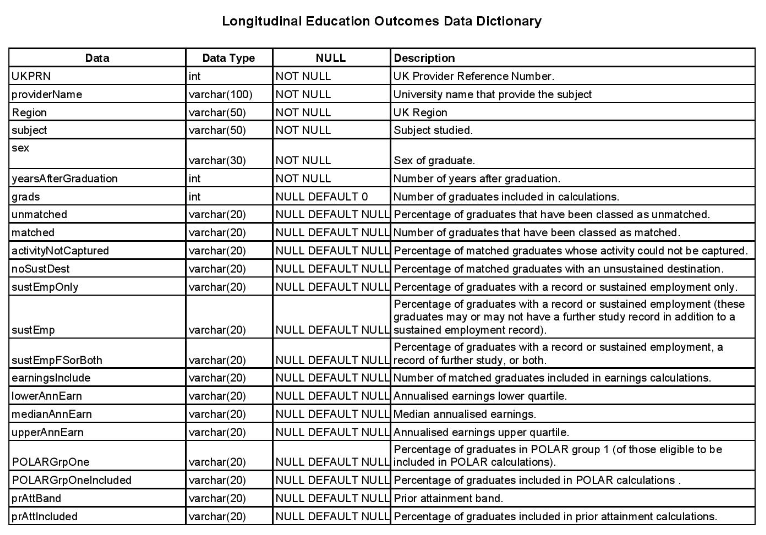
\includegraphics[width=1.0\textwidth]{Data-Dictionary/LEO.png}
	\rule{35em}{0.7pt}
	\caption[Phase 1 Longitudinal Education Outcomes (LEO) Data Dictionary]{Phase 1 Longitudinal Education Outcomes (LEO) Data Dictionary}
\end{figure}

\subsection{Phase 1 Company Data Dictionary}

\begin{figure}[H]
	\centering	
	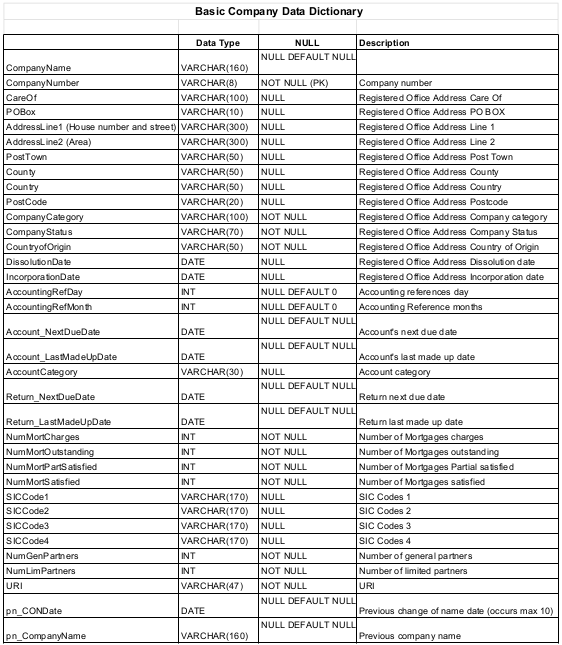
\includegraphics[width=0.9\textwidth]{Data-Dictionary/company-data-dictionary.png}
	\rule{35em}{0.5pt}
	\caption[Phase 1 Company Data Dictionary]{Phase 1 Company Data Dictionary}
\end{figure}

\subsection{Phase 1 National Statistics Postcode Lookup (NSPL) Data Dictionary}

\begin{figure}[H]
	\centering
	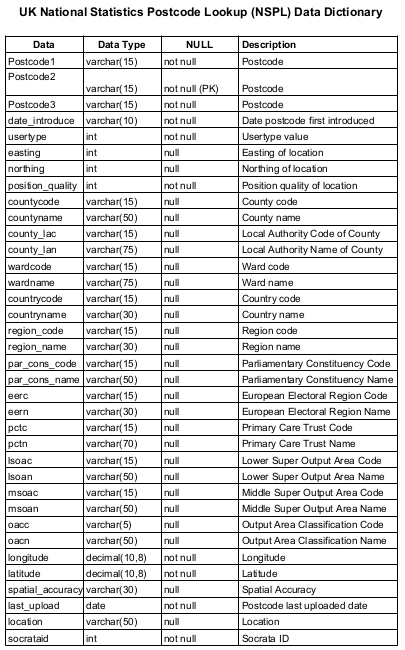
\includegraphics[width=0.8\textwidth]{Data-Dictionary/NSPL-data-dictionary.png}
	\rule{35em}{0.5pt}
	\caption[Phase 1 National Statistics Postcode Lookup (NSPL) Data Dictionary]{Phase 1 National Statistics Postcode Lookup (NSPL) Data Dictionary}
	
\end{figure}


%\setboolean{@twoside}{false}

\includepdf[pages=-, offset=75 -75]{Figures/Log/meeting-log-1-1.jpg}
\includepdf[pages=-, offset=75 -75]{Figures/Log/meeting-log-1-2.jpg}
%% \includepdf[pages=-, offset=75 -75]{Figures/Log/meeting-log-2-1.jpg}

%
\addtocontents{toc}{\vspace{2em}} 
% Add a gap in the Contents, for aesthetics

\backmatter

\end{document}